\documentclass[twoside]{book}

% Packages required by doxygen
\usepackage{fixltx2e}
\usepackage{calc}
\usepackage{doxygen}
\usepackage[export]{adjustbox} % also loads graphicx
\usepackage{graphicx}
\usepackage[utf8]{inputenc}
\usepackage{makeidx}
\usepackage{multicol}
\usepackage{multirow}
\PassOptionsToPackage{warn}{textcomp}
\usepackage{textcomp}
\usepackage[nointegrals]{wasysym}
\usepackage[table]{xcolor}

% Font selection
\usepackage[T1]{fontenc}
\usepackage[scaled=.90]{helvet}
\usepackage{courier}
\usepackage{amssymb}
\usepackage{sectsty}
\renewcommand{\familydefault}{\sfdefault}
\allsectionsfont{%
  \fontseries{bc}\selectfont%
  \color{darkgray}%
}
\renewcommand{\DoxyLabelFont}{%
  \fontseries{bc}\selectfont%
  \color{darkgray}%
}
\newcommand{\+}{\discretionary{\mbox{\scriptsize$\hookleftarrow$}}{}{}}

% Page & text layout
\usepackage{geometry}
\geometry{%
  a4paper,%
  top=2.5cm,%
  bottom=2.5cm,%
  left=2.5cm,%
  right=2.5cm%
}
\tolerance=750
\hfuzz=15pt
\hbadness=750
\setlength{\emergencystretch}{15pt}
\setlength{\parindent}{0cm}
\setlength{\parskip}{3ex plus 2ex minus 2ex}
\makeatletter
\renewcommand{\paragraph}{%
  \@startsection{paragraph}{4}{0ex}{-1.0ex}{1.0ex}{%
    \normalfont\normalsize\bfseries\SS@parafont%
  }%
}
\renewcommand{\subparagraph}{%
  \@startsection{subparagraph}{5}{0ex}{-1.0ex}{1.0ex}{%
    \normalfont\normalsize\bfseries\SS@subparafont%
  }%
}
\makeatother

% Headers & footers
\usepackage{fancyhdr}
\pagestyle{fancyplain}
\fancyhead[LE]{\fancyplain{}{\bfseries\thepage}}
\fancyhead[CE]{\fancyplain{}{}}
\fancyhead[RE]{\fancyplain{}{\bfseries\leftmark}}
\fancyhead[LO]{\fancyplain{}{\bfseries\rightmark}}
\fancyhead[CO]{\fancyplain{}{}}
\fancyhead[RO]{\fancyplain{}{\bfseries\thepage}}
\fancyfoot[LE]{\fancyplain{}{}}
\fancyfoot[CE]{\fancyplain{}{}}
\fancyfoot[RE]{\fancyplain{}{\bfseries\scriptsize Generated by Doxygen }}
\fancyfoot[LO]{\fancyplain{}{\bfseries\scriptsize Generated by Doxygen }}
\fancyfoot[CO]{\fancyplain{}{}}
\fancyfoot[RO]{\fancyplain{}{}}
\renewcommand{\footrulewidth}{0.4pt}
\renewcommand{\chaptermark}[1]{%
  \markboth{#1}{}%
}
\renewcommand{\sectionmark}[1]{%
  \markright{\thesection\ #1}%
}

% Indices & bibliography
\usepackage{natbib}
\usepackage[titles]{tocloft}
\setcounter{tocdepth}{3}
\setcounter{secnumdepth}{5}
\makeindex

% Hyperlinks (required, but should be loaded last)
\usepackage{ifpdf}
\ifpdf
  \usepackage[pdftex,pagebackref=true]{hyperref}
\else
  \usepackage[ps2pdf,pagebackref=true]{hyperref}
\fi
\hypersetup{%
  colorlinks=true,%
  linkcolor=blue,%
  citecolor=blue,%
  unicode%
}

% Custom commands
\newcommand{\clearemptydoublepage}{%
  \newpage{\pagestyle{empty}\cleardoublepage}%
}

\usepackage{caption}
\captionsetup{labelsep=space,justification=centering,font={bf},singlelinecheck=off,skip=4pt,position=top}

%===== C O N T E N T S =====

\begin{document}

% Titlepage & ToC
\hypersetup{pageanchor=false,
             bookmarksnumbered=true,
             pdfencoding=unicode
            }
\pagenumbering{alph}
\begin{titlepage}
\vspace*{7cm}
\begin{center}%
{\Large My Project }\\
\vspace*{1cm}
{\large Generated by Doxygen 1.8.13}\\
\end{center}
\end{titlepage}
\clearemptydoublepage
\pagenumbering{roman}
\tableofcontents
\clearemptydoublepage
\pagenumbering{arabic}
\hypersetup{pageanchor=true}

%--- Begin generated contents ---
\chapter{Mootii Mamo, C\+S\+CI 3081W, mamox017@umn.\+edu}
\label{index}\hypertarget{index}{}\hypertarget{index_intro_sec}{}\section{Project Transit\+Sim\+: a Proof-\/of-\/\+Concept Transit System Simulator\+: Iteration 1}\label{index_intro_sec}
Hello 
\chapter{Hierarchical Index}
\section{Class Hierarchy}
This inheritance list is sorted roughly, but not completely, alphabetically\+:\begin{DoxyCompactList}
\item \contentsline{section}{Bus}{\pageref{classBus}}{}
\item \contentsline{section}{Passenger}{\pageref{classPassenger}}{}
\item \contentsline{section}{Passenger\+Factory}{\pageref{classPassengerFactory}}{}
\item \contentsline{section}{Passenger\+Generator}{\pageref{classPassengerGenerator}}{}
\begin{DoxyCompactList}
\item \contentsline{section}{Random\+Passenger\+Generator}{\pageref{classRandomPassengerGenerator}}{}
\end{DoxyCompactList}
\item \contentsline{section}{Route}{\pageref{classRoute}}{}
\item \contentsline{section}{Simulator}{\pageref{classSimulator}}{}
\begin{DoxyCompactList}
\item \contentsline{section}{Local\+Simulator}{\pageref{classLocalSimulator}}{}
\end{DoxyCompactList}
\item \contentsline{section}{Stop}{\pageref{classStop}}{}
\end{DoxyCompactList}

\chapter{Class Index}
\section{Class List}
Here are the classes, structs, unions and interfaces with brief descriptions\+:\begin{DoxyCompactList}
\item\contentsline{section}{\hyperlink{classBus}{Bus} \\*The main class for the bus }{\pageref{classBus}}{}
\item\contentsline{section}{\hyperlink{classLocalSimulator}{Local\+Simulator} \\*The main class for a localsimulator }{\pageref{classLocalSimulator}}{}
\item\contentsline{section}{\hyperlink{classPassenger}{Passenger} \\*The main class for the passenger }{\pageref{classPassenger}}{}
\item\contentsline{section}{\hyperlink{classPassengerFactory}{Passenger\+Factory} \\*The main class for the generation of passengers }{\pageref{classPassengerFactory}}{}
\item\contentsline{section}{\hyperlink{classPassengerGenerator}{Passenger\+Generator} \\*The main class for the passenger generator }{\pageref{classPassengerGenerator}}{}
\item\contentsline{section}{\hyperlink{classRandomPassengerGenerator}{Random\+Passenger\+Generator} \\*The main class for the random passenger generator }{\pageref{classRandomPassengerGenerator}}{}
\item\contentsline{section}{\hyperlink{classRoute}{Route} \\*The main class for a route }{\pageref{classRoute}}{}
\item\contentsline{section}{\hyperlink{classSimulator}{Simulator} \\*The main class for the simulator }{\pageref{classSimulator}}{}
\item\contentsline{section}{\hyperlink{classStop}{Stop} \\*The main class for a stop }{\pageref{classStop}}{}
\end{DoxyCompactList}

\chapter{File Index}
\section{File List}
Here is a list of all documented files with brief descriptions\+:\begin{DoxyCompactList}
\item\contentsline{section}{/home/mamox017/3081\+\_\+f19/repo-\/mamox017/labs/lab08\+\_\+style\+\_\+doxy/src/\hyperlink{main_8cc}{main.\+cc} }{\pageref{main_8cc}}{}
\item\contentsline{section}{/home/mamox017/3081\+\_\+f19/repo-\/mamox017/labs/lab08\+\_\+style\+\_\+doxy/src/{\bfseries mainpage.\+h} }{\pageref{mainpage_8h}}{}
\item\contentsline{section}{/home/mamox017/3081\+\_\+f19/repo-\/mamox017/labs/lab08\+\_\+style\+\_\+doxy/src/{\bfseries passenger.\+h} }{\pageref{passenger_8h}}{}
\item\contentsline{section}{/home/mamox017/3081\+\_\+f19/repo-\/mamox017/labs/lab08\+\_\+style\+\_\+doxy/src/\hyperlink{passenger__factory_8cc}{passenger\+\_\+factory.\+cc} }{\pageref{passenger__factory_8cc}}{}
\item\contentsline{section}{/home/mamox017/3081\+\_\+f19/repo-\/mamox017/labs/lab08\+\_\+style\+\_\+doxy/src/\hyperlink{passenger__factory_8h}{passenger\+\_\+factory.\+h} }{\pageref{passenger__factory_8h}}{}
\end{DoxyCompactList}

\chapter{Class Documentation}
\hypertarget{classBus}{}\section{Bus Class Reference}
\label{classBus}\index{Bus@{Bus}}


The main class for the bus.  




{\ttfamily \#include $<$bus.\+h$>$}



Collaboration diagram for Bus\+:\nopagebreak
\begin{figure}[H]
\begin{center}
\leavevmode
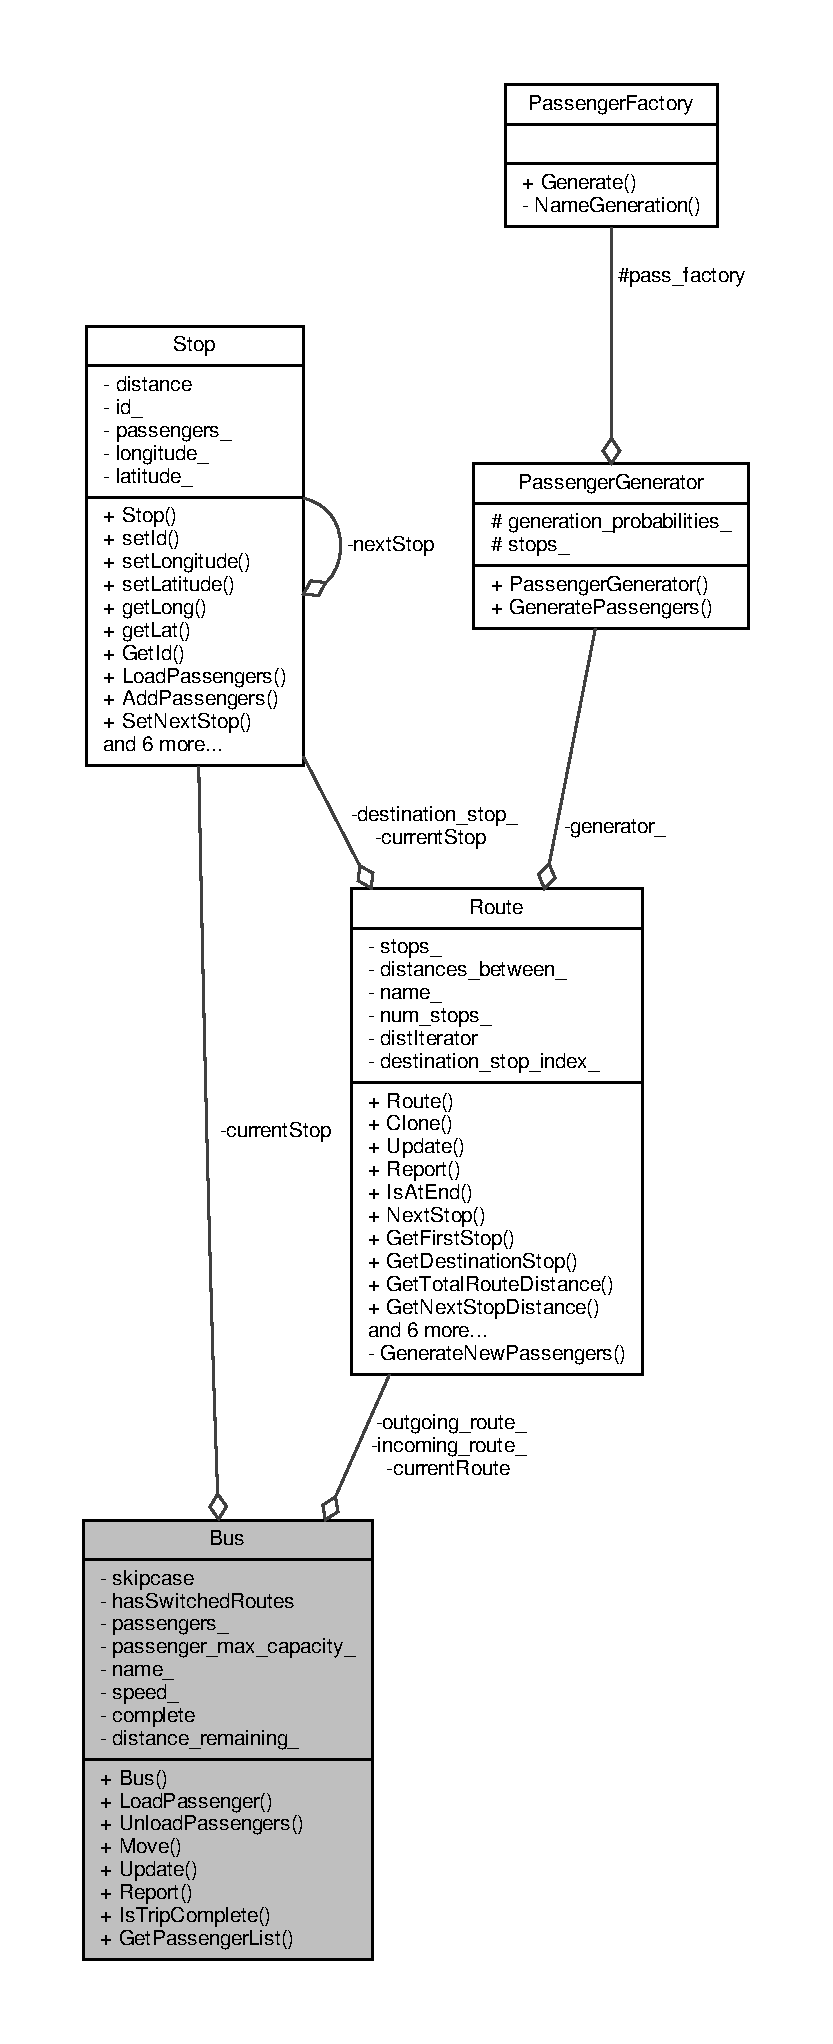
\includegraphics[height=550pt]{classBus__coll__graph}
\end{center}
\end{figure}
\subsection*{Public Member Functions}
\begin{DoxyCompactItemize}
\item 
\hyperlink{classBus_aa28c3c318b6993f3a3aebf211daa9217}{Bus} (std\+::string name, \hyperlink{classRoute}{Route} $\ast$out, \hyperlink{classRoute}{Route} $\ast$in, int capacity=60, double speed=1)
\begin{DoxyCompactList}\small\item\em The constructor function of \hyperlink{classBus}{Bus} objects. \end{DoxyCompactList}\item 
bool \hyperlink{classBus_aae72290f9daf683b3068428eee0a9ee7}{Load\+Passenger} (\hyperlink{classPassenger}{Passenger} $\ast$new\+\_\+passenger)
\begin{DoxyCompactList}\small\item\em The passenger loader function for \hyperlink{classBus}{Bus} objects. \end{DoxyCompactList}\item 
bool \hyperlink{classBus_a352bd5f926705ed4dd91d7fdea6a7fc9}{Unload\+Passengers} ()
\begin{DoxyCompactList}\small\item\em The passenger unloader function for \hyperlink{classBus}{Bus} objects. \end{DoxyCompactList}\item 
bool \hyperlink{classBus_a5e667186d6db0916ebab0e4eff3312c8}{Move} ()
\begin{DoxyCompactList}\small\item\em The motion function for \hyperlink{classBus}{Bus} objects. \end{DoxyCompactList}\item 
void \hyperlink{classBus_a9896f74f16966f7621d0dfafff0ec6b4}{Update} ()
\begin{DoxyCompactList}\small\item\em The bus updater function for \hyperlink{classBus}{Bus} objects. \end{DoxyCompactList}\item 
void \hyperlink{classBus_a695e790984f5cf7bbec85fe422466b48}{Report} (std\+::ostream \&o)
\begin{DoxyCompactList}\small\item\em The report function for \hyperlink{classBus}{Bus} objects. \end{DoxyCompactList}\item 
bool \hyperlink{classBus_a9c64b0801bf589f121fb0598b70a99b4}{Is\+Trip\+Complete} ()
\begin{DoxyCompactList}\small\item\em The trip complete checker function for \hyperlink{classBus}{Bus} objects. \end{DoxyCompactList}\item 
std\+::list$<$ \hyperlink{classPassenger}{Passenger} $\ast$ $>$ \hyperlink{classBus_a0662511d51f1c4ba7466e626be3c2ca0}{Get\+Passenger\+List} ()
\begin{DoxyCompactList}\small\item\em The bus Get\+Passenger\+List function for \hyperlink{classBus}{Bus} objects. \end{DoxyCompactList}\end{DoxyCompactItemize}
\subsection*{Private Attributes}
\begin{DoxyCompactItemize}
\item 
\mbox{\Hypertarget{classBus_a71d4efb1f0e2810c712d2b04eaa9f909}\label{classBus_a71d4efb1f0e2810c712d2b04eaa9f909}} 
\hyperlink{classStop}{Stop} $\ast$ {\bfseries current\+Stop}
\item 
\mbox{\Hypertarget{classBus_aca3e8ae5c42858f0f9e59c53270ee04e}\label{classBus_aca3e8ae5c42858f0f9e59c53270ee04e}} 
bool {\bfseries skipcase}
\item 
\mbox{\Hypertarget{classBus_a1e9e0ddf70d42b3320669f275a586587}\label{classBus_a1e9e0ddf70d42b3320669f275a586587}} 
bool {\bfseries has\+Switched\+Routes}
\item 
\mbox{\Hypertarget{classBus_a009d8dacb64ef5dc6fa9a8f3511face9}\label{classBus_a009d8dacb64ef5dc6fa9a8f3511face9}} 
bool {\bfseries first\+Iter}
\item 
\mbox{\Hypertarget{classBus_a4a6e51d12fa70cbf9e973e82090773f3}\label{classBus_a4a6e51d12fa70cbf9e973e82090773f3}} 
std\+::list$<$ \hyperlink{classPassenger}{Passenger} $\ast$ $>$ {\bfseries passengers\+\_\+}
\item 
\mbox{\Hypertarget{classBus_a0f8a0586923d96c085a6d33b74150962}\label{classBus_a0f8a0586923d96c085a6d33b74150962}} 
int {\bfseries passenger\+\_\+max\+\_\+capacity\+\_\+}
\item 
\mbox{\Hypertarget{classBus_a414fa2321dd325141c60741eb838972d}\label{classBus_a414fa2321dd325141c60741eb838972d}} 
std\+::string {\bfseries name\+\_\+}
\item 
\mbox{\Hypertarget{classBus_acae5a7639b0c5b3c4a1d1f888ac18ce1}\label{classBus_acae5a7639b0c5b3c4a1d1f888ac18ce1}} 
double {\bfseries speed\+\_\+}
\item 
\mbox{\Hypertarget{classBus_a625684b3e464f90f822f6303d6113b49}\label{classBus_a625684b3e464f90f822f6303d6113b49}} 
\hyperlink{classRoute}{Route} $\ast$ {\bfseries outgoing\+\_\+route\+\_\+}
\item 
\mbox{\Hypertarget{classBus_a393eb8015c87cc306a4ce18bf3f19956}\label{classBus_a393eb8015c87cc306a4ce18bf3f19956}} 
\hyperlink{classRoute}{Route} $\ast$ {\bfseries incoming\+\_\+route\+\_\+}
\item 
\mbox{\Hypertarget{classBus_a0a220de5b56257d6835ae58a95f2c352}\label{classBus_a0a220de5b56257d6835ae58a95f2c352}} 
\hyperlink{classRoute}{Route} $\ast$ {\bfseries current\+Route}
\item 
\mbox{\Hypertarget{classBus_ae8b6cf1028a4f5dffd82c1423f17e58e}\label{classBus_ae8b6cf1028a4f5dffd82c1423f17e58e}} 
bool {\bfseries complete}
\item 
\mbox{\Hypertarget{classBus_ae0e153e41426834bb6c15ffa90bca417}\label{classBus_ae0e153e41426834bb6c15ffa90bca417}} 
double {\bfseries distance\+\_\+remaining\+\_\+}
\end{DoxyCompactItemize}


\subsection{Detailed Description}
The main class for the bus. 

Creates a new instance of a \hyperlink{classBus}{Bus} object. 

\subsection{Constructor \& Destructor Documentation}
\mbox{\Hypertarget{classBus_aa28c3c318b6993f3a3aebf211daa9217}\label{classBus_aa28c3c318b6993f3a3aebf211daa9217}} 
\index{Bus@{Bus}!Bus@{Bus}}
\index{Bus@{Bus}!Bus@{Bus}}
\subsubsection{\texorpdfstring{Bus()}{Bus()}}
{\footnotesize\ttfamily Bus\+::\+Bus (\begin{DoxyParamCaption}\item[{std\+::string}]{name,  }\item[{\hyperlink{classRoute}{Route} $\ast$}]{out,  }\item[{\hyperlink{classRoute}{Route} $\ast$}]{in,  }\item[{int}]{capacity = {\ttfamily 60},  }\item[{double}]{speed = {\ttfamily 1} }\end{DoxyParamCaption})}



The constructor function of \hyperlink{classBus}{Bus} objects. 

This creates a bus object with given attributes as arguments.


\begin{DoxyParams}[1]{Parameters}
\mbox{\tt in}  & {\em std\+::string} & name Current stop, name attribute of the \hyperlink{classBus}{Bus} object \\
\hline
\mbox{\tt in}  & {\em \hyperlink{classRoute}{Route}} & $\ast$ out, outgoing route of the bus, used after in \\
\hline
\mbox{\tt in}  & {\em \hyperlink{classRoute}{Route}} & $\ast$ in, incoming route of the bus, traversed first \\
\hline
\mbox{\tt in}  & {\em int} & capacity, maximum number of passengers in passenger\+\_\+ list \\
\hline
\mbox{\tt in}  & {\em double} & speed, number at which distance\+\_\+remaining\+\_\+ decreases\\
\hline
\end{DoxyParams}
\begin{DoxyReturn}{Returns}
\hyperlink{classBus}{Bus} object with name, outgoing route, incoming route, cap, and speed 
\end{DoxyReturn}


\subsection{Member Function Documentation}
\mbox{\Hypertarget{classBus_a0662511d51f1c4ba7466e626be3c2ca0}\label{classBus_a0662511d51f1c4ba7466e626be3c2ca0}} 
\index{Bus@{Bus}!Get\+Passenger\+List@{Get\+Passenger\+List}}
\index{Get\+Passenger\+List@{Get\+Passenger\+List}!Bus@{Bus}}
\subsubsection{\texorpdfstring{Get\+Passenger\+List()}{GetPassengerList()}}
{\footnotesize\ttfamily std\+::list$<$ \hyperlink{classPassenger}{Passenger} $\ast$ $>$ Bus\+::\+Get\+Passenger\+List (\begin{DoxyParamCaption}{ }\end{DoxyParamCaption})}



The bus Get\+Passenger\+List function for \hyperlink{classBus}{Bus} objects. 

This function accesses the private member variable passenger\+\_\+

\begin{DoxyReturn}{Returns}
std\+::list$<$\+Passenger $\ast$$>$ list of passengers onboard bus 
\end{DoxyReturn}
\mbox{\Hypertarget{classBus_a9c64b0801bf589f121fb0598b70a99b4}\label{classBus_a9c64b0801bf589f121fb0598b70a99b4}} 
\index{Bus@{Bus}!Is\+Trip\+Complete@{Is\+Trip\+Complete}}
\index{Is\+Trip\+Complete@{Is\+Trip\+Complete}!Bus@{Bus}}
\subsubsection{\texorpdfstring{Is\+Trip\+Complete()}{IsTripComplete()}}
{\footnotesize\ttfamily bool Bus\+::\+Is\+Trip\+Complete (\begin{DoxyParamCaption}{ }\end{DoxyParamCaption})}



The trip complete checker function for \hyperlink{classBus}{Bus} objects. 

This function checks if the bus is at the end of both the incoming and outgoing routes by using Is\+At\+End() {\itshape \mbox{[}E\+D\+IT\mbox{]}} This accessor function retrieves the member variable complete

\begin{DoxyReturn}{Returns}
bool object that is true if complete or false if incomplete 
\end{DoxyReturn}
\mbox{\Hypertarget{classBus_aae72290f9daf683b3068428eee0a9ee7}\label{classBus_aae72290f9daf683b3068428eee0a9ee7}} 
\index{Bus@{Bus}!Load\+Passenger@{Load\+Passenger}}
\index{Load\+Passenger@{Load\+Passenger}!Bus@{Bus}}
\subsubsection{\texorpdfstring{Load\+Passenger()}{LoadPassenger()}}
{\footnotesize\ttfamily bool Bus\+::\+Load\+Passenger (\begin{DoxyParamCaption}\item[{\hyperlink{classPassenger}{Passenger} $\ast$}]{new\+\_\+passenger }\end{DoxyParamCaption})}



The passenger loader function for \hyperlink{classBus}{Bus} objects. 

This function loads a passenger onto the bus if the capacity isn\textquotesingle{}t reached.


\begin{DoxyParams}[1]{Parameters}
\mbox{\tt in}  & {\em \hyperlink{classPassenger}{Passenger}} & $\ast$ new\+\_\+passenger, pointer to passenger to be loaded\\
\hline
\end{DoxyParams}
\begin{DoxyReturn}{Returns}
Boolean object determining whether or not the load was successful 
\end{DoxyReturn}
\mbox{\Hypertarget{classBus_a5e667186d6db0916ebab0e4eff3312c8}\label{classBus_a5e667186d6db0916ebab0e4eff3312c8}} 
\index{Bus@{Bus}!Move@{Move}}
\index{Move@{Move}!Bus@{Bus}}
\subsubsection{\texorpdfstring{Move()}{Move()}}
{\footnotesize\ttfamily bool Bus\+::\+Move (\begin{DoxyParamCaption}{ }\end{DoxyParamCaption})}



The motion function for \hyperlink{classBus}{Bus} objects. 

This function moves the bus by decreasing the distance\+\_\+remaining\+\_\+ by speed. If the distance\+\_\+remaining\+\_\+ is less than or equal to 0, progresses to next stop.

\begin{DoxyReturn}{Returns}
bool object determining whether or not at a stop 
\end{DoxyReturn}
\mbox{\Hypertarget{classBus_a695e790984f5cf7bbec85fe422466b48}\label{classBus_a695e790984f5cf7bbec85fe422466b48}} 
\index{Bus@{Bus}!Report@{Report}}
\index{Report@{Report}!Bus@{Bus}}
\subsubsection{\texorpdfstring{Report()}{Report()}}
{\footnotesize\ttfamily void Bus\+::\+Report (\begin{DoxyParamCaption}\item[{std\+::ostream \&}]{o }\end{DoxyParamCaption})}



The report function for \hyperlink{classBus}{Bus} objects. 

This function reports the bus\textquotesingle{}s attributes to a given output stream.


\begin{DoxyParams}[1]{Parameters}
\mbox{\tt in}  & {\em std\+::ostream\&} & o, the output stream to which the information is sent.\\
\hline
\end{DoxyParams}
\begin{DoxyReturn}{Returns}
void 
\end{DoxyReturn}
\mbox{\Hypertarget{classBus_a352bd5f926705ed4dd91d7fdea6a7fc9}\label{classBus_a352bd5f926705ed4dd91d7fdea6a7fc9}} 
\index{Bus@{Bus}!Unload\+Passengers@{Unload\+Passengers}}
\index{Unload\+Passengers@{Unload\+Passengers}!Bus@{Bus}}
\subsubsection{\texorpdfstring{Unload\+Passengers()}{UnloadPassengers()}}
{\footnotesize\ttfamily bool Bus\+::\+Unload\+Passengers (\begin{DoxyParamCaption}{ }\end{DoxyParamCaption})}



The passenger unloader function for \hyperlink{classBus}{Bus} objects. 

This function unloads a passenger off the bus.

\begin{DoxyReturn}{Returns}
bool object determining whether or not the unload was successful 
\end{DoxyReturn}
\mbox{\Hypertarget{classBus_a9896f74f16966f7621d0dfafff0ec6b4}\label{classBus_a9896f74f16966f7621d0dfafff0ec6b4}} 
\index{Bus@{Bus}!Update@{Update}}
\index{Update@{Update}!Bus@{Bus}}
\subsubsection{\texorpdfstring{Update()}{Update()}}
{\footnotesize\ttfamily void Bus\+::\+Update (\begin{DoxyParamCaption}{ }\end{DoxyParamCaption})}



The bus updater function for \hyperlink{classBus}{Bus} objects. 

This function updates the bus\textquotesingle{}s state if the trip is not complete. If the bus is at a stop, as determined by \hyperlink{classBus_a5e667186d6db0916ebab0e4eff3312c8}{Move()}, passengers will be unloaded and loaded.

\begin{DoxyReturn}{Returns}
void 
\end{DoxyReturn}


The documentation for this class was generated from the following files\+:\begin{DoxyCompactItemize}
\item 
/home/mamox017/3081\+\_\+f19/repo-\/mamox017/project/src/\hyperlink{bus_8h}{bus.\+h}\item 
/home/mamox017/3081\+\_\+f19/repo-\/mamox017/project/src/bus.\+cc\end{DoxyCompactItemize}

\hypertarget{classLocalSimulator}{}\section{Local\+Simulator Class Reference}
\label{classLocalSimulator}\index{Local\+Simulator@{Local\+Simulator}}


The main class for a localsimulator.  




{\ttfamily \#include $<$local\+\_\+simulator.\+h$>$}



Inheritance diagram for Local\+Simulator\+:\nopagebreak
\begin{figure}[H]
\begin{center}
\leavevmode
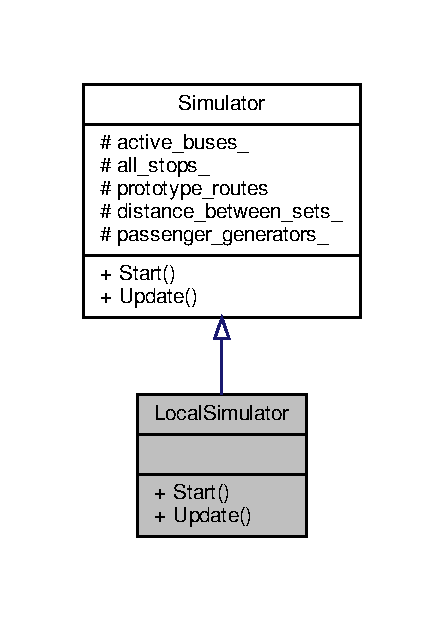
\includegraphics[width=215pt]{classLocalSimulator__inherit__graph}
\end{center}
\end{figure}


Collaboration diagram for Local\+Simulator\+:\nopagebreak
\begin{figure}[H]
\begin{center}
\leavevmode
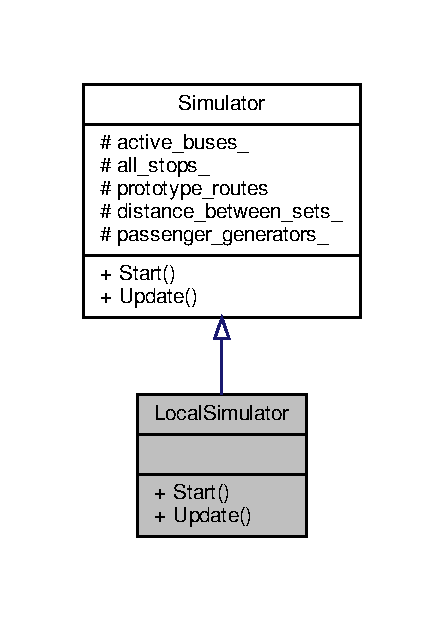
\includegraphics[width=215pt]{classLocalSimulator__coll__graph}
\end{center}
\end{figure}
\subsection*{Public Member Functions}
\begin{DoxyCompactItemize}
\item 
bool \hyperlink{classLocalSimulator_a380634942668855dd1da8276b270b362}{Start} () override
\begin{DoxyCompactList}\small\item\em The Start function for localsimulator objects. \end{DoxyCompactList}\item 
bool \hyperlink{classLocalSimulator_ac98ba1a401ad204dd5169934adb02684}{Update} () override
\begin{DoxyCompactList}\small\item\em The Update function for localsimulator objects. \end{DoxyCompactList}\end{DoxyCompactItemize}
\subsection*{Private Attributes}
\begin{DoxyCompactItemize}
\item 
\mbox{\Hypertarget{classLocalSimulator_a1c92b8c58df2b015753bd451bc469299}\label{classLocalSimulator_a1c92b8c58df2b015753bd451bc469299}} 
std\+::vector$<$ int $>$ {\bfseries bus\+\_\+counters\+\_\+}
\item 
\mbox{\Hypertarget{classLocalSimulator_afe5ff08ca4c982f774b6f924e2844689}\label{classLocalSimulator_afe5ff08ca4c982f774b6f924e2844689}} 
std\+::vector$<$ int $>$ {\bfseries bus\+\_\+start\+\_\+timings\+\_\+}
\item 
\mbox{\Hypertarget{classLocalSimulator_a161826601c14be88063cb8b2d1bee552}\label{classLocalSimulator_a161826601c14be88063cb8b2d1bee552}} 
std\+::vector$<$ int $>$ {\bfseries time\+\_\+since\+\_\+last\+\_\+bus\+\_\+generation\+\_\+}
\item 
\mbox{\Hypertarget{classLocalSimulator_a1acd308212f56e1d37eca95a2bc5d2f4}\label{classLocalSimulator_a1acd308212f56e1d37eca95a2bc5d2f4}} 
int {\bfseries simulation\+\_\+time\+\_\+elapsed\+\_\+}
\end{DoxyCompactItemize}
\subsection*{Additional Inherited Members}


\subsection{Detailed Description}
The main class for a localsimulator. 

Creates a new instance of a localsimulator object. 

\subsection{Member Function Documentation}
\mbox{\Hypertarget{classLocalSimulator_a380634942668855dd1da8276b270b362}\label{classLocalSimulator_a380634942668855dd1da8276b270b362}} 
\index{Local\+Simulator@{Local\+Simulator}!Start@{Start}}
\index{Start@{Start}!Local\+Simulator@{Local\+Simulator}}
\subsubsection{\texorpdfstring{Start()}{Start()}}
{\footnotesize\ttfamily bool Local\+Simulator\+::\+Start (\begin{DoxyParamCaption}{ }\end{DoxyParamCaption})\hspace{0.3cm}{\ttfamily [override]}, {\ttfamily [virtual]}}



The Start function for localsimulator objects. 

This function overrides the base class function to start a simulation of given situations.

\begin{DoxyReturn}{Returns}
bool = 0, indicates whether simulation successfully starts 
\end{DoxyReturn}


Implements \hyperlink{classSimulator_a0db68bef442ba6061a5f38189bbe3512}{Simulator}.

\mbox{\Hypertarget{classLocalSimulator_ac98ba1a401ad204dd5169934adb02684}\label{classLocalSimulator_ac98ba1a401ad204dd5169934adb02684}} 
\index{Local\+Simulator@{Local\+Simulator}!Update@{Update}}
\index{Update@{Update}!Local\+Simulator@{Local\+Simulator}}
\subsubsection{\texorpdfstring{Update()}{Update()}}
{\footnotesize\ttfamily bool Local\+Simulator\+::\+Update (\begin{DoxyParamCaption}{ }\end{DoxyParamCaption})\hspace{0.3cm}{\ttfamily [override]}, {\ttfamily [virtual]}}



The Update function for localsimulator objects. 

This function overrides the base class function to update a simulation of given situations.

\begin{DoxyReturn}{Returns}
bool = 0, indicates whether simulation successfully updates 
\end{DoxyReturn}


Implements \hyperlink{classSimulator_a7a5a1cbfa1e0cf9b82fe9d2e4b3b80ae}{Simulator}.



The documentation for this class was generated from the following files\+:\begin{DoxyCompactItemize}
\item 
/home/mamox017/3081\+\_\+f19/repo-\/mamox017/project/src/\hyperlink{local__simulator_8h}{local\+\_\+simulator.\+h}\item 
/home/mamox017/3081\+\_\+f19/repo-\/mamox017/project/src/\hyperlink{local__simulator_8cc}{local\+\_\+simulator.\+cc}\end{DoxyCompactItemize}

\hypertarget{classPassenger}{}\section{Passenger Class Reference}
\label{classPassenger}\index{Passenger@{Passenger}}


The main class for a passenger.  




{\ttfamily \#include $<$passenger.\+h$>$}



Collaboration diagram for Passenger\+:\nopagebreak
\begin{figure}[H]
\begin{center}
\leavevmode
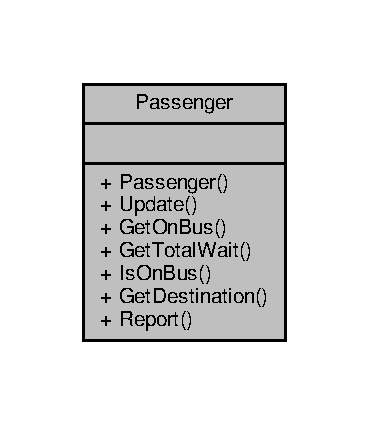
\includegraphics[width=177pt]{classPassenger__coll__graph}
\end{center}
\end{figure}
\subsection*{Public Member Functions}
\begin{DoxyCompactItemize}
\item 
\hyperlink{classPassenger_a5c3addb9a6fd03e5e5642ed844e2702c}{Passenger} (int=-\/1, std\+::string=\char`\"{}Nobody\char`\"{})
\begin{DoxyCompactList}\small\item\em constructor of a \hyperlink{classPassenger}{Passenger} \end{DoxyCompactList}\item 
\mbox{\Hypertarget{classPassenger_a960de3b29fc17a2c2d79c0b79d5cf299}\label{classPassenger_a960de3b29fc17a2c2d79c0b79d5cf299}} 
void {\bfseries Update} ()
\item 
\mbox{\Hypertarget{classPassenger_ae2ba639cfef39781ac079778578bd9fe}\label{classPassenger_ae2ba639cfef39781ac079778578bd9fe}} 
void {\bfseries Get\+On\+Bus} ()
\item 
\mbox{\Hypertarget{classPassenger_a25158560f790ef7ef06d94c414b34f25}\label{classPassenger_a25158560f790ef7ef06d94c414b34f25}} 
int {\bfseries Get\+Total\+Wait} () const
\item 
\mbox{\Hypertarget{classPassenger_a2acf008ec444afcc859b914ee24add0e}\label{classPassenger_a2acf008ec444afcc859b914ee24add0e}} 
bool {\bfseries Is\+On\+Bus} () const
\item 
\mbox{\Hypertarget{classPassenger_a49db0ee527377aae6077df190a11501c}\label{classPassenger_a49db0ee527377aae6077df190a11501c}} 
int {\bfseries Get\+Destination} () const
\item 
\mbox{\Hypertarget{classPassenger_ac54ce797e412a4895febe10f07dc5df5}\label{classPassenger_ac54ce797e412a4895febe10f07dc5df5}} 
void {\bfseries Report} () const
\end{DoxyCompactItemize}


\subsection{Detailed Description}
The main class for a passenger. 

Creates a passenger, if there is none, it defaults to 1 or gives name Nobody has getters for destination and information 

\subsection{Constructor \& Destructor Documentation}
\mbox{\Hypertarget{classPassenger_a5c3addb9a6fd03e5e5642ed844e2702c}\label{classPassenger_a5c3addb9a6fd03e5e5642ed844e2702c}} 
\index{Passenger@{Passenger}!Passenger@{Passenger}}
\index{Passenger@{Passenger}!Passenger@{Passenger}}
\subsubsection{\texorpdfstring{Passenger()}{Passenger()}}
{\footnotesize\ttfamily Passenger\+::\+Passenger (\begin{DoxyParamCaption}\item[{int}]{destination\+\_\+stop\+\_\+id = {\ttfamily -\/1},  }\item[{std\+::string}]{name = {\ttfamily \char`\"{}Nobody\char`\"{}} }\end{DoxyParamCaption})\hspace{0.3cm}{\ttfamily [explicit]}}



constructor of a \hyperlink{classPassenger}{Passenger} 


\begin{DoxyParams}[1]{Parameters}
\mbox{\tt in}  & {\em passenger\textquotesingle{}s} & destination id \\
\hline
\mbox{\tt in}  & {\em passenger\textquotesingle{}s} & name\\
\hline
\end{DoxyParams}
\begin{DoxyReturn}{Returns}
\hyperlink{classPassenger}{Passenger} object 
\end{DoxyReturn}


The documentation for this class was generated from the following files\+:\begin{DoxyCompactItemize}
\item 
/home/mamox017/3081\+\_\+f19/repo-\/mamox017/labs/lab08\+\_\+style\+\_\+doxy/src/passenger.\+h\item 
/home/mamox017/3081\+\_\+f19/repo-\/mamox017/labs/lab08\+\_\+style\+\_\+doxy/src/passenger.\+cc\end{DoxyCompactItemize}

\hypertarget{classPassengerFactory}{}\section{Passenger\+Factory Class Reference}
\label{classPassengerFactory}\index{Passenger\+Factory@{Passenger\+Factory}}


The main class for the generation of passengers.  




{\ttfamily \#include $<$passenger\+\_\+factory.\+h$>$}



Collaboration diagram for Passenger\+Factory\+:\nopagebreak
\begin{figure}[H]
\begin{center}
\leavevmode
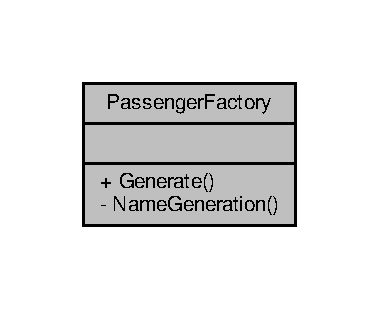
\includegraphics[width=176pt]{classPassengerFactory__coll__graph}
\end{center}
\end{figure}
\subsection*{Static Public Member Functions}
\begin{DoxyCompactItemize}
\item 
static \hyperlink{classPassenger}{Passenger} $\ast$ \hyperlink{classPassengerFactory_a2952ba78ceb285f445bc768d287230d2}{Generate} (int, int)
\begin{DoxyCompactList}\small\item\em Generation of a passenger with a randomized name and random destination within bounds. \end{DoxyCompactList}\end{DoxyCompactItemize}


\subsection{Detailed Description}
The main class for the generation of passengers. 

Calls to \hyperlink{classPassengerFactory_a2952ba78ceb285f445bc768d287230d2}{Generate} function to get a new instance of a passenger. This is a static call, not requiring an instance to invoke the method. 

\subsection{Member Function Documentation}
\mbox{\Hypertarget{classPassengerFactory_a2952ba78ceb285f445bc768d287230d2}\label{classPassengerFactory_a2952ba78ceb285f445bc768d287230d2}} 
\index{Passenger\+Factory@{Passenger\+Factory}!Generate@{Generate}}
\index{Generate@{Generate}!Passenger\+Factory@{Passenger\+Factory}}
\subsubsection{\texorpdfstring{Generate()}{Generate()}}
{\footnotesize\ttfamily \hyperlink{classPassenger}{Passenger} $\ast$ Passenger\+Factory\+::\+Generate (\begin{DoxyParamCaption}\item[{int}]{curr\+\_\+stop,  }\item[{int}]{last\+\_\+stop }\end{DoxyParamCaption})\hspace{0.3cm}{\ttfamily [static]}}



Generation of a passenger with a randomized name and random destination within bounds. 

This function will be used for simulation purposes.


\begin{DoxyParams}[1]{Parameters}
\mbox{\tt in}  & {\em curr\+\_\+stop} & Current stop, left bound (not-\/inclusive) \\
\hline
\mbox{\tt in}  & {\em last\+\_\+stop} & Last stop, right bound (inclusive)\\
\hline
\end{DoxyParams}
\begin{DoxyReturn}{Returns}
\hyperlink{classPassenger}{Passenger} object with name and destination. 
\end{DoxyReturn}


The documentation for this class was generated from the following files\+:\begin{DoxyCompactItemize}
\item 
/home/mamox017/3081\+\_\+f19/repo-\/mamox017/labs/lab08\+\_\+style\+\_\+doxy/src/\hyperlink{passenger__factory_8h}{passenger\+\_\+factory.\+h}\item 
/home/mamox017/3081\+\_\+f19/repo-\/mamox017/labs/lab08\+\_\+style\+\_\+doxy/src/\hyperlink{passenger__factory_8cc}{passenger\+\_\+factory.\+cc}\end{DoxyCompactItemize}

\hypertarget{classPassengerGenerator}{}\section{Passenger\+Generator Class Reference}
\label{classPassengerGenerator}\index{Passenger\+Generator@{Passenger\+Generator}}


<<<<<<< HEAD
The main class for the passenger generator.  




{\ttfamily \#include $<$passenger\+\_\+generator.\+h$>$}



Inheritance diagram for Passenger\+Generator\+:\nopagebreak
=======
Inheritance diagram for Passenger\+Generator\+:
\nopagebreak
>>>>>>> master
\begin{figure}[H]
\begin{center}
\leavevmode
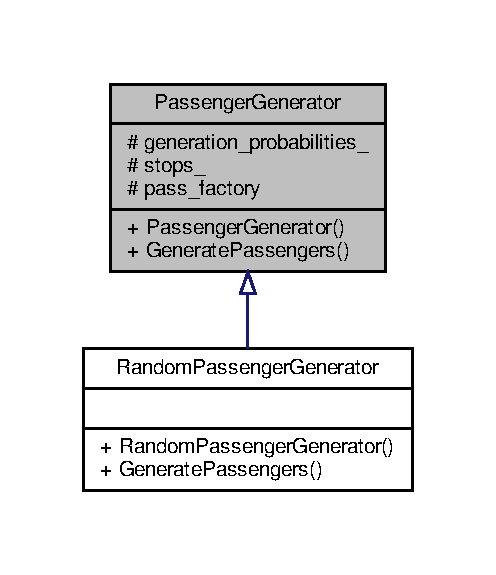
\includegraphics[width=238pt]{classPassengerGenerator__inherit__graph}
\end{center}
\end{figure}


<<<<<<< HEAD
Collaboration diagram for Passenger\+Generator\+:\nopagebreak
=======
Collaboration diagram for Passenger\+Generator\+:
\nopagebreak
>>>>>>> master
\begin{figure}[H]
\begin{center}
\leavevmode
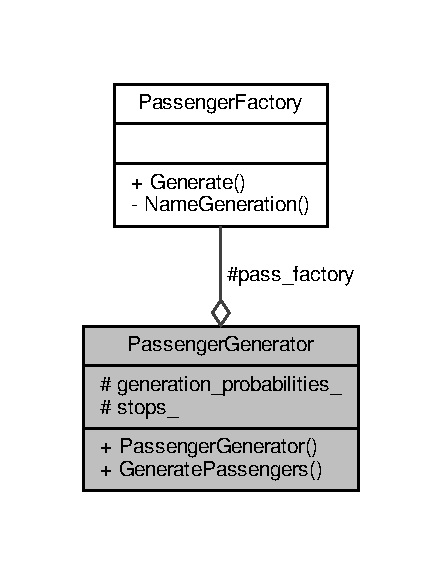
\includegraphics[width=212pt]{classPassengerGenerator__coll__graph}
\end{center}
\end{figure}
\subsection*{Public Member Functions}
\begin{DoxyCompactItemize}
\item 
<<<<<<< HEAD
\hyperlink{classPassengerGenerator_a33eeed8b68d5d596ceef5381c697e49d}{Passenger\+Generator} (std\+::list$<$ double $>$, std\+::list$<$ \hyperlink{classStop}{Stop} $\ast$$>$)
\begin{DoxyCompactList}\small\item\em Constructs a passenger generator with a double list and \hyperlink{classStop}{Stop} $\ast$ list. \end{DoxyCompactList}\item 
virtual int \hyperlink{classPassengerGenerator_ad2db96a13b34fcf35977287c06b31d47}{Generate\+Passengers} ()=0
\begin{DoxyCompactList}\small\item\em The generate passengers function for \hyperlink{classPassengerGenerator}{Passenger\+Generator} objects. \end{DoxyCompactList}\end{DoxyCompactItemize}
=======
\mbox{\Hypertarget{classPassengerGenerator_a33eeed8b68d5d596ceef5381c697e49d}\label{classPassengerGenerator_a33eeed8b68d5d596ceef5381c697e49d}} 
{\bfseries Passenger\+Generator} (std\+::list$<$ double $>$, std\+::list$<$ \hyperlink{classStop}{Stop} $\ast$$>$)
\item 
\mbox{\Hypertarget{classPassengerGenerator_ad2db96a13b34fcf35977287c06b31d47}\label{classPassengerGenerator_ad2db96a13b34fcf35977287c06b31d47}} 
virtual int {\bfseries Generate\+Passengers} ()=0
\end{DoxyCompactItemize}
>>>>>>> master
\subsection*{Protected Attributes}
\begin{DoxyCompactItemize}
\item 
\mbox{\Hypertarget{classPassengerGenerator_a855471e5532fec3f387a6340f928d43a}\label{classPassengerGenerator_a855471e5532fec3f387a6340f928d43a}} 
std\+::list$<$ double $>$ {\bfseries generation\+\_\+probabilities\+\_\+}
\item 
\mbox{\Hypertarget{classPassengerGenerator_ab09ab7ca9104385ae007d05a6e957884}\label{classPassengerGenerator_ab09ab7ca9104385ae007d05a6e957884}} 
std\+::list$<$ \hyperlink{classStop}{Stop} $\ast$ $>$ {\bfseries stops\+\_\+}
\item 
\mbox{\Hypertarget{classPassengerGenerator_a3fb4e7939da69cd257680761488f39ac}\label{classPassengerGenerator_a3fb4e7939da69cd257680761488f39ac}} 
\hyperlink{classPassengerFactory}{Passenger\+Factory} $\ast$ {\bfseries pass\+\_\+factory}
\end{DoxyCompactItemize}


<<<<<<< HEAD
\subsection{Detailed Description}
The main class for the passenger generator. 

Creates a new instance of a \hyperlink{classPassengerGenerator}{Passenger\+Generator} object. 

\subsection{Constructor \& Destructor Documentation}
\mbox{\Hypertarget{classPassengerGenerator_a33eeed8b68d5d596ceef5381c697e49d}\label{classPassengerGenerator_a33eeed8b68d5d596ceef5381c697e49d}} 
\index{Passenger\+Generator@{Passenger\+Generator}!Passenger\+Generator@{Passenger\+Generator}}
\index{Passenger\+Generator@{Passenger\+Generator}!Passenger\+Generator@{Passenger\+Generator}}
\subsubsection{\texorpdfstring{Passenger\+Generator()}{PassengerGenerator()}}
{\footnotesize\ttfamily Passenger\+Generator\+::\+Passenger\+Generator (\begin{DoxyParamCaption}\item[{std\+::list$<$ double $>$}]{probs,  }\item[{std\+::list$<$ \hyperlink{classStop}{Stop} $\ast$$>$}]{stops }\end{DoxyParamCaption})}



Constructs a passenger generator with a double list and \hyperlink{classStop}{Stop} $\ast$ list. 


\begin{DoxyParams}[1]{Parameters}
\mbox{\tt in}  & {\em std\+::list$<$double$>$} & holding the probabilities of generation \\
\hline
\mbox{\tt in}  & {\em std\+::list$<$\+Stop} & $\ast$$>$ holding the stops to generate passengers on\\
\hline
\end{DoxyParams}
\begin{DoxyReturn}{Returns}
\hyperlink{classPassengerGenerator}{Passenger\+Generator} object with double and \hyperlink{classStop}{Stop} $\ast$ list 
\end{DoxyReturn}


\subsection{Member Function Documentation}
\mbox{\Hypertarget{classPassengerGenerator_ad2db96a13b34fcf35977287c06b31d47}\label{classPassengerGenerator_ad2db96a13b34fcf35977287c06b31d47}} 
\index{Passenger\+Generator@{Passenger\+Generator}!Generate\+Passengers@{Generate\+Passengers}}
\index{Generate\+Passengers@{Generate\+Passengers}!Passenger\+Generator@{Passenger\+Generator}}
\subsubsection{\texorpdfstring{Generate\+Passengers()}{GeneratePassengers()}}
{\footnotesize\ttfamily virtual int Passenger\+Generator\+::\+Generate\+Passengers (\begin{DoxyParamCaption}{ }\end{DoxyParamCaption})\hspace{0.3cm}{\ttfamily [pure virtual]}}



The generate passengers function for \hyperlink{classPassengerGenerator}{Passenger\+Generator} objects. 

This pure virtual function is to be used by inheriting classes to generate passengers on the \hyperlink{classStop}{Stop} $\ast$ list with the probabilities from the double list.

\begin{DoxyReturn}{Returns}
int = 0, number of passengers generated 
\end{DoxyReturn}


Implemented in \hyperlink{classRandomPassengerGenerator_aba2d80cde33371cf9c3d033f1b8ba6b8}{Random\+Passenger\+Generator}.



=======
>>>>>>> master
The documentation for this class was generated from the following files\+:\begin{DoxyCompactItemize}
\item 
/home/mamox017/3081\+\_\+f19/repo-\/mamox017/project/src/\hyperlink{passenger__generator_8h}{passenger\+\_\+generator.\+h}\item 
/home/mamox017/3081\+\_\+f19/repo-\/mamox017/project/src/\hyperlink{passenger__generator_8cc}{passenger\+\_\+generator.\+cc}\end{DoxyCompactItemize}

\hypertarget{classRandomPassengerGenerator}{}\section{Random\+Passenger\+Generator Class Reference}
\label{classRandomPassengerGenerator}\index{Random\+Passenger\+Generator@{Random\+Passenger\+Generator}}


The main class for the random passenger generator.  




{\ttfamily \#include $<$random\+\_\+passenger\+\_\+generator.\+h$>$}



Inheritance diagram for Random\+Passenger\+Generator\+:\nopagebreak
\begin{figure}[H]
\begin{center}
\leavevmode
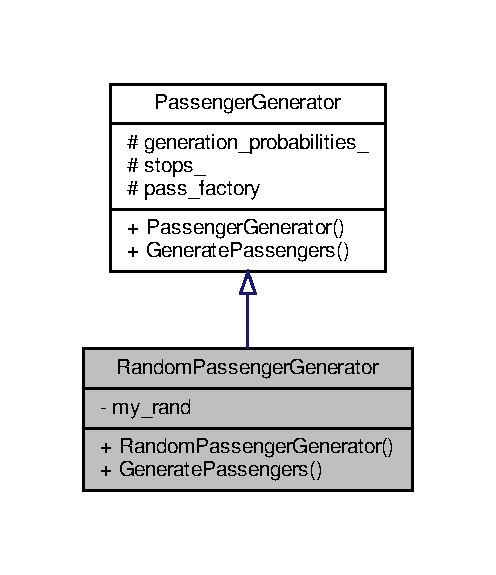
\includegraphics[width=238pt]{classRandomPassengerGenerator__inherit__graph}
\end{center}
\end{figure}


Collaboration diagram for Random\+Passenger\+Generator\+:\nopagebreak
\begin{figure}[H]
\begin{center}
\leavevmode
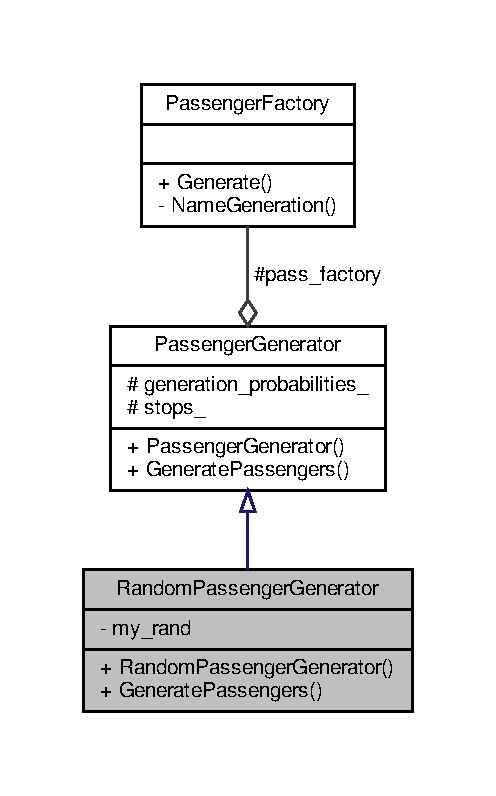
\includegraphics[width=238pt]{classRandomPassengerGenerator__coll__graph}
\end{center}
\end{figure}
\subsection*{Public Member Functions}
\begin{DoxyCompactItemize}
\item 
\hyperlink{classRandomPassengerGenerator_a1be1b4abfe82bfe95eb0a078d9a3342d}{Random\+Passenger\+Generator} (std\+::list$<$ double $>$, std\+::list$<$ \hyperlink{classStop}{Stop} $\ast$$>$)
\begin{DoxyCompactList}\small\item\em Constructs a random passenger generator with a double list and \hyperlink{classStop}{Stop} $\ast$ list. \end{DoxyCompactList}\item 
int \hyperlink{classRandomPassengerGenerator_aba2d80cde33371cf9c3d033f1b8ba6b8}{Generate\+Passengers} () override
\begin{DoxyCompactList}\small\item\em The generate passengers function for \hyperlink{classRandomPassengerGenerator}{Random\+Passenger\+Generator} objects. \end{DoxyCompactList}\end{DoxyCompactItemize}
\subsection*{Static Private Attributes}
\begin{DoxyCompactItemize}
\item 
\mbox{\Hypertarget{classRandomPassengerGenerator_af695eeece3acf5f2e2a7f25f9c46bfbe}\label{classRandomPassengerGenerator_af695eeece3acf5f2e2a7f25f9c46bfbe}} 
static std\+::minstd\+\_\+rand0 {\bfseries my\+\_\+rand}
\end{DoxyCompactItemize}
\subsection*{Additional Inherited Members}


\subsection{Detailed Description}
The main class for the random passenger generator. 

Creates a new instance of a \hyperlink{classRandomPassengerGenerator}{Random\+Passenger\+Generator} object. 

\subsection{Constructor \& Destructor Documentation}
\mbox{\Hypertarget{classRandomPassengerGenerator_a1be1b4abfe82bfe95eb0a078d9a3342d}\label{classRandomPassengerGenerator_a1be1b4abfe82bfe95eb0a078d9a3342d}} 
\index{Random\+Passenger\+Generator@{Random\+Passenger\+Generator}!Random\+Passenger\+Generator@{Random\+Passenger\+Generator}}
\index{Random\+Passenger\+Generator@{Random\+Passenger\+Generator}!Random\+Passenger\+Generator@{Random\+Passenger\+Generator}}
\subsubsection{\texorpdfstring{Random\+Passenger\+Generator()}{RandomPassengerGenerator()}}
{\footnotesize\ttfamily Random\+Passenger\+Generator\+::\+Random\+Passenger\+Generator (\begin{DoxyParamCaption}\item[{std\+::list$<$ double $>$}]{probs,  }\item[{std\+::list$<$ \hyperlink{classStop}{Stop} $\ast$$>$}]{stops }\end{DoxyParamCaption})}



Constructs a random passenger generator with a double list and \hyperlink{classStop}{Stop} $\ast$ list. 


\begin{DoxyParams}[1]{Parameters}
\mbox{\tt in}  & {\em std\+::list$<$double$>$} & holding the probabilities of generation \\
\hline
\mbox{\tt in}  & {\em std\+::list$<$\+Stop} & $\ast$$>$ holding the stops to generate passengers on\\
\hline
\end{DoxyParams}
\begin{DoxyReturn}{Returns}
\hyperlink{classRandomPassengerGenerator}{Random\+Passenger\+Generator} object with double and \hyperlink{classStop}{Stop} $\ast$ list 
\end{DoxyReturn}


\subsection{Member Function Documentation}
\mbox{\Hypertarget{classRandomPassengerGenerator_aba2d80cde33371cf9c3d033f1b8ba6b8}\label{classRandomPassengerGenerator_aba2d80cde33371cf9c3d033f1b8ba6b8}} 
\index{Random\+Passenger\+Generator@{Random\+Passenger\+Generator}!Generate\+Passengers@{Generate\+Passengers}}
\index{Generate\+Passengers@{Generate\+Passengers}!Random\+Passenger\+Generator@{Random\+Passenger\+Generator}}
\subsubsection{\texorpdfstring{Generate\+Passengers()}{GeneratePassengers()}}
{\footnotesize\ttfamily int Random\+Passenger\+Generator\+::\+Generate\+Passengers (\begin{DoxyParamCaption}{ }\end{DoxyParamCaption})\hspace{0.3cm}{\ttfamily [override]}, {\ttfamily [virtual]}}



The generate passengers function for \hyperlink{classRandomPassengerGenerator}{Random\+Passenger\+Generator} objects. 

This function overrides the base class to generate passengers on the \hyperlink{classStop}{Stop} $\ast$ list with the probabilities from the double list.

\begin{DoxyReturn}{Returns}
int number of passengers generated 
\end{DoxyReturn}


Implements \hyperlink{classPassengerGenerator_ad2db96a13b34fcf35977287c06b31d47}{Passenger\+Generator}.



The documentation for this class was generated from the following files\+:\begin{DoxyCompactItemize}
\item 
/home/mamox017/3081\+\_\+f19/repo-\/mamox017/project/src/\hyperlink{random__passenger__generator_8h}{random\+\_\+passenger\+\_\+generator.\+h}\item 
/home/mamox017/3081\+\_\+f19/repo-\/mamox017/project/src/\hyperlink{random__passenger__generator_8cc}{random\+\_\+passenger\+\_\+generator.\+cc}\end{DoxyCompactItemize}

\hypertarget{classRoute}{}\section{Route Class Reference}
\label{classRoute}\index{Route@{Route}}


<<<<<<< HEAD
The main class for a route.  




{\ttfamily \#include $<$route.\+h$>$}



Collaboration diagram for Route\+:\nopagebreak
\begin{figure}[H]
\begin{center}
\leavevmode
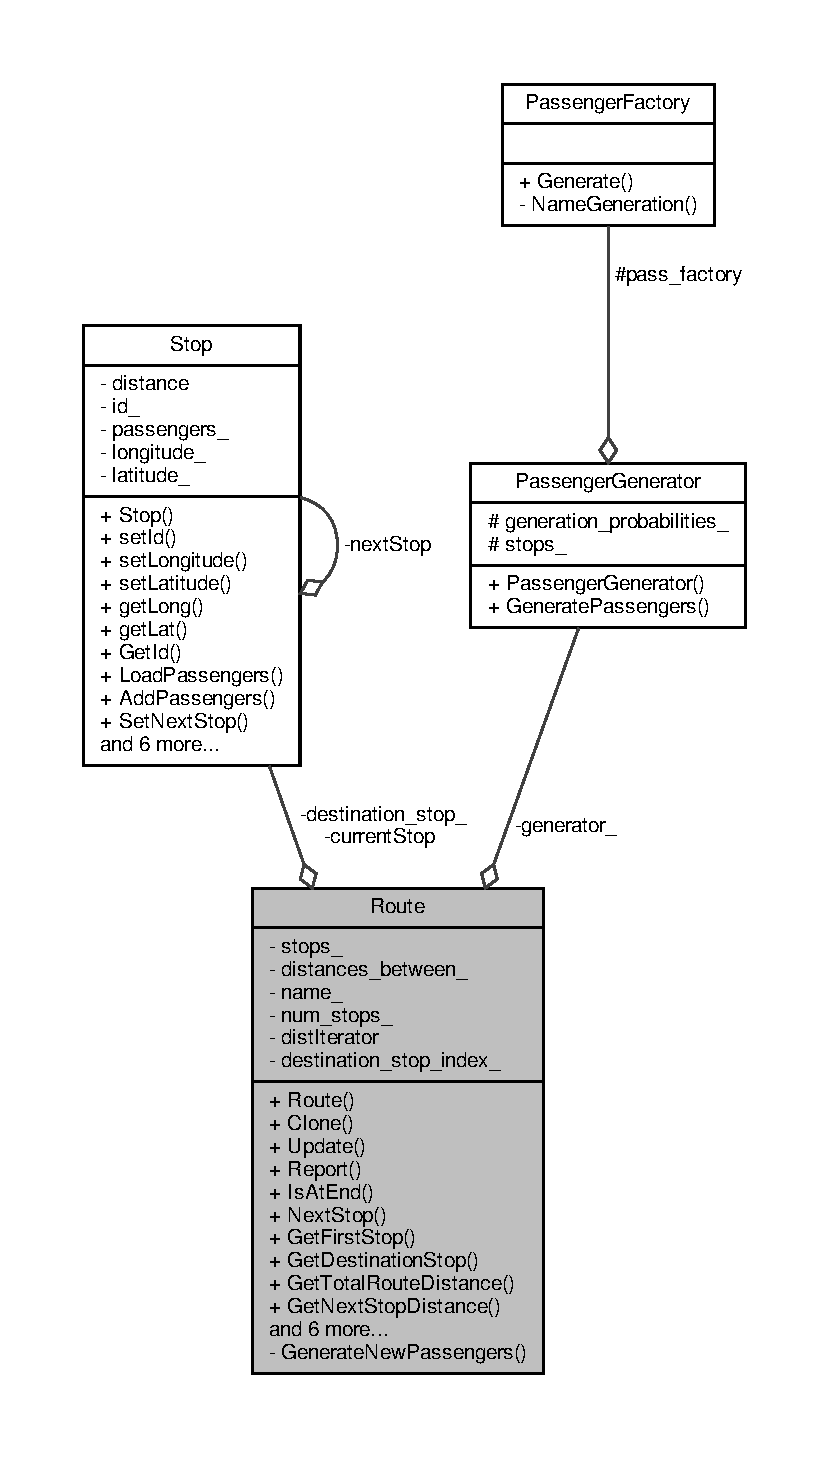
\includegraphics[height=550pt]{classRoute__coll__graph}
=======
Collaboration diagram for Route\+:
\nopagebreak
\begin{figure}[H]
\begin{center}
\leavevmode
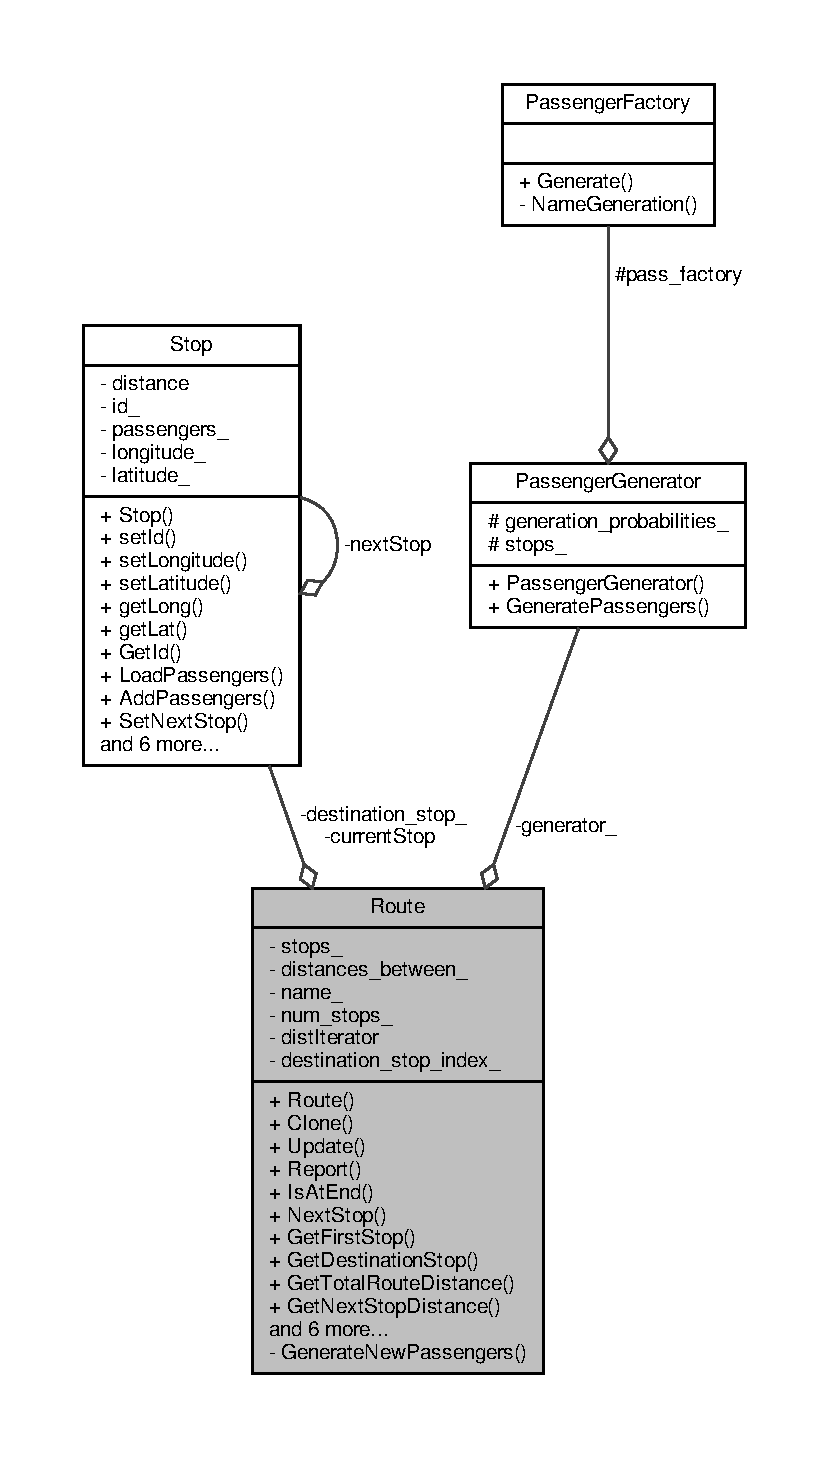
\includegraphics[width=143pt]{classRoute__coll__graph}
>>>>>>> master
\end{center}
\end{figure}
\subsection*{Public Member Functions}
\begin{DoxyCompactItemize}
\item 
<<<<<<< HEAD
\hyperlink{classRoute_ad1bef6c95f3ca3c2713fba850eee9057}{Route} (std\+::string name, \hyperlink{classStop}{Stop} $\ast$$\ast$stops, double $\ast$distances, int num\+\_\+stops, \hyperlink{classPassengerGenerator}{Passenger\+Generator} $\ast$gen)
\begin{DoxyCompactList}\small\item\em Constructs a \hyperlink{classRoute}{Route} with a name, stop list, distance list, number of stops, and a passenger generator. \end{DoxyCompactList}\item 
\hyperlink{classRoute}{Route} $\ast$ \hyperlink{classRoute_a4031b4a218b1530e28dcf5ee5c6fa8e7}{Clone} ()
\begin{DoxyCompactList}\small\item\em Clones a \hyperlink{classRoute}{Route} object, giving it the same attributes. Uses iterator to create deep copies of stop and double lists, while copying over the number of stops and name, as well as pointing to the same generator. \end{DoxyCompactList}\item 
void \hyperlink{classRoute_a7ecf1d4200f5fe110de4a1d9ea9408c3}{Update} ()
\begin{DoxyCompactList}\small\item\em The route updater function for \hyperlink{classRoute}{Route} objects. \end{DoxyCompactList}\item 
void \hyperlink{classRoute_a6115a741ea15af716c1a624627ec954a}{Report} (std\+::ostream \&)
\begin{DoxyCompactList}\small\item\em The report function for \hyperlink{classRoute}{Route} objects. \end{DoxyCompactList}\item 
bool \hyperlink{classRoute_a529ab995aefd1001b250a6c1ccf77892}{Is\+At\+End} () const
\begin{DoxyCompactList}\small\item\em end of route checking function for \hyperlink{classRoute}{Route} objects. \end{DoxyCompactList}\item 
void \hyperlink{classRoute_aefdcf5a8db15f50d840585914744af6f}{Next\+Stop} ()
\begin{DoxyCompactList}\small\item\em The next stop function for \hyperlink{classRoute}{Route} objects. \end{DoxyCompactList}\item 
\hyperlink{classStop}{Stop} $\ast$ \hyperlink{classRoute_aa70ac0596b72df43514f6e3a81552d38}{Get\+First\+Stop} ()
\begin{DoxyCompactList}\small\item\em The get first stop for \hyperlink{classRoute}{Route} objects. \end{DoxyCompactList}\item 
\hyperlink{classStop}{Stop} $\ast$ \hyperlink{classRoute_a44af714485a55a8b6da374399e036cc1}{Get\+Destination\+Stop} () const
\begin{DoxyCompactList}\small\item\em The get destination stop for \hyperlink{classRoute}{Route} objects. \end{DoxyCompactList}\item 
double \hyperlink{classRoute_af4e0add4a9f6b22963398b41313f9e69}{Get\+Total\+Route\+Distance} () const
\begin{DoxyCompactList}\small\item\em The get total route distance for \hyperlink{classRoute}{Route} objects. \end{DoxyCompactList}\item 
double \hyperlink{classRoute_a81b012b2f33a4ead1b084bd3bc308905}{Get\+Next\+Stop\+Distance} ()
\begin{DoxyCompactList}\small\item\em The get next stop distance for \hyperlink{classRoute}{Route} objects. \end{DoxyCompactList}\item 
double \hyperlink{classRoute_a352a82a718bfdec044b114abe332c29f}{Get\+First\+Distance} ()
\begin{DoxyCompactList}\small\item\em The get first stop distance for \hyperlink{classRoute}{Route} objects. \end{DoxyCompactList}\item 
\hyperlink{classStop}{Stop} $\ast$ \hyperlink{classRoute_a1b48fed4a2d4095e1732dcd4c6f3a5a5}{Get\+Last\+Stop} ()
\begin{DoxyCompactList}\small\item\em The get last stop for \hyperlink{classRoute}{Route} objects. \end{DoxyCompactList}\item 
std\+::string \hyperlink{classRoute_a8d05485fe63fbd66fd093d423667ca61}{Get\+Name} ()
\begin{DoxyCompactList}\small\item\em The get name for \hyperlink{classRoute}{Route} objects. \end{DoxyCompactList}\item 
int \hyperlink{classRoute_a2699ed2b1899d8b053cb9363e6dc35b1}{Get\+Num\+Stops} ()
\begin{DoxyCompactList}\small\item\em The get num stops for \hyperlink{classRoute}{Route} objects. \end{DoxyCompactList}\item 
std\+::list$<$ double $>$ \hyperlink{classRoute_a78274b615be2cd45006c5790290eda37}{Get\+Distance\+List} ()
\begin{DoxyCompactList}\small\item\em The get distances list for \hyperlink{classRoute}{Route} objects. \end{DoxyCompactList}\item 
\hyperlink{classPassengerGenerator}{Passenger\+Generator} $\ast$ \hyperlink{classRoute_a31e5860f665b99829a69c3c7adcb465a}{Get\+Generator} ()
\begin{DoxyCompactList}\small\item\em The get generator for \hyperlink{classRoute}{Route} objects. \end{DoxyCompactList}\end{DoxyCompactItemize}
\subsection*{Private Member Functions}
\begin{DoxyCompactItemize}
\item 
\mbox{\Hypertarget{classRoute_a74984ab8d3a054ef2ca58c0dc39a49c7}\label{classRoute_a74984ab8d3a054ef2ca58c0dc39a49c7}} 
int {\bfseries Generate\+New\+Passengers} ()
\end{DoxyCompactItemize}
\subsection*{Private Attributes}
\begin{DoxyCompactItemize}
\item 
\mbox{\Hypertarget{classRoute_abb0d4a5df9055df459fb5f0b7ae2810e}\label{classRoute_abb0d4a5df9055df459fb5f0b7ae2810e}} 
\hyperlink{classPassengerGenerator}{Passenger\+Generator} $\ast$ {\bfseries generator\+\_\+}
\item 
\mbox{\Hypertarget{classRoute_a29357cad3848e8a3ff4dae57610968ee}\label{classRoute_a29357cad3848e8a3ff4dae57610968ee}} 
std\+::list$<$ \hyperlink{classStop}{Stop} $\ast$ $>$ {\bfseries stops\+\_\+}
\item 
\mbox{\Hypertarget{classRoute_a307fe2f7f06105f4f3ae7172264fbcd7}\label{classRoute_a307fe2f7f06105f4f3ae7172264fbcd7}} 
std\+::list$<$ double $>$ {\bfseries distances\+\_\+between\+\_\+}
\item 
\mbox{\Hypertarget{classRoute_a89cf21e933b4599c2fa6dd21728539d9}\label{classRoute_a89cf21e933b4599c2fa6dd21728539d9}} 
std\+::string {\bfseries name\+\_\+}
\item 
\mbox{\Hypertarget{classRoute_ac54981fe7329c32eccbeaea86f7a62f1}\label{classRoute_ac54981fe7329c32eccbeaea86f7a62f1}} 
int {\bfseries num\+\_\+stops\+\_\+}
\item 
\mbox{\Hypertarget{classRoute_aabece44a610bc4a061874026967ffe6a}\label{classRoute_aabece44a610bc4a061874026967ffe6a}} 
std\+::list$<$ double $>$\+::iterator {\bfseries dist\+Iterator}
\item 
\mbox{\Hypertarget{classRoute_aac90998d2c10aa08885436874fb840f2}\label{classRoute_aac90998d2c10aa08885436874fb840f2}} 
int {\bfseries destination\+\_\+stop\+\_\+index\+\_\+}
\item 
\mbox{\Hypertarget{classRoute_a5fea644d7493765558418a8f9fe29aa5}\label{classRoute_a5fea644d7493765558418a8f9fe29aa5}} 
\hyperlink{classStop}{Stop} $\ast$ {\bfseries current\+Stop}
\item 
\mbox{\Hypertarget{classRoute_af702077267c252eae57caa0439b46f94}\label{classRoute_af702077267c252eae57caa0439b46f94}} 
\hyperlink{classStop}{Stop} $\ast$ {\bfseries destination\+\_\+stop\+\_\+}
\end{DoxyCompactItemize}


\subsection{Detailed Description}
The main class for a route. 

Creates a new instance of a \hyperlink{classRoute}{Route} object. 

\subsection{Constructor \& Destructor Documentation}
\mbox{\Hypertarget{classRoute_ad1bef6c95f3ca3c2713fba850eee9057}\label{classRoute_ad1bef6c95f3ca3c2713fba850eee9057}} 
\index{Route@{Route}!Route@{Route}}
\index{Route@{Route}!Route@{Route}}
\subsubsection{\texorpdfstring{Route()}{Route()}}
{\footnotesize\ttfamily Route\+::\+Route (\begin{DoxyParamCaption}\item[{std\+::string}]{name,  }\item[{\hyperlink{classStop}{Stop} $\ast$$\ast$}]{stops,  }\item[{double $\ast$}]{distances,  }\item[{int}]{num\+\_\+stops,  }\item[{\hyperlink{classPassengerGenerator}{Passenger\+Generator} $\ast$}]{gen }\end{DoxyParamCaption})}



Constructs a \hyperlink{classRoute}{Route} with a name, stop list, distance list, number of stops, and a passenger generator. 


\begin{DoxyParams}[1]{Parameters}
\mbox{\tt in}  & {\em std\+::string} & name, label for the route \\
\hline
\mbox{\tt in}  & {\em \hyperlink{classStop}{Stop}} & $\ast$$\ast$ stops, pointer array of \hyperlink{classStop}{Stop} $\ast$ objects in the route \\
\hline
\mbox{\tt in}  & {\em double} & $\ast$ distances, distances between stops on the route \\
\hline
\mbox{\tt in}  & {\em int} & num\+\_\+stops, the number of stops on the route \\
\hline
\mbox{\tt in}  & {\em \hyperlink{classPassengerGenerator}{Passenger\+Generator}} & $\ast$ gen, \hyperlink{classPassengerGenerator}{Passenger\+Generator} object pointer, which will be used to generate passengers on the route.\\
\hline
\end{DoxyParams}
\begin{DoxyReturn}{Returns}
\hyperlink{classRoute}{Route} object with name, stop list, distance list, number of stops, and \hyperlink{classPassengerGenerator}{Passenger\+Generator} 
\end{DoxyReturn}


\subsection{Member Function Documentation}
\mbox{\Hypertarget{classRoute_a4031b4a218b1530e28dcf5ee5c6fa8e7}\label{classRoute_a4031b4a218b1530e28dcf5ee5c6fa8e7}} 
\index{Route@{Route}!Clone@{Clone}}
\index{Clone@{Clone}!Route@{Route}}
\subsubsection{\texorpdfstring{Clone()}{Clone()}}
{\footnotesize\ttfamily \hyperlink{classRoute}{Route} $\ast$ Route\+::\+Clone (\begin{DoxyParamCaption}{ }\end{DoxyParamCaption})}



Clones a \hyperlink{classRoute}{Route} object, giving it the same attributes. Uses iterator to create deep copies of stop and double lists, while copying over the number of stops and name, as well as pointing to the same generator. 

\begin{DoxyReturn}{Returns}
\hyperlink{classRoute}{Route} $\ast$ copy of \hyperlink{classRoute}{Route} object 
\end{DoxyReturn}
\mbox{\Hypertarget{classRoute_a44af714485a55a8b6da374399e036cc1}\label{classRoute_a44af714485a55a8b6da374399e036cc1}} 
\index{Route@{Route}!Get\+Destination\+Stop@{Get\+Destination\+Stop}}
\index{Get\+Destination\+Stop@{Get\+Destination\+Stop}!Route@{Route}}
\subsubsection{\texorpdfstring{Get\+Destination\+Stop()}{GetDestinationStop()}}
{\footnotesize\ttfamily \hyperlink{classStop}{Stop} $\ast$ Route\+::\+Get\+Destination\+Stop (\begin{DoxyParamCaption}{ }\end{DoxyParamCaption}) const}



The get destination stop for \hyperlink{classRoute}{Route} objects. 

This function accesses destination\+\_\+stop\+\_\+ member variable.

\begin{DoxyReturn}{Returns}
\hyperlink{classStop}{Stop} $\ast$ object of next destination stop on the route 
\end{DoxyReturn}
\mbox{\Hypertarget{classRoute_a78274b615be2cd45006c5790290eda37}\label{classRoute_a78274b615be2cd45006c5790290eda37}} 
\index{Route@{Route}!Get\+Distance\+List@{Get\+Distance\+List}}
\index{Get\+Distance\+List@{Get\+Distance\+List}!Route@{Route}}
\subsubsection{\texorpdfstring{Get\+Distance\+List()}{GetDistanceList()}}
{\footnotesize\ttfamily std\+::list$<$ double $>$ Route\+::\+Get\+Distance\+List (\begin{DoxyParamCaption}{ }\end{DoxyParamCaption})}



The get distances list for \hyperlink{classRoute}{Route} objects. 

This accessor retrieves the route stop distances for testing purposes.

\begin{DoxyReturn}{Returns}
std\+::list$<$double$>$ list of the distances between stops on route 
\end{DoxyReturn}
\mbox{\Hypertarget{classRoute_a352a82a718bfdec044b114abe332c29f}\label{classRoute_a352a82a718bfdec044b114abe332c29f}} 
\index{Route@{Route}!Get\+First\+Distance@{Get\+First\+Distance}}
\index{Get\+First\+Distance@{Get\+First\+Distance}!Route@{Route}}
\subsubsection{\texorpdfstring{Get\+First\+Distance()}{GetFirstDistance()}}
{\footnotesize\ttfamily double Route\+::\+Get\+First\+Distance (\begin{DoxyParamCaption}{ }\end{DoxyParamCaption})}



The get first stop distance for \hyperlink{classRoute}{Route} objects. 

This function uses .front() on the list of distances\+\_\+between\+\_\+ to get the first distance away on the \hyperlink{classRoute}{Route}.

\begin{DoxyReturn}{Returns}
double distance away of first stop 
\end{DoxyReturn}
\mbox{\Hypertarget{classRoute_aa70ac0596b72df43514f6e3a81552d38}\label{classRoute_aa70ac0596b72df43514f6e3a81552d38}} 
\index{Route@{Route}!Get\+First\+Stop@{Get\+First\+Stop}}
\index{Get\+First\+Stop@{Get\+First\+Stop}!Route@{Route}}
\subsubsection{\texorpdfstring{Get\+First\+Stop()}{GetFirstStop()}}
{\footnotesize\ttfamily \hyperlink{classStop}{Stop} $\ast$ Route\+::\+Get\+First\+Stop (\begin{DoxyParamCaption}{ }\end{DoxyParamCaption})}



The get first stop for \hyperlink{classRoute}{Route} objects. 

This function accesses the first stop on the \hyperlink{classRoute}{Route} by using .front() on the stop list. Also sets destination\+\_\+stop to second stop.

\begin{DoxyReturn}{Returns}
\hyperlink{classStop}{Stop} $\ast$ object of first stop on the route 
\end{DoxyReturn}
\mbox{\Hypertarget{classRoute_a31e5860f665b99829a69c3c7adcb465a}\label{classRoute_a31e5860f665b99829a69c3c7adcb465a}} 
\index{Route@{Route}!Get\+Generator@{Get\+Generator}}
\index{Get\+Generator@{Get\+Generator}!Route@{Route}}
\subsubsection{\texorpdfstring{Get\+Generator()}{GetGenerator()}}
{\footnotesize\ttfamily \hyperlink{classPassengerGenerator}{Passenger\+Generator} $\ast$ Route\+::\+Get\+Generator (\begin{DoxyParamCaption}{ }\end{DoxyParamCaption})}



The get generator for \hyperlink{classRoute}{Route} objects. 

This accessor retrieves the \hyperlink{classPassengerGenerator}{Passenger\+Generator} for testing purposes.

\begin{DoxyReturn}{Returns}
\hyperlink{classPassengerGenerator}{Passenger\+Generator} generator of the route 
\end{DoxyReturn}
\mbox{\Hypertarget{classRoute_a1b48fed4a2d4095e1732dcd4c6f3a5a5}\label{classRoute_a1b48fed4a2d4095e1732dcd4c6f3a5a5}} 
\index{Route@{Route}!Get\+Last\+Stop@{Get\+Last\+Stop}}
\index{Get\+Last\+Stop@{Get\+Last\+Stop}!Route@{Route}}
\subsubsection{\texorpdfstring{Get\+Last\+Stop()}{GetLastStop()}}
{\footnotesize\ttfamily \hyperlink{classStop}{Stop} $\ast$ Route\+::\+Get\+Last\+Stop (\begin{DoxyParamCaption}{ }\end{DoxyParamCaption})}



The get last stop for \hyperlink{classRoute}{Route} objects. 

This function uses .back() on the stop list to retrieve the last stop on the \hyperlink{classRoute}{Route}

\begin{DoxyReturn}{Returns}
\hyperlink{classStop}{Stop} $\ast$ last stop on the route 
\end{DoxyReturn}
\mbox{\Hypertarget{classRoute_a8d05485fe63fbd66fd093d423667ca61}\label{classRoute_a8d05485fe63fbd66fd093d423667ca61}} 
\index{Route@{Route}!Get\+Name@{Get\+Name}}
\index{Get\+Name@{Get\+Name}!Route@{Route}}
\subsubsection{\texorpdfstring{Get\+Name()}{GetName()}}
{\footnotesize\ttfamily std\+::string Route\+::\+Get\+Name (\begin{DoxyParamCaption}{ }\end{DoxyParamCaption})}



The get name for \hyperlink{classRoute}{Route} objects. 

This accessor retrieves the route name\+\_\+ for testing purposes.

\begin{DoxyReturn}{Returns}
std\+::name name of the route 
\end{DoxyReturn}
\mbox{\Hypertarget{classRoute_a81b012b2f33a4ead1b084bd3bc308905}\label{classRoute_a81b012b2f33a4ead1b084bd3bc308905}} 
\index{Route@{Route}!Get\+Next\+Stop\+Distance@{Get\+Next\+Stop\+Distance}}
\index{Get\+Next\+Stop\+Distance@{Get\+Next\+Stop\+Distance}!Route@{Route}}
\subsubsection{\texorpdfstring{Get\+Next\+Stop\+Distance()}{GetNextStopDistance()}}
{\footnotesize\ttfamily double Route\+::\+Get\+Next\+Stop\+Distance (\begin{DoxyParamCaption}{ }\end{DoxyParamCaption})}



The get next stop distance for \hyperlink{classRoute}{Route} objects. 

This function uses an accessor on the destination\+\_\+stop\+\_\+ to retrieve its distance away.

\begin{DoxyReturn}{Returns}
double distance away of next stop 
\end{DoxyReturn}
\mbox{\Hypertarget{classRoute_a2699ed2b1899d8b053cb9363e6dc35b1}\label{classRoute_a2699ed2b1899d8b053cb9363e6dc35b1}} 
\index{Route@{Route}!Get\+Num\+Stops@{Get\+Num\+Stops}}
\index{Get\+Num\+Stops@{Get\+Num\+Stops}!Route@{Route}}
\subsubsection{\texorpdfstring{Get\+Num\+Stops()}{GetNumStops()}}
{\footnotesize\ttfamily int Route\+::\+Get\+Num\+Stops (\begin{DoxyParamCaption}{ }\end{DoxyParamCaption})}



The get num stops for \hyperlink{classRoute}{Route} objects. 

This accessor retrieves the num\+\_\+stops\+\_\+ for testing purposes.

\begin{DoxyReturn}{Returns}
int num\+\_\+stops\+\_\+ of the route 
\end{DoxyReturn}
\mbox{\Hypertarget{classRoute_af4e0add4a9f6b22963398b41313f9e69}\label{classRoute_af4e0add4a9f6b22963398b41313f9e69}} 
\index{Route@{Route}!Get\+Total\+Route\+Distance@{Get\+Total\+Route\+Distance}}
\index{Get\+Total\+Route\+Distance@{Get\+Total\+Route\+Distance}!Route@{Route}}
\subsubsection{\texorpdfstring{Get\+Total\+Route\+Distance()}{GetTotalRouteDistance()}}
{\footnotesize\ttfamily double Route\+::\+Get\+Total\+Route\+Distance (\begin{DoxyParamCaption}{ }\end{DoxyParamCaption}) const}



The get total route distance for \hyperlink{classRoute}{Route} objects. 

This function iterates through the double list of distances and adds them to a running sum.

\begin{DoxyReturn}{Returns}
double sum of all distances on the route 
\end{DoxyReturn}
\mbox{\Hypertarget{classRoute_a529ab995aefd1001b250a6c1ccf77892}\label{classRoute_a529ab995aefd1001b250a6c1ccf77892}} 
\index{Route@{Route}!Is\+At\+End@{Is\+At\+End}}
\index{Is\+At\+End@{Is\+At\+End}!Route@{Route}}
\subsubsection{\texorpdfstring{Is\+At\+End()}{IsAtEnd()}}
{\footnotesize\ttfamily bool Route\+::\+Is\+At\+End (\begin{DoxyParamCaption}{ }\end{DoxyParamCaption}) const}



end of route checking function for \hyperlink{classRoute}{Route} objects. 

This function checks if the route is at the end by examining whether or not the current\+Stop is the same as the back of the stop list.

\begin{DoxyReturn}{Returns}
bool object that is true if at end and false if not at end of route 
\end{DoxyReturn}
\mbox{\Hypertarget{classRoute_aefdcf5a8db15f50d840585914744af6f}\label{classRoute_aefdcf5a8db15f50d840585914744af6f}} 
\index{Route@{Route}!Next\+Stop@{Next\+Stop}}
\index{Next\+Stop@{Next\+Stop}!Route@{Route}}
\subsubsection{\texorpdfstring{Next\+Stop()}{NextStop()}}
{\footnotesize\ttfamily void Route\+::\+Next\+Stop (\begin{DoxyParamCaption}{ }\end{DoxyParamCaption})}



The next stop function for \hyperlink{classRoute}{Route} objects. 

This function changes current\+Stop to the destination\+\_\+stop\+\_\+ and changes the destination\+\_\+stop\+\_\+ to next stop. Also increments destination\+\_\+stop\+\_\+index\+\_\+.

\begin{DoxyReturn}{Returns}
void 
\end{DoxyReturn}
\mbox{\Hypertarget{classRoute_a6115a741ea15af716c1a624627ec954a}\label{classRoute_a6115a741ea15af716c1a624627ec954a}} 
\index{Route@{Route}!Report@{Report}}
\index{Report@{Report}!Route@{Route}}
\subsubsection{\texorpdfstring{Report()}{Report()}}
{\footnotesize\ttfamily void Route\+::\+Report (\begin{DoxyParamCaption}\item[{std\+::ostream \&}]{o }\end{DoxyParamCaption})}



The report function for \hyperlink{classRoute}{Route} objects. 

This function reports the \hyperlink{classRoute}{Route}\textquotesingle{}s attributes to a given output stream.


\begin{DoxyParams}[1]{Parameters}
\mbox{\tt in}  & {\em std\+::ostream\&} & o, the output stream to which the information is sent.\\
\hline
\end{DoxyParams}
\begin{DoxyReturn}{Returns}
void 
\end{DoxyReturn}
\mbox{\Hypertarget{classRoute_a7ecf1d4200f5fe110de4a1d9ea9408c3}\label{classRoute_a7ecf1d4200f5fe110de4a1d9ea9408c3}} 
\index{Route@{Route}!Update@{Update}}
\index{Update@{Update}!Route@{Route}}
\subsubsection{\texorpdfstring{Update()}{Update()}}
{\footnotesize\ttfamily void Route\+::\+Update (\begin{DoxyParamCaption}{ }\end{DoxyParamCaption})}



The route updater function for \hyperlink{classRoute}{Route} objects. 

This function updates the \hyperlink{classRoute}{Route} by updating all the stops on the route and calling for the generation of passengers.

\begin{DoxyReturn}{Returns}
void 
\end{DoxyReturn}


=======
\mbox{\Hypertarget{classRoute_a10f76d08631603cafdc7561522b2f436}\label{classRoute_a10f76d08631603cafdc7561522b2f436}} 
{\bfseries Route} (std\+::string name, \hyperlink{classStop}{Stop} $\ast$$\ast$stops, double $\ast$distances, int num\+\_\+stops)
\item 
\mbox{\Hypertarget{classRoute_a7ecf1d4200f5fe110de4a1d9ea9408c3}\label{classRoute_a7ecf1d4200f5fe110de4a1d9ea9408c3}} 
void {\bfseries Update} ()
\item 
\mbox{\Hypertarget{classRoute_a73b08f4521e0cd74c62cf748ee245db4}\label{classRoute_a73b08f4521e0cd74c62cf748ee245db4}} 
void {\bfseries Report} ()
\end{DoxyCompactItemize}


>>>>>>> master
The documentation for this class was generated from the following files\+:\begin{DoxyCompactItemize}
\item 
/home/mamox017/3081\+\_\+f19/repo-\/mamox017/project/src/\hyperlink{route_8h}{route.\+h}\item 
/home/mamox017/3081\+\_\+f19/repo-\/mamox017/project/src/route.\+cc\end{DoxyCompactItemize}

\hypertarget{classSimulator}{}\section{Simulator Class Reference}
\label{classSimulator}\index{Simulator@{Simulator}}


The main class for the simulator.  




{\ttfamily \#include $<$simulator.\+h$>$}



Inheritance diagram for Simulator\+:\nopagebreak
\begin{figure}[H]
\begin{center}
\leavevmode
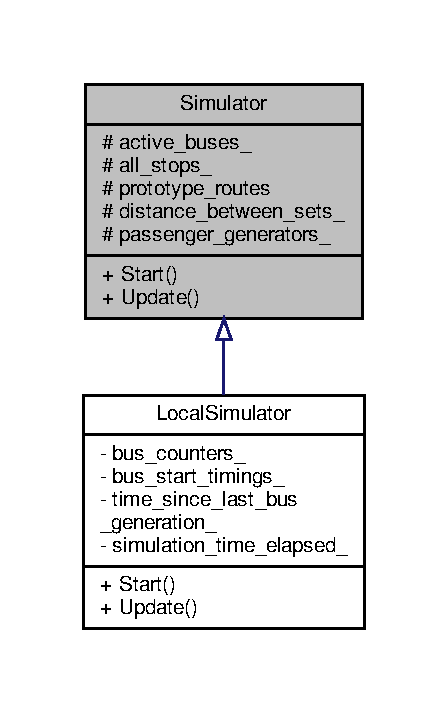
\includegraphics[width=215pt]{classSimulator__inherit__graph}
\end{center}
\end{figure}


Collaboration diagram for Simulator\+:\nopagebreak
\begin{figure}[H]
\begin{center}
\leavevmode
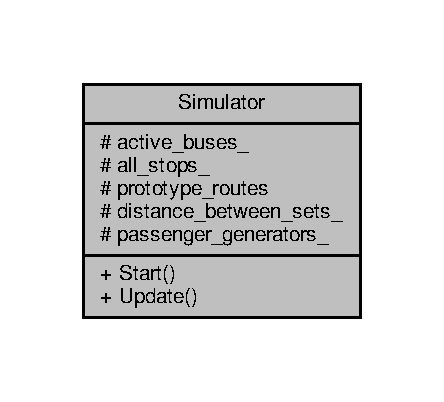
\includegraphics[width=213pt]{classSimulator__coll__graph}
\end{center}
\end{figure}
\subsection*{Public Member Functions}
\begin{DoxyCompactItemize}
\item 
virtual bool \hyperlink{classSimulator_a0db68bef442ba6061a5f38189bbe3512}{Start} ()=0
\begin{DoxyCompactList}\small\item\em The Start function for \hyperlink{classSimulator}{Simulator} objects. \end{DoxyCompactList}\item 
virtual bool \hyperlink{classSimulator_a7a5a1cbfa1e0cf9b82fe9d2e4b3b80ae}{Update} ()=0
\begin{DoxyCompactList}\small\item\em The Update function for \hyperlink{classSimulator}{Simulator} objects. \end{DoxyCompactList}\end{DoxyCompactItemize}
\subsection*{Protected Attributes}
\begin{DoxyCompactItemize}
\item 
\mbox{\Hypertarget{classSimulator_a2936ff199db47fac93a4ca2970a8bf9a}\label{classSimulator_a2936ff199db47fac93a4ca2970a8bf9a}} 
std\+::list$<$ \hyperlink{classBus}{Bus} $\ast$ $>$ {\bfseries active\+\_\+buses\+\_\+}
\item 
\mbox{\Hypertarget{classSimulator_aa5539319a6b4a70c2d0c6f6220fe44c7}\label{classSimulator_aa5539319a6b4a70c2d0c6f6220fe44c7}} 
std\+::list$<$ \hyperlink{classStop}{Stop} $\ast$ $>$ {\bfseries all\+\_\+stops\+\_\+}
\item 
\mbox{\Hypertarget{classSimulator_a5be4c046d8654aa28b37308f581c3fc9}\label{classSimulator_a5be4c046d8654aa28b37308f581c3fc9}} 
std\+::vector$<$ \hyperlink{classRoute}{Route} $\ast$ $>$ {\bfseries prototype\+\_\+routes}
\item 
\mbox{\Hypertarget{classSimulator_aa14b28ce4f5c0fa6f9e96f9e3b9aae73}\label{classSimulator_aa14b28ce4f5c0fa6f9e96f9e3b9aae73}} 
std\+::vector$<$ double $\ast$ $>$ {\bfseries distance\+\_\+between\+\_\+sets\+\_\+}
\item 
\mbox{\Hypertarget{classSimulator_a666884fa56160538fb7ceac476aedd44}\label{classSimulator_a666884fa56160538fb7ceac476aedd44}} 
std\+::vector$<$ \hyperlink{classPassengerGenerator}{Passenger\+Generator} $\ast$ $>$ {\bfseries passenger\+\_\+generators\+\_\+}
\end{DoxyCompactItemize}


\subsection{Detailed Description}
The main class for the simulator. 

Creates a new instance of a \hyperlink{classSimulator}{Simulator} object. 

\subsection{Member Function Documentation}
\mbox{\Hypertarget{classSimulator_a0db68bef442ba6061a5f38189bbe3512}\label{classSimulator_a0db68bef442ba6061a5f38189bbe3512}} 
\index{Simulator@{Simulator}!Start@{Start}}
\index{Start@{Start}!Simulator@{Simulator}}
\subsubsection{\texorpdfstring{Start()}{Start()}}
{\footnotesize\ttfamily virtual bool Simulator\+::\+Start (\begin{DoxyParamCaption}{ }\end{DoxyParamCaption})\hspace{0.3cm}{\ttfamily [pure virtual]}}



The Start function for \hyperlink{classSimulator}{Simulator} objects. 

This pure virtual function is to be used by inheriting classes to start a simulation of given situations.

\begin{DoxyReturn}{Returns}
bool = 0, indicates whether simulation successfully starts 
\end{DoxyReturn}


Implemented in \hyperlink{classLocalSimulator_a380634942668855dd1da8276b270b362}{Local\+Simulator}.

\mbox{\Hypertarget{classSimulator_a7a5a1cbfa1e0cf9b82fe9d2e4b3b80ae}\label{classSimulator_a7a5a1cbfa1e0cf9b82fe9d2e4b3b80ae}} 
\index{Simulator@{Simulator}!Update@{Update}}
\index{Update@{Update}!Simulator@{Simulator}}
\subsubsection{\texorpdfstring{Update()}{Update()}}
{\footnotesize\ttfamily virtual bool Simulator\+::\+Update (\begin{DoxyParamCaption}{ }\end{DoxyParamCaption})\hspace{0.3cm}{\ttfamily [pure virtual]}}



The Update function for \hyperlink{classSimulator}{Simulator} objects. 

This pure virtual function is to be used by inheriting classes to update a simulation.

\begin{DoxyReturn}{Returns}
bool = 0, indicates whether simulation successfully updates 
\end{DoxyReturn}


Implemented in \hyperlink{classLocalSimulator_ac98ba1a401ad204dd5169934adb02684}{Local\+Simulator}.



The documentation for this class was generated from the following file\+:\begin{DoxyCompactItemize}
\item 
/home/mamox017/3081\+\_\+f19/repo-\/mamox017/project/src/\hyperlink{simulator_8h}{simulator.\+h}\end{DoxyCompactItemize}

\hypertarget{classStop}{}\section{Stop Class Reference}
\label{classStop}\index{Stop@{Stop}}


<<<<<<< HEAD
The main class for a stop.  




{\ttfamily \#include $<$stop.\+h$>$}



Collaboration diagram for Stop\+:\nopagebreak
\begin{figure}[H]
\begin{center}
\leavevmode
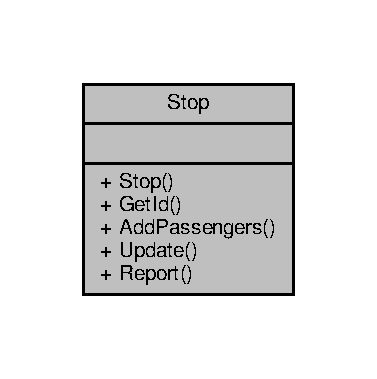
\includegraphics[width=248pt]{classStop__coll__graph}
=======
Collaboration diagram for Stop\+:
\nopagebreak
\begin{figure}[H]
\begin{center}
\leavevmode
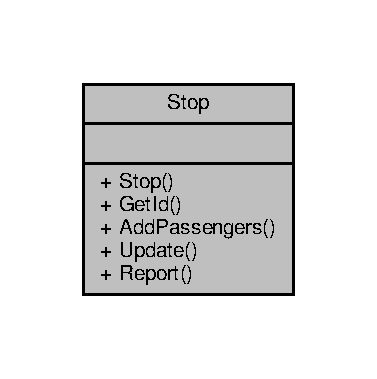
\includegraphics[width=181pt]{classStop__coll__graph}
>>>>>>> master
\end{center}
\end{figure}
\subsection*{Public Member Functions}
\begin{DoxyCompactItemize}
\item 
<<<<<<< HEAD
\hyperlink{classStop_a59d881f072b1cf89512bb15a51ffc773}{Stop} (int, double=44.\+973723, double=-\/93.\+235365)
\begin{DoxyCompactList}\small\item\em Constructs a \hyperlink{classStop}{Stop} with an id, longitude and latitude. \end{DoxyCompactList}\item 
void \hyperlink{classStop_a936324668d7b9f5edfbe4531cf244608}{set\+Id} (int i)
\begin{DoxyCompactList}\small\item\em The stop set id function for \hyperlink{classStop}{Stop} objects. \end{DoxyCompactList}\item 
void \hyperlink{classStop_a26866e7dfd469467c67d4176693b53c7}{set\+Longitude} (double l)
\begin{DoxyCompactList}\small\item\em The stop set longitude function for \hyperlink{classStop}{Stop} objects. \end{DoxyCompactList}\item 
void \hyperlink{classStop_ad70323088d687724e6eaad1eb723061f}{set\+Latitude} (double lat)
\begin{DoxyCompactList}\small\item\em The stop set latitude function for \hyperlink{classStop}{Stop} objects. \end{DoxyCompactList}\item 
double \hyperlink{classStop_aea4bfbf489a3a61ecb104e9aa9f613c4}{get\+Long} ()
\begin{DoxyCompactList}\small\item\em The stop get longitude function for \hyperlink{classStop}{Stop} objects. \end{DoxyCompactList}\item 
double \hyperlink{classStop_ad26553052a5ee0c478f4988ec51236d9}{get\+Lat} ()
\begin{DoxyCompactList}\small\item\em The stop get id function for \hyperlink{classStop}{Stop} objects. \end{DoxyCompactList}\item 
int \hyperlink{classStop_a2f3b845d5a338f197226c90696314904}{Get\+Id} () const
\begin{DoxyCompactList}\small\item\em The stop get id function for \hyperlink{classStop}{Stop} objects. \end{DoxyCompactList}\item 
int \hyperlink{classStop_a02c6dcba2b6de5fdd008cf623f19bf7c}{Load\+Passengers} (\hyperlink{classBus}{Bus} $\ast$)
\begin{DoxyCompactList}\small\item\em The load passengers function for \hyperlink{classStop}{Stop} objects. \end{DoxyCompactList}\item 
int \hyperlink{classStop_a20a8b6035679d92a7a838a03a102bcd1}{Add\+Passengers} (\hyperlink{classPassenger}{Passenger} $\ast$)
\begin{DoxyCompactList}\small\item\em The add passengers function for \hyperlink{classStop}{Stop} objects. \end{DoxyCompactList}\item 
void \hyperlink{classStop_a7e39a7138f5bcf8f144155de7b1ae1aa}{Set\+Next\+Stop} (\hyperlink{classStop}{Stop} $\ast$next)
\begin{DoxyCompactList}\small\item\em The set next stop function for \hyperlink{classStop}{Stop} objects. \end{DoxyCompactList}\item 
\hyperlink{classStop}{Stop} $\ast$ \hyperlink{classStop_a195566d0fb9cc1bcc8929cffd5602052}{Get\+Next\+Stop} ()
\begin{DoxyCompactList}\small\item\em The get next stop for \hyperlink{classStop}{Stop} objects. \end{DoxyCompactList}\item 
double \hyperlink{classStop_a75185ff04f33083582c98230fc3a6df4}{get\+Distance} ()
\begin{DoxyCompactList}\small\item\em The get distance for \hyperlink{classStop}{Stop} objects. \end{DoxyCompactList}\item 
void \hyperlink{classStop_af26acbcbca66d3a36ce01bc662e2e892}{set\+Distance} (double dis)
\begin{DoxyCompactList}\small\item\em The set distance for \hyperlink{classStop}{Stop} objects. \end{DoxyCompactList}\item 
void \hyperlink{classStop_aa373ae256ce6bc01ef13e876dfdec5bd}{Update} ()
\begin{DoxyCompactList}\small\item\em The stop updater function for \hyperlink{classStop}{Stop} objects. \end{DoxyCompactList}\item 
void \hyperlink{classStop_a8e286b7cca2dce6977ebda6f01805d94}{Report} (std\+::ostream \&) const
\begin{DoxyCompactList}\small\item\em The report function for \hyperlink{classStop}{Stop} objects. \end{DoxyCompactList}\item 
std\+::list$<$ \hyperlink{classPassenger}{Passenger} $\ast$ $>$ \hyperlink{classStop_a57c093d381664512dd576cf02a88bea6}{Get\+Passenger\+List} ()
\begin{DoxyCompactList}\small\item\em The get passenger list for \hyperlink{classStop}{Stop} objects. \end{DoxyCompactList}\end{DoxyCompactItemize}
\subsection*{Private Attributes}
\begin{DoxyCompactItemize}
\item 
\mbox{\Hypertarget{classStop_aa687fb4e9e5876af53b0f40459ae9d49}\label{classStop_aa687fb4e9e5876af53b0f40459ae9d49}} 
\hyperlink{classStop}{Stop} $\ast$ {\bfseries next\+Stop}
\item 
\mbox{\Hypertarget{classStop_a62a29cc045a4e927a367eee662cc5d2d}\label{classStop_a62a29cc045a4e927a367eee662cc5d2d}} 
double {\bfseries distance}
\item 
\mbox{\Hypertarget{classStop_a71becdbe8bf6168f72f9c8ea2b3dc0c4}\label{classStop_a71becdbe8bf6168f72f9c8ea2b3dc0c4}} 
int {\bfseries id\+\_\+}
\item 
\mbox{\Hypertarget{classStop_a1e75327b0aadd184120bf6a85eb641fa}\label{classStop_a1e75327b0aadd184120bf6a85eb641fa}} 
std\+::list$<$ \hyperlink{classPassenger}{Passenger} $\ast$ $>$ {\bfseries passengers\+\_\+}
\item 
\mbox{\Hypertarget{classStop_a6fbad9a47cf803d0f43a60d3b954505c}\label{classStop_a6fbad9a47cf803d0f43a60d3b954505c}} 
double {\bfseries longitude\+\_\+}
\item 
\mbox{\Hypertarget{classStop_a4314074f0842c7e2483d341061bdb293}\label{classStop_a4314074f0842c7e2483d341061bdb293}} 
double {\bfseries latitude\+\_\+}
\end{DoxyCompactItemize}


\subsection{Detailed Description}
The main class for a stop. 

Creates a new instance of a \hyperlink{classStop}{Stop} object. 

\subsection{Constructor \& Destructor Documentation}
\mbox{\Hypertarget{classStop_a59d881f072b1cf89512bb15a51ffc773}\label{classStop_a59d881f072b1cf89512bb15a51ffc773}} 
\index{Stop@{Stop}!Stop@{Stop}}
\index{Stop@{Stop}!Stop@{Stop}}
\subsubsection{\texorpdfstring{Stop()}{Stop()}}
{\footnotesize\ttfamily Stop\+::\+Stop (\begin{DoxyParamCaption}\item[{int}]{id,  }\item[{double}]{longitude = {\ttfamily 44.973723},  }\item[{double}]{latitude = {\ttfamily -\/93.235365} }\end{DoxyParamCaption})\hspace{0.3cm}{\ttfamily [explicit]}}



Constructs a \hyperlink{classStop}{Stop} with an id, longitude and latitude. 

This function is explicit.


\begin{DoxyParams}[1]{Parameters}
\mbox{\tt in}  & {\em int} & holding an id number \\
\hline
\mbox{\tt in}  & {\em double} & holding the longitude of the stop \\
\hline
\mbox{\tt in}  & {\em double} & holding the latitude of the stop\\
\hline
\end{DoxyParams}
\begin{DoxyReturn}{Returns}
\hyperlink{classStop}{Stop} object with id, longitude and latitude 
\end{DoxyReturn}


\subsection{Member Function Documentation}
\mbox{\Hypertarget{classStop_a20a8b6035679d92a7a838a03a102bcd1}\label{classStop_a20a8b6035679d92a7a838a03a102bcd1}} 
\index{Stop@{Stop}!Add\+Passengers@{Add\+Passengers}}
\index{Add\+Passengers@{Add\+Passengers}!Stop@{Stop}}
\subsubsection{\texorpdfstring{Add\+Passengers()}{AddPassengers()}}
{\footnotesize\ttfamily int Stop\+::\+Add\+Passengers (\begin{DoxyParamCaption}\item[{\hyperlink{classPassenger}{Passenger} $\ast$}]{pass }\end{DoxyParamCaption})}



The add passengers function for \hyperlink{classStop}{Stop} objects. 


\begin{DoxyParams}[1]{Parameters}
\mbox{\tt in}  & {\em \hyperlink{classPassenger}{Passenger}} & $\ast$ pointer to a passenger to add to stop. Added to stop list by .push\+\_\+back().\\
\hline
\end{DoxyParams}
\begin{DoxyReturn}{Returns}
int 0 for success 
\end{DoxyReturn}
\mbox{\Hypertarget{classStop_a75185ff04f33083582c98230fc3a6df4}\label{classStop_a75185ff04f33083582c98230fc3a6df4}} 
\index{Stop@{Stop}!get\+Distance@{get\+Distance}}
\index{get\+Distance@{get\+Distance}!Stop@{Stop}}
\subsubsection{\texorpdfstring{get\+Distance()}{getDistance()}}
{\footnotesize\ttfamily double Stop\+::get\+Distance (\begin{DoxyParamCaption}{ }\end{DoxyParamCaption})}



The get distance for \hyperlink{classStop}{Stop} objects. 

This function accesses the distance member variable.

\begin{DoxyReturn}{Returns}
double distance of next stop 
\end{DoxyReturn}
\mbox{\Hypertarget{classStop_a2f3b845d5a338f197226c90696314904}\label{classStop_a2f3b845d5a338f197226c90696314904}} 
\index{Stop@{Stop}!Get\+Id@{Get\+Id}}
\index{Get\+Id@{Get\+Id}!Stop@{Stop}}
\subsubsection{\texorpdfstring{Get\+Id()}{GetId()}}
{\footnotesize\ttfamily int Stop\+::\+Get\+Id (\begin{DoxyParamCaption}{ }\end{DoxyParamCaption}) const}



The stop get id function for \hyperlink{classStop}{Stop} objects. 

This function accesses the stop\textquotesingle{}s id.

\begin{DoxyReturn}{Returns}
int id of the stop 
\end{DoxyReturn}
\mbox{\Hypertarget{classStop_ad26553052a5ee0c478f4988ec51236d9}\label{classStop_ad26553052a5ee0c478f4988ec51236d9}} 
\index{Stop@{Stop}!get\+Lat@{get\+Lat}}
\index{get\+Lat@{get\+Lat}!Stop@{Stop}}
\subsubsection{\texorpdfstring{get\+Lat()}{getLat()}}
{\footnotesize\ttfamily double Stop\+::get\+Lat (\begin{DoxyParamCaption}{ }\end{DoxyParamCaption})}



The stop get id function for \hyperlink{classStop}{Stop} objects. 

This function accesses the stop\textquotesingle{}s latitude.

\begin{DoxyReturn}{Returns}
double latitude of the stop 
\end{DoxyReturn}
\mbox{\Hypertarget{classStop_aea4bfbf489a3a61ecb104e9aa9f613c4}\label{classStop_aea4bfbf489a3a61ecb104e9aa9f613c4}} 
\index{Stop@{Stop}!get\+Long@{get\+Long}}
\index{get\+Long@{get\+Long}!Stop@{Stop}}
\subsubsection{\texorpdfstring{get\+Long()}{getLong()}}
{\footnotesize\ttfamily double Stop\+::get\+Long (\begin{DoxyParamCaption}{ }\end{DoxyParamCaption})}



The stop get longitude function for \hyperlink{classStop}{Stop} objects. 

This function accesses the stop\textquotesingle{}s longitude.

\begin{DoxyReturn}{Returns}
double longitude of the stop 
\end{DoxyReturn}
\mbox{\Hypertarget{classStop_a195566d0fb9cc1bcc8929cffd5602052}\label{classStop_a195566d0fb9cc1bcc8929cffd5602052}} 
\index{Stop@{Stop}!Get\+Next\+Stop@{Get\+Next\+Stop}}
\index{Get\+Next\+Stop@{Get\+Next\+Stop}!Stop@{Stop}}
\subsubsection{\texorpdfstring{Get\+Next\+Stop()}{GetNextStop()}}
{\footnotesize\ttfamily \hyperlink{classStop}{Stop} $\ast$ Stop\+::\+Get\+Next\+Stop (\begin{DoxyParamCaption}{ }\end{DoxyParamCaption})}



The get next stop for \hyperlink{classStop}{Stop} objects. 

This function accesses the next\+Stop member variable.

\begin{DoxyReturn}{Returns}
\hyperlink{classStop}{Stop} $\ast$ object of next stop 
\end{DoxyReturn}
\mbox{\Hypertarget{classStop_a57c093d381664512dd576cf02a88bea6}\label{classStop_a57c093d381664512dd576cf02a88bea6}} 
\index{Stop@{Stop}!Get\+Passenger\+List@{Get\+Passenger\+List}}
\index{Get\+Passenger\+List@{Get\+Passenger\+List}!Stop@{Stop}}
\subsubsection{\texorpdfstring{Get\+Passenger\+List()}{GetPassengerList()}}
{\footnotesize\ttfamily std\+::list$<$ \hyperlink{classPassenger}{Passenger} $\ast$ $>$ Stop\+::\+Get\+Passenger\+List (\begin{DoxyParamCaption}{ }\end{DoxyParamCaption})}



The get passenger list for \hyperlink{classStop}{Stop} objects. 

This function accesses the passengers\+\_\+ list member variable.

\begin{DoxyReturn}{Returns}
std\+::list$<$\+Passenger $\ast$$>$ list of passengers on stop 
\end{DoxyReturn}
\mbox{\Hypertarget{classStop_a02c6dcba2b6de5fdd008cf623f19bf7c}\label{classStop_a02c6dcba2b6de5fdd008cf623f19bf7c}} 
\index{Stop@{Stop}!Load\+Passengers@{Load\+Passengers}}
\index{Load\+Passengers@{Load\+Passengers}!Stop@{Stop}}
\subsubsection{\texorpdfstring{Load\+Passengers()}{LoadPassengers()}}
{\footnotesize\ttfamily int Stop\+::\+Load\+Passengers (\begin{DoxyParamCaption}\item[{\hyperlink{classBus}{Bus} $\ast$}]{bus }\end{DoxyParamCaption})}



The load passengers function for \hyperlink{classStop}{Stop} objects. 

This function iterates through the passenger\+\_\+ list of the stop and loads them onto the bus argument. Then it iterates through the passenger\+\_\+ list to remove them from the stop also.


\begin{DoxyParams}[1]{Parameters}
\mbox{\tt in}  & {\em \hyperlink{classBus}{Bus}} & $\ast$ bus pointer of which stop loads passengers to\\
\hline
\end{DoxyParams}
\begin{DoxyReturn}{Returns}
int number of passengers loaded 
\end{DoxyReturn}
\mbox{\Hypertarget{classStop_a8e286b7cca2dce6977ebda6f01805d94}\label{classStop_a8e286b7cca2dce6977ebda6f01805d94}} 
\index{Stop@{Stop}!Report@{Report}}
\index{Report@{Report}!Stop@{Stop}}
\subsubsection{\texorpdfstring{Report()}{Report()}}
{\footnotesize\ttfamily void Stop\+::\+Report (\begin{DoxyParamCaption}\item[{std\+::ostream \&}]{o }\end{DoxyParamCaption}) const}



The report function for \hyperlink{classStop}{Stop} objects. 

This function reports the \hyperlink{classStop}{Stop}\textquotesingle{}s attributes to a given output stream.


\begin{DoxyParams}[1]{Parameters}
\mbox{\tt in}  & {\em std\+::ostream\&} & o, the output stream to which the information is sent.\\
\hline
\end{DoxyParams}
\begin{DoxyReturn}{Returns}
void 
\end{DoxyReturn}
\mbox{\Hypertarget{classStop_af26acbcbca66d3a36ce01bc662e2e892}\label{classStop_af26acbcbca66d3a36ce01bc662e2e892}} 
\index{Stop@{Stop}!set\+Distance@{set\+Distance}}
\index{set\+Distance@{set\+Distance}!Stop@{Stop}}
\subsubsection{\texorpdfstring{set\+Distance()}{setDistance()}}
{\footnotesize\ttfamily void Stop\+::set\+Distance (\begin{DoxyParamCaption}\item[{double}]{dis }\end{DoxyParamCaption})}



The set distance for \hyperlink{classStop}{Stop} objects. 

This function sets the distance member variable.


\begin{DoxyParams}[1]{Parameters}
\mbox{\tt in}  & {\em double} & dis, distance of the stop\\
\hline
\end{DoxyParams}
\begin{DoxyReturn}{Returns}
void 
\end{DoxyReturn}
\mbox{\Hypertarget{classStop_a936324668d7b9f5edfbe4531cf244608}\label{classStop_a936324668d7b9f5edfbe4531cf244608}} 
\index{Stop@{Stop}!set\+Id@{set\+Id}}
\index{set\+Id@{set\+Id}!Stop@{Stop}}
\subsubsection{\texorpdfstring{set\+Id()}{setId()}}
{\footnotesize\ttfamily void Stop\+::set\+Id (\begin{DoxyParamCaption}\item[{int}]{i }\end{DoxyParamCaption})}



The stop set id function for \hyperlink{classStop}{Stop} objects. 

This function changes the stop\textquotesingle{}s id to the argument.

\begin{DoxyReturn}{Returns}
void 
\end{DoxyReturn}
\mbox{\Hypertarget{classStop_ad70323088d687724e6eaad1eb723061f}\label{classStop_ad70323088d687724e6eaad1eb723061f}} 
\index{Stop@{Stop}!set\+Latitude@{set\+Latitude}}
\index{set\+Latitude@{set\+Latitude}!Stop@{Stop}}
\subsubsection{\texorpdfstring{set\+Latitude()}{setLatitude()}}
{\footnotesize\ttfamily void Stop\+::set\+Latitude (\begin{DoxyParamCaption}\item[{double}]{lat }\end{DoxyParamCaption})}



The stop set latitude function for \hyperlink{classStop}{Stop} objects. 

This function changes the stop\textquotesingle{}s latitude.

\begin{DoxyReturn}{Returns}
void 
\end{DoxyReturn}
\mbox{\Hypertarget{classStop_a26866e7dfd469467c67d4176693b53c7}\label{classStop_a26866e7dfd469467c67d4176693b53c7}} 
\index{Stop@{Stop}!set\+Longitude@{set\+Longitude}}
\index{set\+Longitude@{set\+Longitude}!Stop@{Stop}}
\subsubsection{\texorpdfstring{set\+Longitude()}{setLongitude()}}
{\footnotesize\ttfamily void Stop\+::set\+Longitude (\begin{DoxyParamCaption}\item[{double}]{l }\end{DoxyParamCaption})}



The stop set longitude function for \hyperlink{classStop}{Stop} objects. 

This function changes the stop\textquotesingle{}s longitude.

\begin{DoxyReturn}{Returns}
void 
\end{DoxyReturn}
\mbox{\Hypertarget{classStop_a7e39a7138f5bcf8f144155de7b1ae1aa}\label{classStop_a7e39a7138f5bcf8f144155de7b1ae1aa}} 
\index{Stop@{Stop}!Set\+Next\+Stop@{Set\+Next\+Stop}}
\index{Set\+Next\+Stop@{Set\+Next\+Stop}!Stop@{Stop}}
\subsubsection{\texorpdfstring{Set\+Next\+Stop()}{SetNextStop()}}
{\footnotesize\ttfamily void Stop\+::\+Set\+Next\+Stop (\begin{DoxyParamCaption}\item[{\hyperlink{classStop}{Stop} $\ast$}]{next }\end{DoxyParamCaption})\hspace{0.3cm}{\ttfamily [inline]}}



The set next stop function for \hyperlink{classStop}{Stop} objects. 

This function sets the next\+Stop member of the stop to the argument. Also increments number of passengers at stop.


\begin{DoxyParams}[1]{Parameters}
\mbox{\tt in}  & {\em \hyperlink{classStop}{Stop}} & $\ast$ next stop to which next\+Stop will be set to\\
\hline
\end{DoxyParams}
\begin{DoxyReturn}{Returns}
int id of the stop 
\end{DoxyReturn}
\mbox{\Hypertarget{classStop_aa373ae256ce6bc01ef13e876dfdec5bd}\label{classStop_aa373ae256ce6bc01ef13e876dfdec5bd}} 
\index{Stop@{Stop}!Update@{Update}}
\index{Update@{Update}!Stop@{Stop}}
\subsubsection{\texorpdfstring{Update()}{Update()}}
{\footnotesize\ttfamily void Stop\+::\+Update (\begin{DoxyParamCaption}{ }\end{DoxyParamCaption})}



The stop updater function for \hyperlink{classStop}{Stop} objects. 

This function updates the \hyperlink{classStop}{Stop} by updating all the passengers on the stop.

\begin{DoxyReturn}{Returns}
void 
\end{DoxyReturn}


The documentation for this class was generated from the following files\+:\begin{DoxyCompactItemize}
\item 
/home/mamox017/3081\+\_\+f19/repo-\/mamox017/project/src/\hyperlink{stop_8h}{stop.\+h}\item 
/home/mamox017/3081\+\_\+f19/repo-\/mamox017/project/src/\hyperlink{stop_8cc}{stop.\+cc}\end{DoxyCompactItemize}
=======
\mbox{\Hypertarget{classStop_a59d881f072b1cf89512bb15a51ffc773}\label{classStop_a59d881f072b1cf89512bb15a51ffc773}} 
{\bfseries Stop} (int, double=44.\+973723, double=-\/93.\+235365)
\item 
\mbox{\Hypertarget{classStop_a2f3b845d5a338f197226c90696314904}\label{classStop_a2f3b845d5a338f197226c90696314904}} 
int {\bfseries Get\+Id} () const
\item 
\mbox{\Hypertarget{classStop_a20a8b6035679d92a7a838a03a102bcd1}\label{classStop_a20a8b6035679d92a7a838a03a102bcd1}} 
int {\bfseries Add\+Passengers} (\hyperlink{classPassenger}{Passenger} $\ast$)
\item 
\mbox{\Hypertarget{classStop_aa373ae256ce6bc01ef13e876dfdec5bd}\label{classStop_aa373ae256ce6bc01ef13e876dfdec5bd}} 
void {\bfseries Update} ()
\item 
\mbox{\Hypertarget{classStop_a913202b0c6d4bad1498873251d5d2a2f}\label{classStop_a913202b0c6d4bad1498873251d5d2a2f}} 
void {\bfseries Report} () const
\end{DoxyCompactItemize}


The documentation for this class was generated from the following files\+:\begin{DoxyCompactItemize}
\item 
/home/mamox017/3081\+\_\+f19/repo-\/mamox017/project/src/\hyperlink{stop_8h}{stop.\+h}\item 
/home/mamox017/3081\+\_\+f19/repo-\/mamox017/project/src/stop.\+cc\end{DoxyCompactItemize}
>>>>>>> master

\chapter{File Documentation}
\hypertarget{bus_8h}{}\section{/home/mamox017/3081\+\_\+f19/repo-\/mamox017/project/src/bus.h File Reference}
\label{bus_8h}\index{/home/mamox017/3081\+\_\+f19/repo-\/mamox017/project/src/bus.\+h@{/home/mamox017/3081\+\_\+f19/repo-\/mamox017/project/src/bus.\+h}}
{\ttfamily \#include $<$iostream$>$}\newline
{\ttfamily \#include $<$list$>$}\newline
{\ttfamily \#include $<$string$>$}\newline
{\ttfamily \#include \char`\"{}src/passenger.\+h\char`\"{}}\newline
{\ttfamily \#include \char`\"{}src/route.\+h\char`\"{}}\newline
{\ttfamily \#include \char`\"{}src/stop.\+h\char`\"{}}\newline
<<<<<<< HEAD
Include dependency graph for bus.\+h\+:\nopagebreak
=======
Include dependency graph for bus.\+h\+:
\nopagebreak
>>>>>>> master
\begin{figure}[H]
\begin{center}
\leavevmode
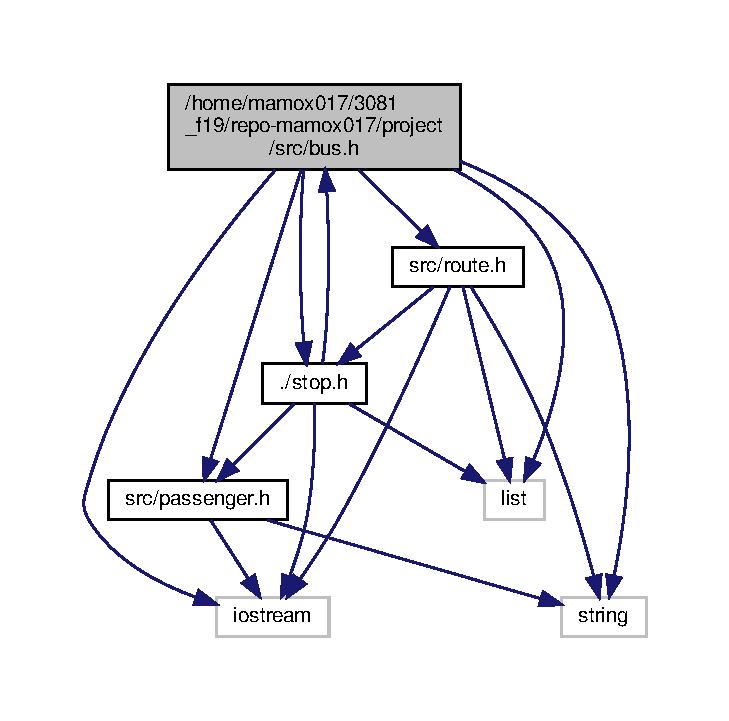
\includegraphics[width=350pt]{bus_8h__incl}
\end{center}
\end{figure}
<<<<<<< HEAD
This graph shows which files directly or indirectly include this file\+:\nopagebreak
=======
This graph shows which files directly or indirectly include this file\+:
\nopagebreak
>>>>>>> master
\begin{figure}[H]
\begin{center}
\leavevmode
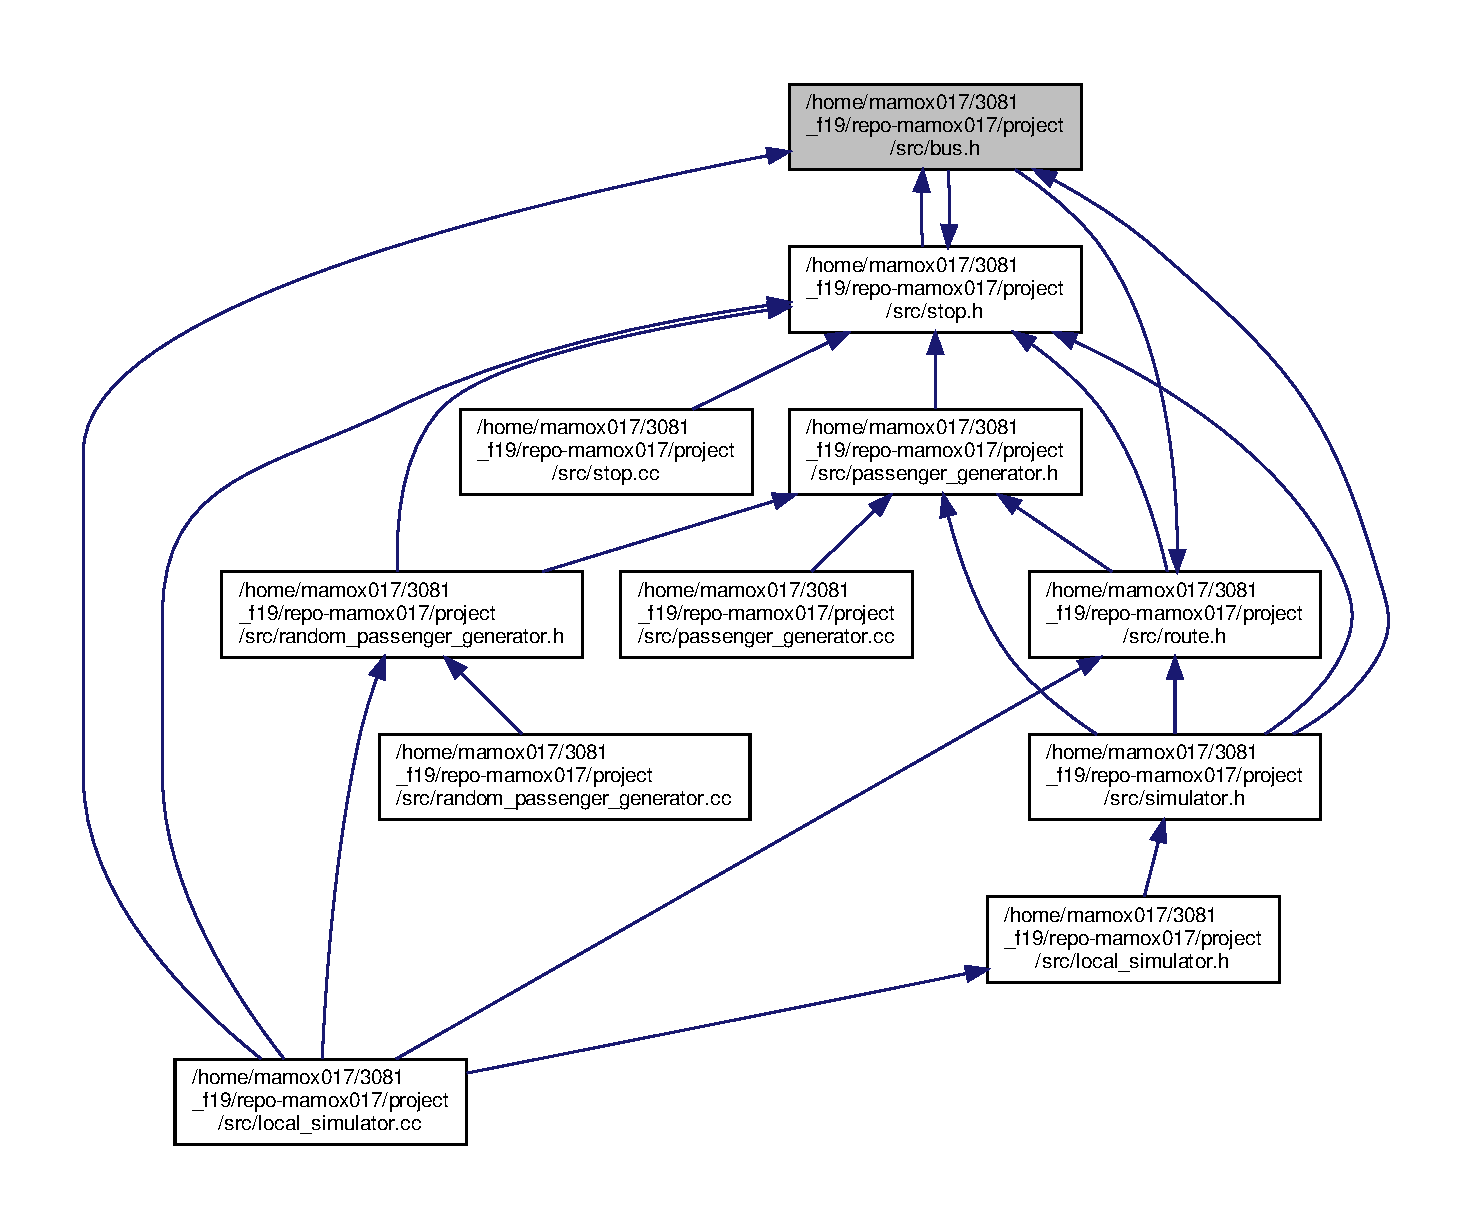
\includegraphics[width=350pt]{bus_8h__dep__incl}
\end{center}
\end{figure}
\subsection*{Classes}
\begin{DoxyCompactItemize}
\item 
class \hyperlink{classBus}{Bus}
<<<<<<< HEAD
\begin{DoxyCompactList}\small\item\em The main class for the bus. \end{DoxyCompactList}\end{DoxyCompactItemize}
=======
\end{DoxyCompactItemize}
>>>>>>> master


\subsection{Detailed Description}
\begin{DoxyCopyright}{Copyright}
2019 3081 Staff, All rights reserved. 
\end{DoxyCopyright}

\hypertarget{local__simulator_8cc}{}\section{/home/mamox017/3081\+\_\+f19/repo-\/mamox017/project/src/local\+\_\+simulator.cc File Reference}
\label{local__simulator_8cc}\index{/home/mamox017/3081\+\_\+f19/repo-\/mamox017/project/src/local\+\_\+simulator.\+cc@{/home/mamox017/3081\+\_\+f19/repo-\/mamox017/project/src/local\+\_\+simulator.\+cc}}
{\ttfamily \#include \char`\"{}local\+\_\+simulator.\+h\char`\"{}}\newline
{\ttfamily \#include $<$vector$>$}\newline
{\ttfamily \#include $<$list$>$}\newline
{\ttfamily \#include \char`\"{}bus.\+h\char`\"{}}\newline
{\ttfamily \#include \char`\"{}stop.\+h\char`\"{}}\newline
{\ttfamily \#include \char`\"{}route.\+h\char`\"{}}\newline
{\ttfamily \#include \char`\"{}random\+\_\+passenger\+\_\+generator.\+h\char`\"{}}\newline
Include dependency graph for local\+\_\+simulator.\+cc\+:
\nopagebreak
\begin{figure}[H]
\begin{center}
\leavevmode
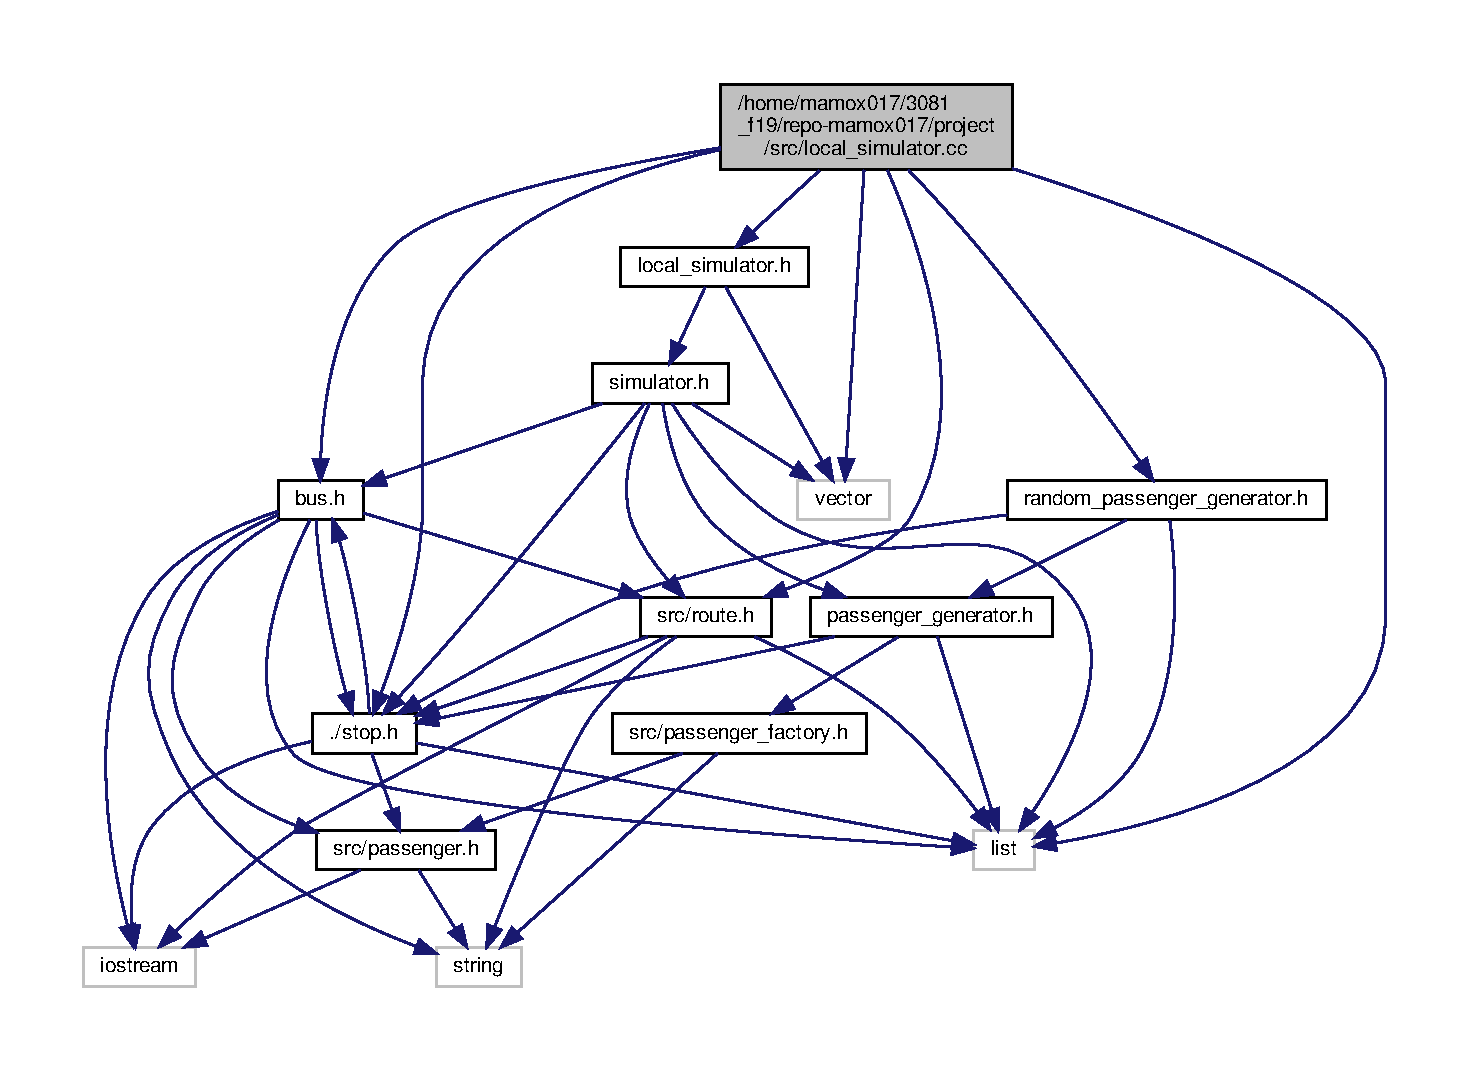
\includegraphics[width=350pt]{local__simulator_8cc__incl}
\end{center}
\end{figure}


\subsection{Detailed Description}
\begin{DoxyCopyright}{Copyright}
2019 3081 Staff, All rights reserved. 
\end{DoxyCopyright}

\hypertarget{local__simulator_8h}{}\section{/home/mamox017/3081\+\_\+f19/repo-\/mamox017/project/src/local\+\_\+simulator.h File Reference}
\label{local__simulator_8h}\index{/home/mamox017/3081\+\_\+f19/repo-\/mamox017/project/src/local\+\_\+simulator.\+h@{/home/mamox017/3081\+\_\+f19/repo-\/mamox017/project/src/local\+\_\+simulator.\+h}}
{\ttfamily \#include $<$vector$>$}\newline
{\ttfamily \#include \char`\"{}src/simulator.\+h\char`\"{}}\newline
Include dependency graph for local\+\_\+simulator.\+h\+:\nopagebreak
\begin{figure}[H]
\begin{center}
\leavevmode
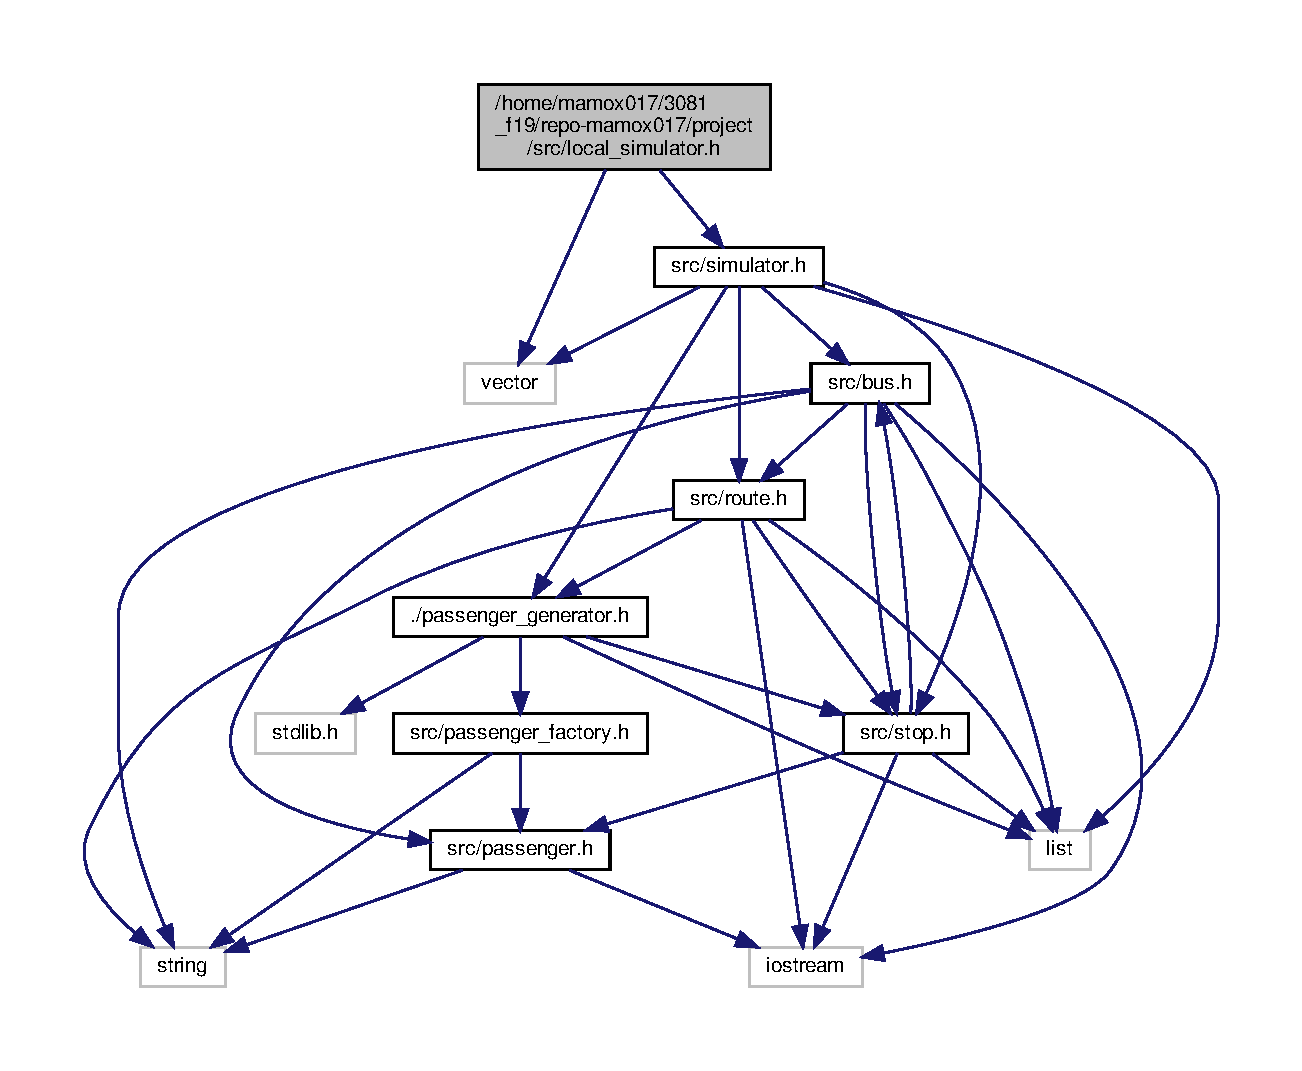
\includegraphics[width=350pt]{local__simulator_8h__incl}
\end{center}
\end{figure}
This graph shows which files directly or indirectly include this file\+:\nopagebreak
\begin{figure}[H]
\begin{center}
\leavevmode
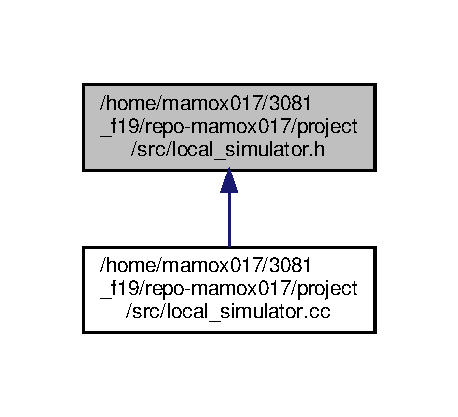
\includegraphics[width=220pt]{local__simulator_8h__dep__incl}
\end{center}
\end{figure}
\subsection*{Classes}
\begin{DoxyCompactItemize}
\item 
class \hyperlink{classLocalSimulator}{Local\+Simulator}
\begin{DoxyCompactList}\small\item\em The main class for a localsimulator. \end{DoxyCompactList}\end{DoxyCompactItemize}


\subsection{Detailed Description}
\begin{DoxyCopyright}{Copyright}
2019 3081 Staff, All rights reserved. 
\end{DoxyCopyright}

\hypertarget{passenger_8h}{}\section{/home/mamox017/3081\+\_\+f19/repo-\/mamox017/project/src/passenger.h File Reference}
\label{passenger_8h}\index{/home/mamox017/3081\+\_\+f19/repo-\/mamox017/project/src/passenger.\+h@{/home/mamox017/3081\+\_\+f19/repo-\/mamox017/project/src/passenger.\+h}}
{\ttfamily \#include $<$iostream$>$}\newline
{\ttfamily \#include $<$string$>$}\newline
Include dependency graph for passenger.\+h\+:
\nopagebreak
\begin{figure}[H]
\begin{center}
\leavevmode
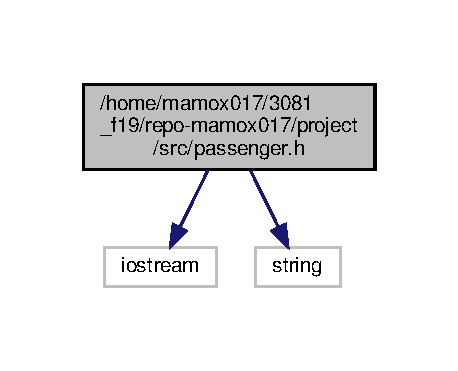
\includegraphics[width=220pt]{passenger_8h__incl}
\end{center}
\end{figure}
This graph shows which files directly or indirectly include this file\+:
\nopagebreak
\begin{figure}[H]
\begin{center}
\leavevmode
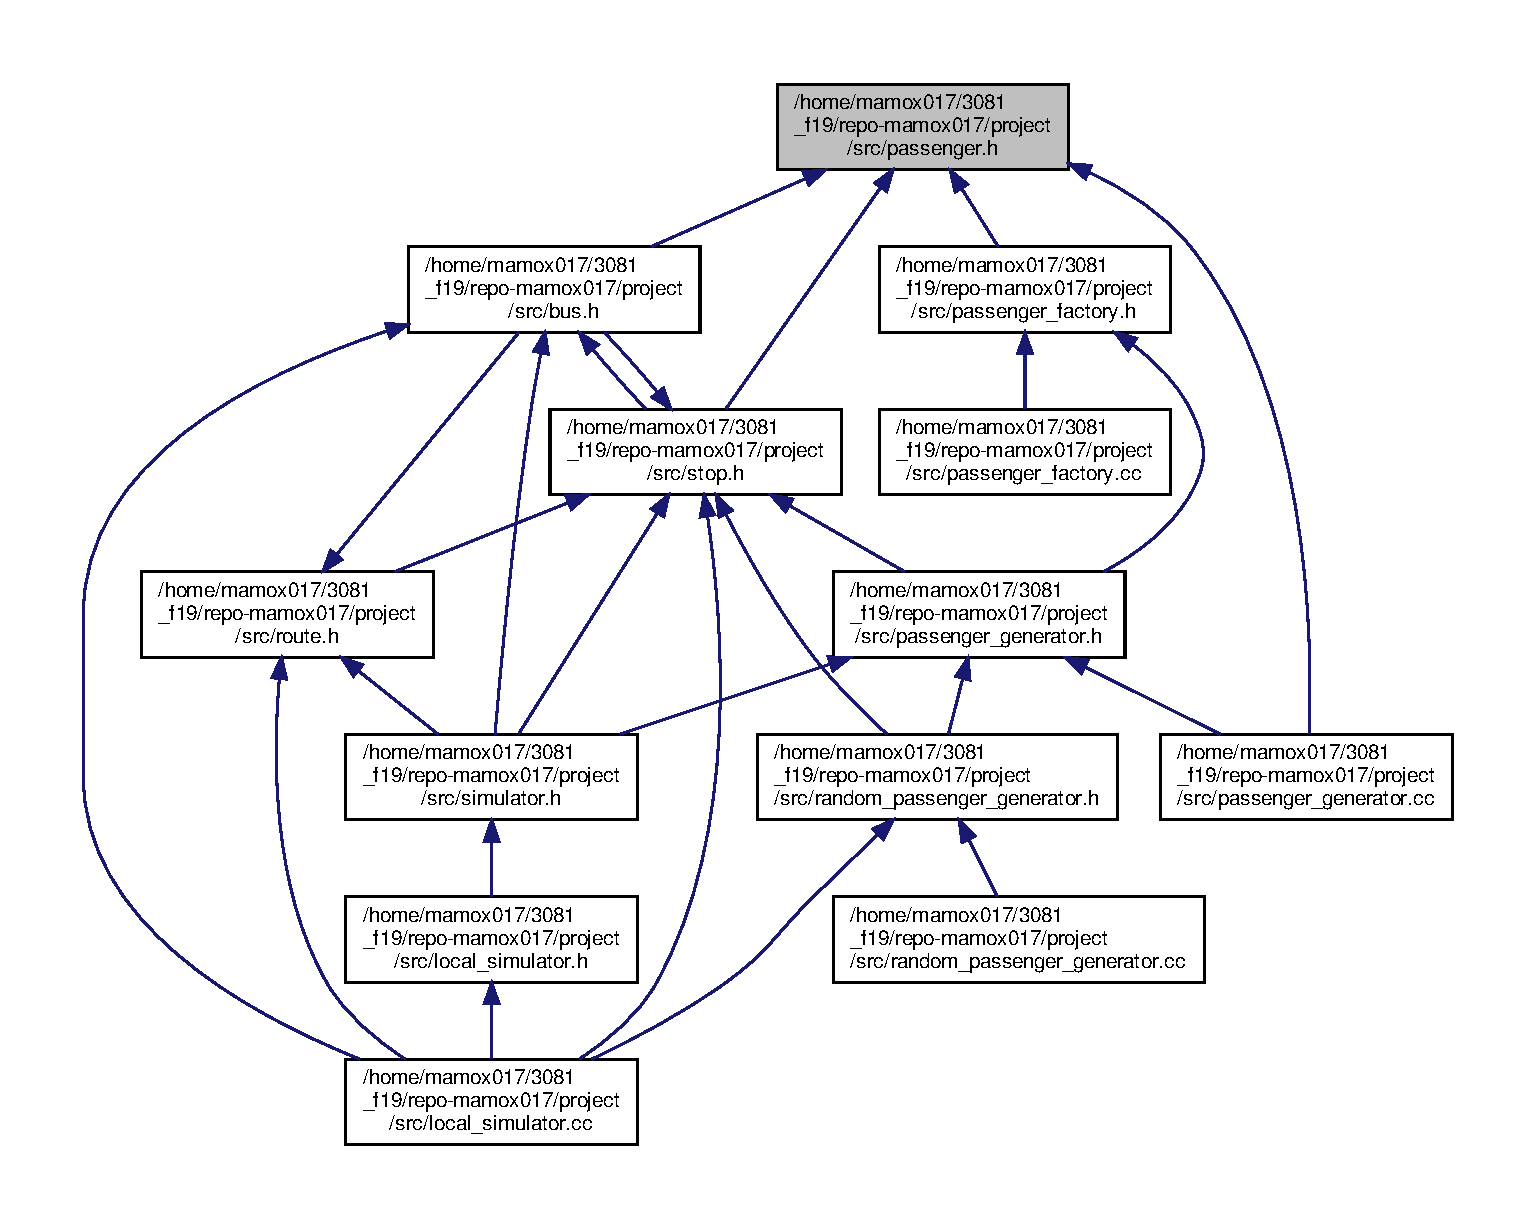
\includegraphics[width=350pt]{passenger_8h__dep__incl}
\end{center}
\end{figure}
\subsection*{Classes}
\begin{DoxyCompactItemize}
\item 
class \hyperlink{classPassenger}{Passenger}
\end{DoxyCompactItemize}


\subsection{Detailed Description}
\begin{DoxyCopyright}{Copyright}
2019 3081 Staff, All rights reserved. 
\end{DoxyCopyright}

\hypertarget{passenger__factory_8cc}{}\section{/home/mamox017/3081\+\_\+f19/repo-\/mamox017/project/src/passenger\+\_\+factory.cc File Reference}
\label{passenger__factory_8cc}\index{/home/mamox017/3081\+\_\+f19/repo-\/mamox017/project/src/passenger\+\_\+factory.\+cc@{/home/mamox017/3081\+\_\+f19/repo-\/mamox017/project/src/passenger\+\_\+factory.\+cc}}
{\ttfamily \#include $<$random$>$}\newline
{\ttfamily \#include $<$string$>$}\newline
{\ttfamily \#include \char`\"{}src/passenger\+\_\+factory.\+h\char`\"{}}\newline
Include dependency graph for passenger\+\_\+factory.\+cc\+:\nopagebreak
\begin{figure}[H]
\begin{center}
\leavevmode
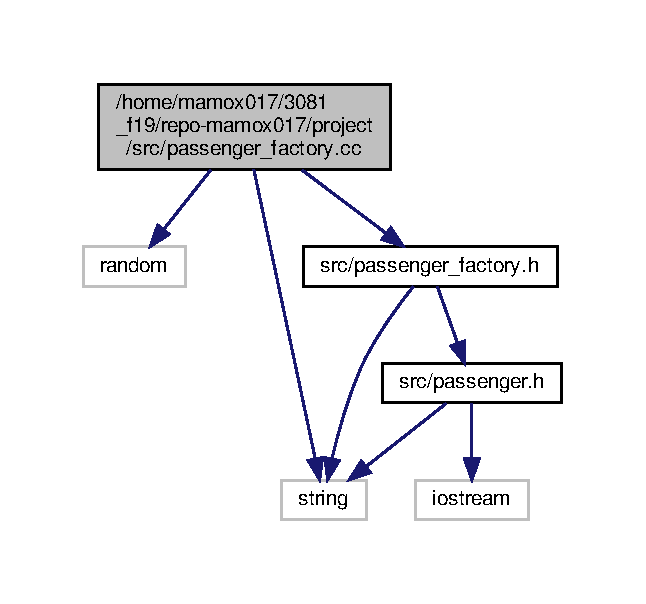
\includegraphics[width=310pt]{passenger__factory_8cc__incl}
\end{center}
\end{figure}
\subsection*{Functions}
\begin{DoxyCompactItemize}
\item 
\mbox{\Hypertarget{passenger__factory_8cc_af34adcff7354e7e8d172f7a97bc05d68}\label{passenger__factory_8cc_af34adcff7354e7e8d172f7a97bc05d68}} 
std\+::mt19937 {\bfseries e} (dev())
\item 
\mbox{\Hypertarget{passenger__factory_8cc_a1d818b31bbf5715a76ee321d8a0993e0}\label{passenger__factory_8cc_a1d818b31bbf5715a76ee321d8a0993e0}} 
std\+::uniform\+\_\+int\+\_\+distribution$<$ std\+::mt19937\+::result\+\_\+type $>$ {\bfseries dist} (1, 1000)
\end{DoxyCompactItemize}
\subsection*{Variables}
\begin{DoxyCompactItemize}
\item 
\mbox{\Hypertarget{passenger__factory_8cc_ad768868c172722a84c70801c1382438f}\label{passenger__factory_8cc_ad768868c172722a84c70801c1382438f}} 
std\+::random\+\_\+device {\bfseries dev}
\end{DoxyCompactItemize}


\subsection{Detailed Description}
\begin{DoxyCopyright}{Copyright}
2019 3081 Staff, All rights reserved. 
\end{DoxyCopyright}

\hypertarget{passenger__factory_8h}{}\section{/home/mamox017/3081\+\_\+f19/repo-\/mamox017/labs/lab08\+\_\+style\+\_\+doxy/src/passenger\+\_\+factory.h File Reference}
\label{passenger__factory_8h}\index{/home/mamox017/3081\+\_\+f19/repo-\/mamox017/labs/lab08\+\_\+style\+\_\+doxy/src/passenger\+\_\+factory.\+h@{/home/mamox017/3081\+\_\+f19/repo-\/mamox017/labs/lab08\+\_\+style\+\_\+doxy/src/passenger\+\_\+factory.\+h}}
{\ttfamily \#include $<$string$>$}\newline
{\ttfamily \#include \char`\"{}src/passenger.\+h\char`\"{}}\newline
Include dependency graph for passenger\+\_\+factory.\+h\+:\nopagebreak
\begin{figure}[H]
\begin{center}
\leavevmode
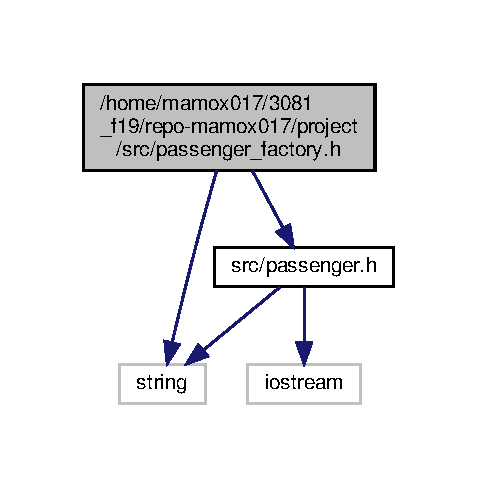
\includegraphics[width=240pt]{passenger__factory_8h__incl}
\end{center}
\end{figure}
This graph shows which files directly or indirectly include this file\+:\nopagebreak
\begin{figure}[H]
\begin{center}
\leavevmode
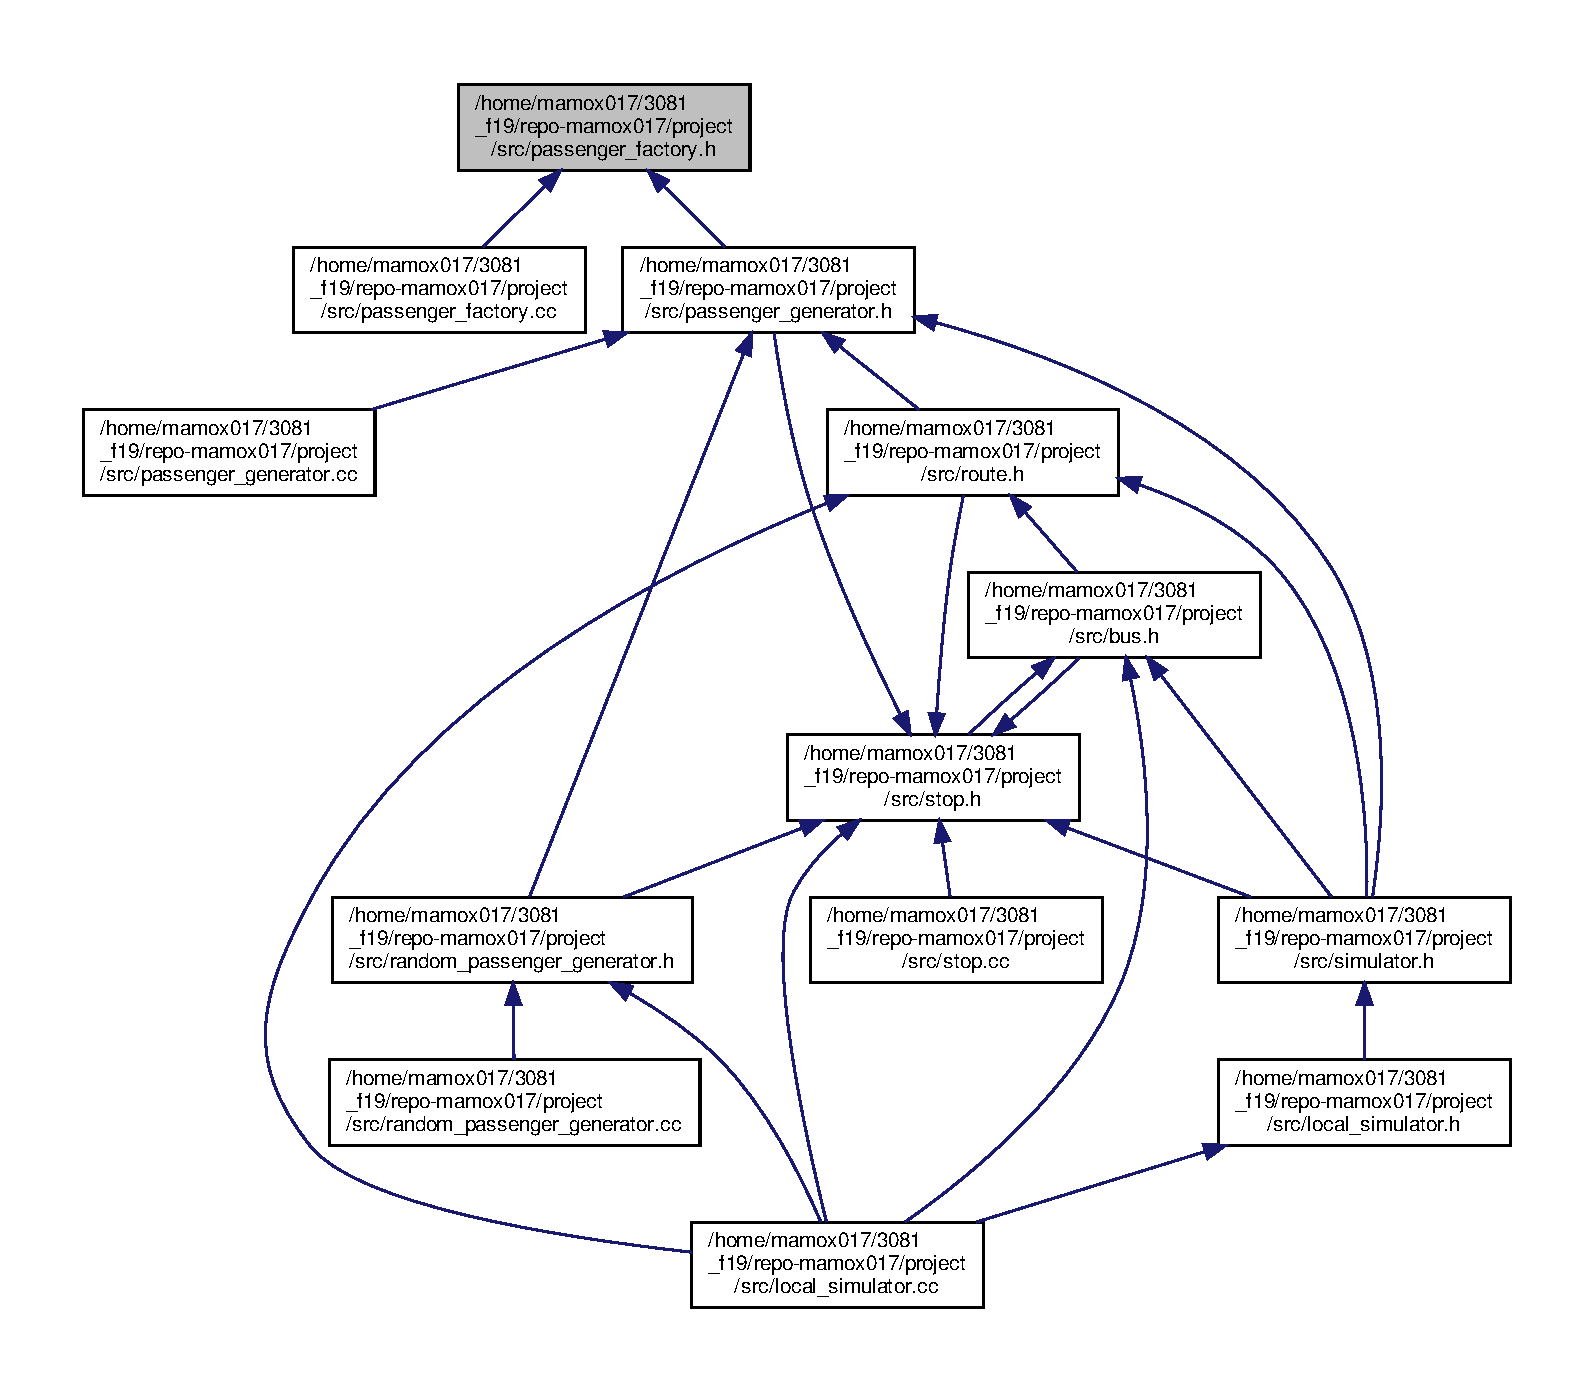
\includegraphics[width=240pt]{passenger__factory_8h__dep__incl}
\end{center}
\end{figure}
\subsection*{Classes}
\begin{DoxyCompactItemize}
\item 
class \hyperlink{classPassengerFactory}{Passenger\+Factory}
\begin{DoxyCompactList}\small\item\em The main class for the generation of passengers. \end{DoxyCompactList}\end{DoxyCompactItemize}


\subsection{Detailed Description}
\begin{DoxyCopyright}{Copyright}
2019 3081 Staff, All rights reserved. 
\end{DoxyCopyright}

\hypertarget{passenger__generator_8cc}{}\section{/home/mamox017/3081\+\_\+f19/repo-\/mamox017/project/src/passenger\+\_\+generator.cc File Reference}
\label{passenger__generator_8cc}\index{/home/mamox017/3081\+\_\+f19/repo-\/mamox017/project/src/passenger\+\_\+generator.\+cc@{/home/mamox017/3081\+\_\+f19/repo-\/mamox017/project/src/passenger\+\_\+generator.\+cc}}
{\ttfamily \#include \char`\"{}src/passenger\+\_\+generator.\+h\char`\"{}}\newline
{\ttfamily \#include $<$stdlib.\+h$>$}\newline
{\ttfamily \#include \char`\"{}src/passenger.\+h\char`\"{}}\newline
Include dependency graph for passenger\+\_\+generator.\+cc\+:\nopagebreak
\begin{figure}[H]
\begin{center}
\leavevmode
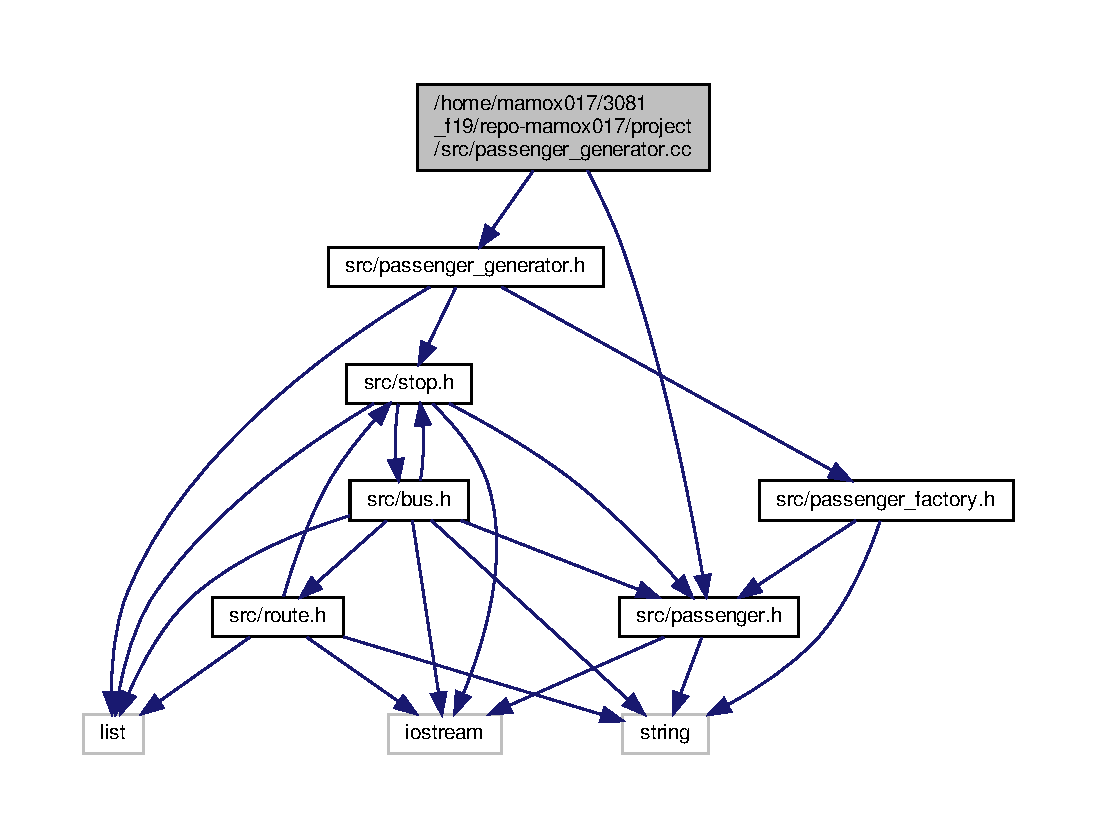
\includegraphics[width=350pt]{passenger__generator_8cc__incl}
\end{center}
\end{figure}


\subsection{Detailed Description}
\begin{DoxyCopyright}{Copyright}
2019 3081 Staff, All rights reserved. 
\end{DoxyCopyright}

\hypertarget{passenger__generator_8h}{}\section{/home/mamox017/3081\+\_\+f19/repo-\/mamox017/project/src/passenger\+\_\+generator.h File Reference}
\label{passenger__generator_8h}\index{/home/mamox017/3081\+\_\+f19/repo-\/mamox017/project/src/passenger\+\_\+generator.\+h@{/home/mamox017/3081\+\_\+f19/repo-\/mamox017/project/src/passenger\+\_\+generator.\+h}}
{\ttfamily \#include $<$list$>$}\newline
{\ttfamily \#include \char`\"{}src/passenger\+\_\+factory.\+h\char`\"{}}\newline
{\ttfamily \#include \char`\"{}src/stop.\+h\char`\"{}}\newline
Include dependency graph for passenger\+\_\+generator.\+h\+:
\nopagebreak
\begin{figure}[H]
\begin{center}
\leavevmode
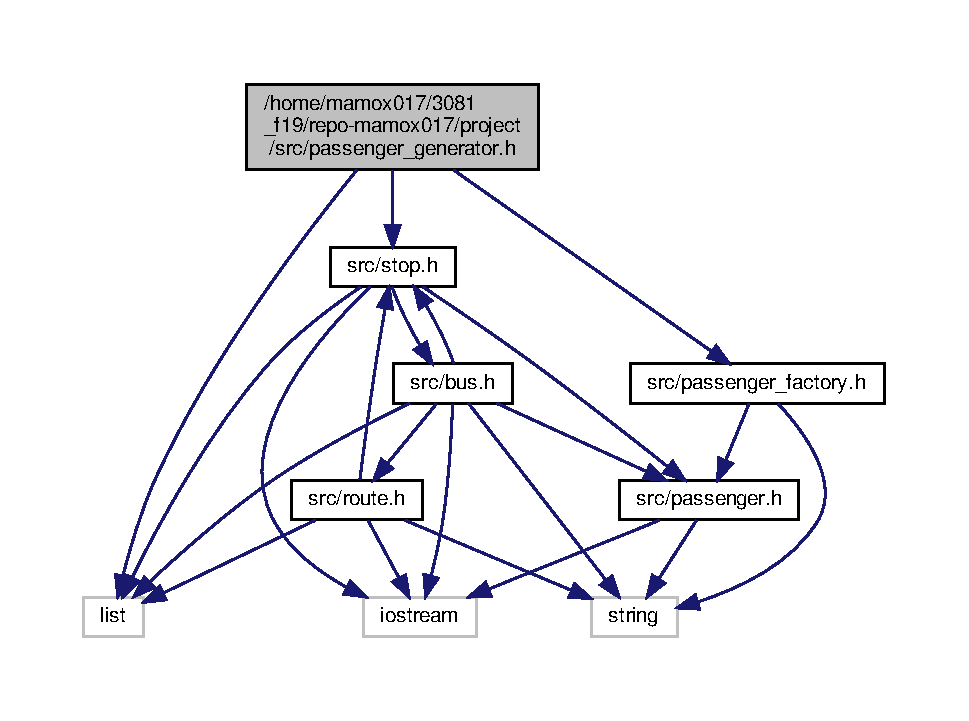
\includegraphics[width=350pt]{passenger__generator_8h__incl}
\end{center}
\end{figure}
This graph shows which files directly or indirectly include this file\+:
\nopagebreak
\begin{figure}[H]
\begin{center}
\leavevmode
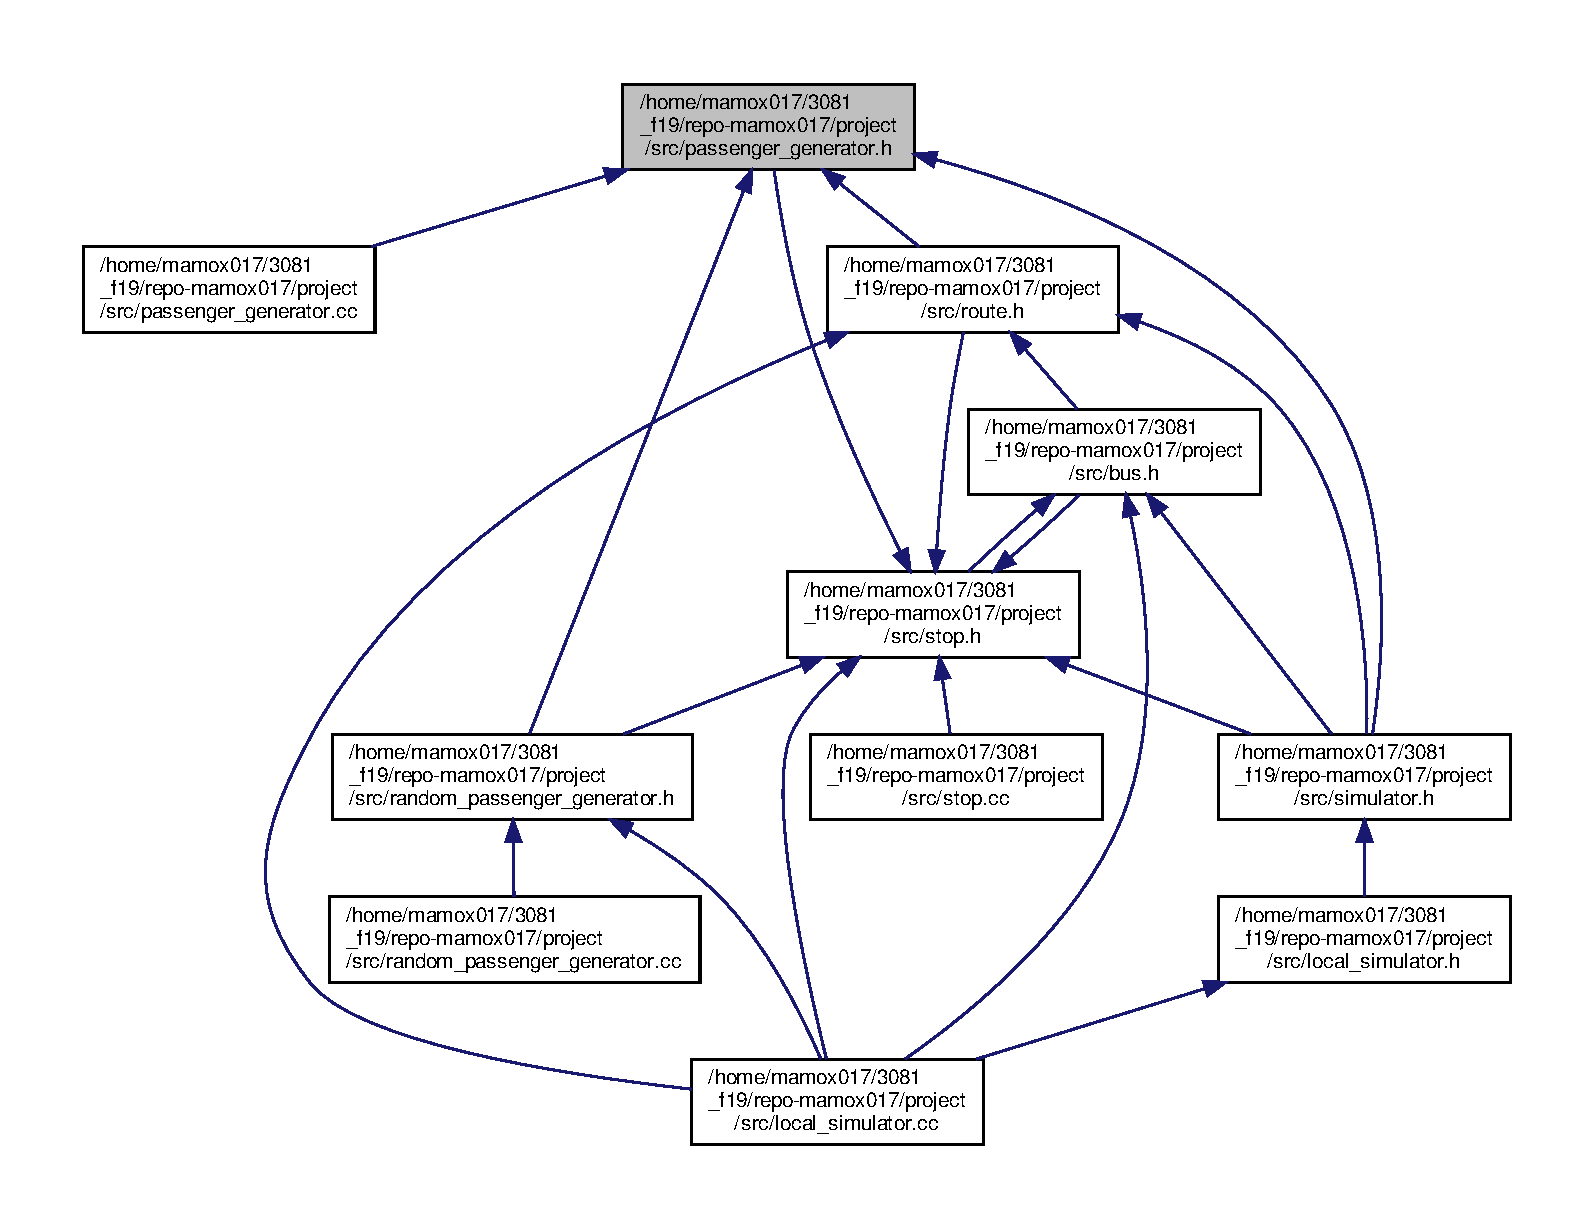
\includegraphics[width=350pt]{passenger__generator_8h__dep__incl}
\end{center}
\end{figure}
\subsection*{Classes}
\begin{DoxyCompactItemize}
\item 
class \hyperlink{classPassengerGenerator}{Passenger\+Generator}
\end{DoxyCompactItemize}


\subsection{Detailed Description}
\begin{DoxyCopyright}{Copyright}
2019 3081 Staff, All rights reserved. 
\end{DoxyCopyright}

\hypertarget{random__passenger__generator_8cc}{}\section{/home/mamox017/3081\+\_\+f19/repo-\/mamox017/project/src/random\+\_\+passenger\+\_\+generator.cc File Reference}
\label{random__passenger__generator_8cc}\index{/home/mamox017/3081\+\_\+f19/repo-\/mamox017/project/src/random\+\_\+passenger\+\_\+generator.\+cc@{/home/mamox017/3081\+\_\+f19/repo-\/mamox017/project/src/random\+\_\+passenger\+\_\+generator.\+cc}}
<<<<<<< HEAD
{\ttfamily \#include $<$random$>$}\newline
{\ttfamily \#include $<$ctime$>$}\newline
{\ttfamily \#include \char`\"{}src/random\+\_\+passenger\+\_\+generator.\+h\char`\"{}}\newline
Include dependency graph for random\+\_\+passenger\+\_\+generator.\+cc\+:\nopagebreak
=======
{\ttfamily \#include \char`\"{}src/random\+\_\+passenger\+\_\+generator.\+h\char`\"{}}\newline
Include dependency graph for random\+\_\+passenger\+\_\+generator.\+cc\+:
\nopagebreak
>>>>>>> master
\begin{figure}[H]
\begin{center}
\leavevmode
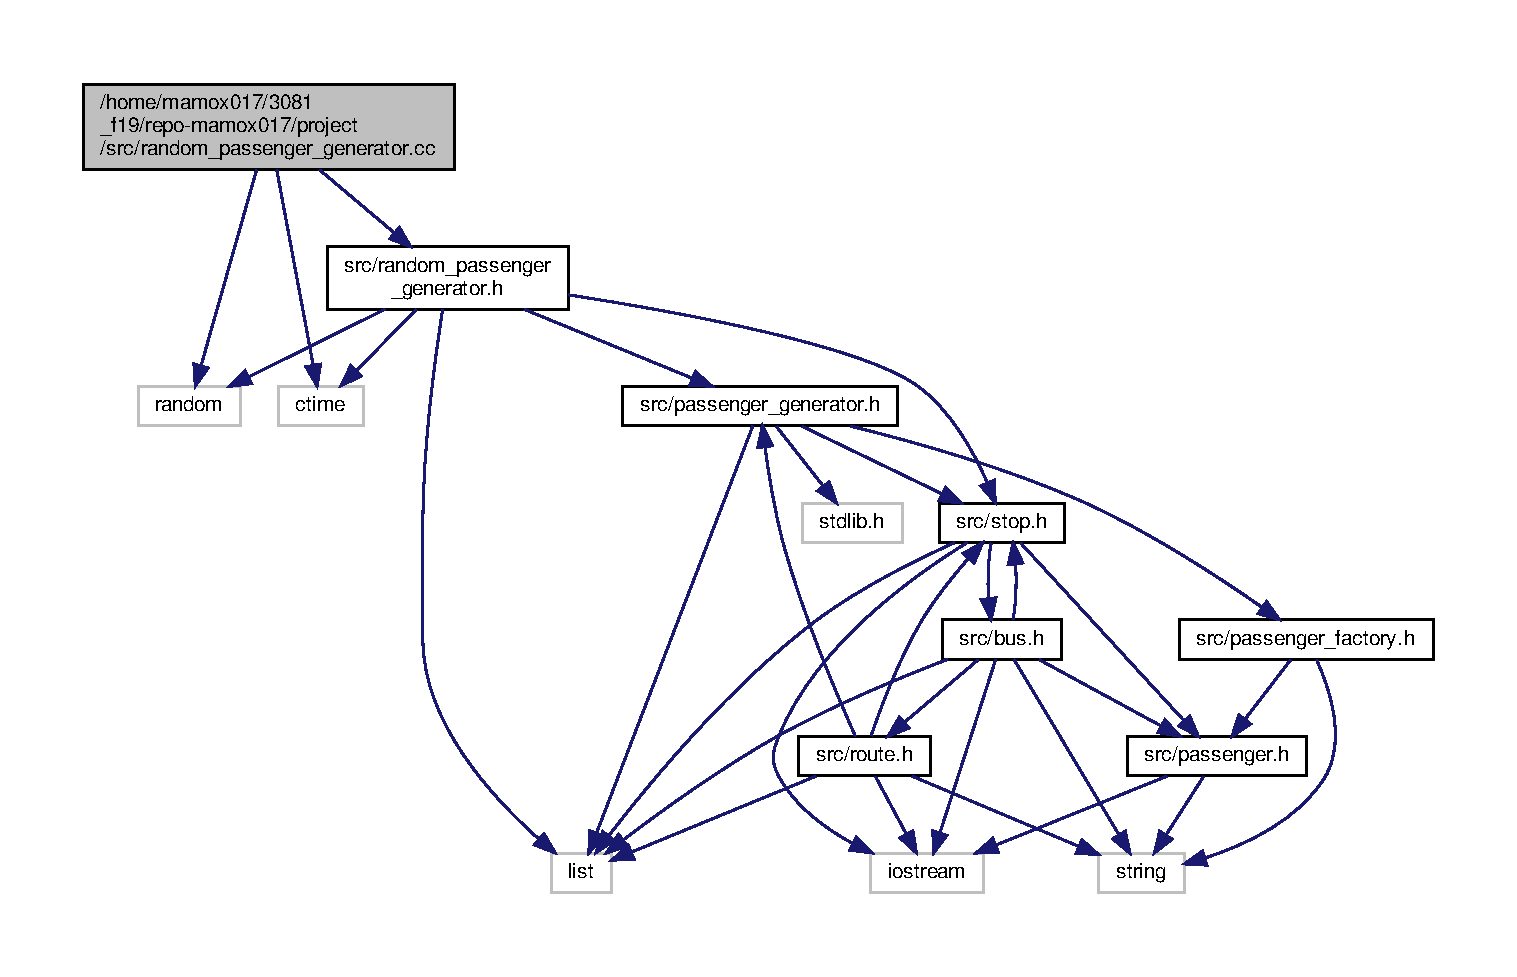
\includegraphics[width=350pt]{random__passenger__generator_8cc__incl}
\end{center}
\end{figure}


\subsection{Detailed Description}
\begin{DoxyCopyright}{Copyright}
2019 3081 Staff, All rights reserved. 
\end{DoxyCopyright}

\hypertarget{random__passenger__generator_8h}{}\section{/home/mamox017/3081\+\_\+f19/repo-\/mamox017/project/src/random\+\_\+passenger\+\_\+generator.h File Reference}
\label{random__passenger__generator_8h}\index{/home/mamox017/3081\+\_\+f19/repo-\/mamox017/project/src/random\+\_\+passenger\+\_\+generator.\+h@{/home/mamox017/3081\+\_\+f19/repo-\/mamox017/project/src/random\+\_\+passenger\+\_\+generator.\+h}}
{\ttfamily \#include $<$list$>$}\newline
<<<<<<< HEAD
{\ttfamily \#include $<$random$>$}\newline
{\ttfamily \#include $<$ctime$>$}\newline
{\ttfamily \#include \char`\"{}src/passenger\+\_\+generator.\+h\char`\"{}}\newline
{\ttfamily \#include \char`\"{}src/stop.\+h\char`\"{}}\newline
Include dependency graph for random\+\_\+passenger\+\_\+generator.\+h\+:\nopagebreak
=======
{\ttfamily \#include \char`\"{}src/passenger\+\_\+generator.\+h\char`\"{}}\newline
{\ttfamily \#include \char`\"{}src/stop.\+h\char`\"{}}\newline
Include dependency graph for random\+\_\+passenger\+\_\+generator.\+h\+:
\nopagebreak
>>>>>>> master
\begin{figure}[H]
\begin{center}
\leavevmode
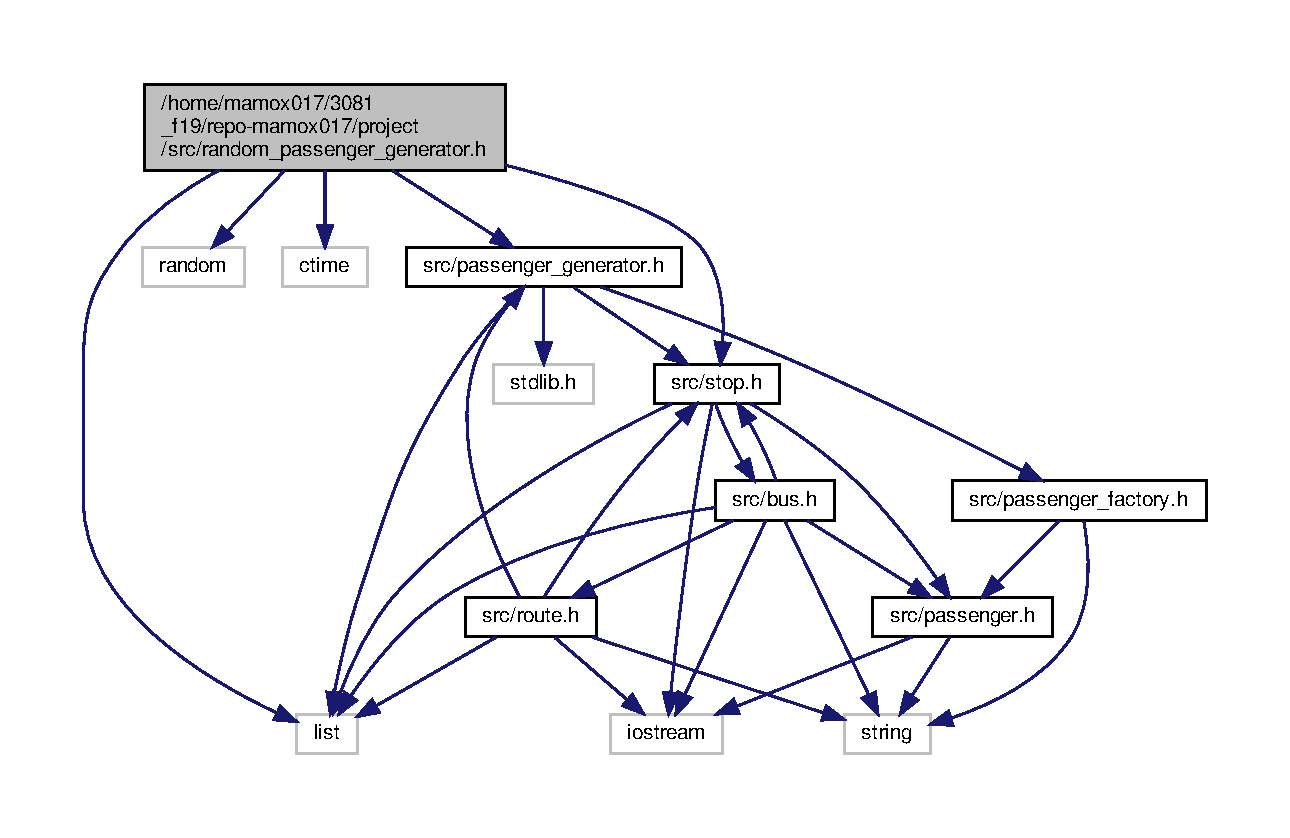
\includegraphics[width=350pt]{random__passenger__generator_8h__incl}
\end{center}
\end{figure}
<<<<<<< HEAD
This graph shows which files directly or indirectly include this file\+:\nopagebreak
=======
This graph shows which files directly or indirectly include this file\+:
\nopagebreak
>>>>>>> master
\begin{figure}[H]
\begin{center}
\leavevmode
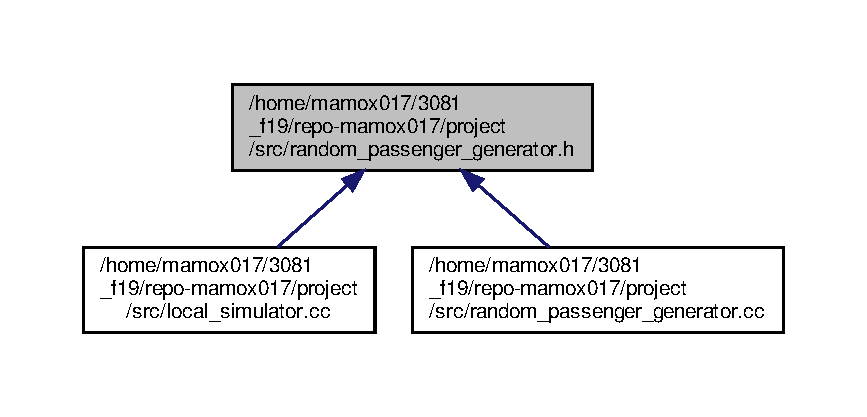
\includegraphics[width=350pt]{random__passenger__generator_8h__dep__incl}
\end{center}
\end{figure}
\subsection*{Classes}
\begin{DoxyCompactItemize}
\item 
class \hyperlink{classRandomPassengerGenerator}{Random\+Passenger\+Generator}
<<<<<<< HEAD
\begin{DoxyCompactList}\small\item\em The main class for the random passenger generator. \end{DoxyCompactList}\end{DoxyCompactItemize}
=======
\end{DoxyCompactItemize}
>>>>>>> master


\subsection{Detailed Description}
\begin{DoxyCopyright}{Copyright}
2019 3081 Staff, All rights reserved. 
\end{DoxyCopyright}

\hypertarget{route_8h}{}\section{/home/mamox017/3081\+\_\+f19/repo-\/mamox017/project/src/route.h File Reference}
\label{route_8h}\index{/home/mamox017/3081\+\_\+f19/repo-\/mamox017/project/src/route.\+h@{/home/mamox017/3081\+\_\+f19/repo-\/mamox017/project/src/route.\+h}}
{\ttfamily \#include $<$list$>$}\newline
{\ttfamily \#include $<$iostream$>$}\newline
{\ttfamily \#include $<$string$>$}\newline
{\ttfamily \#include \char`\"{}./stop.\+h\char`\"{}}\newline
Include dependency graph for route.\+h\+:
\nopagebreak
\begin{figure}[H]
\begin{center}
\leavevmode
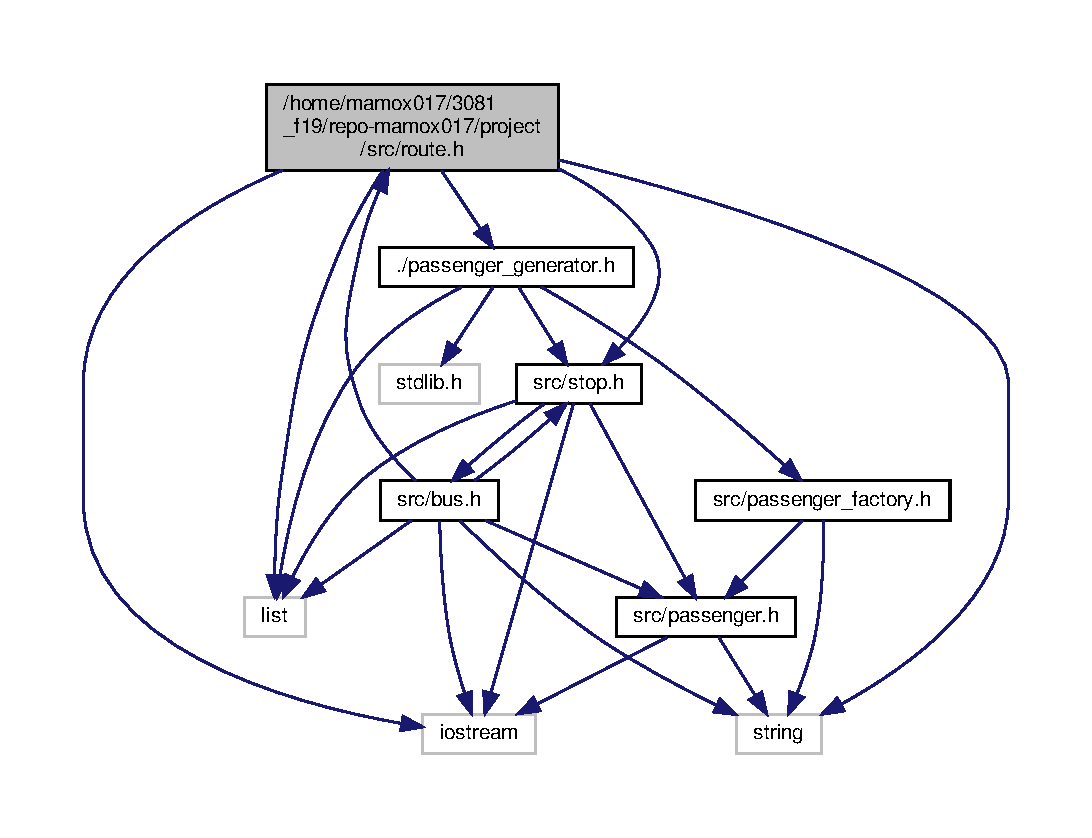
\includegraphics[width=336pt]{route_8h__incl}
\end{center}
\end{figure}
This graph shows which files directly or indirectly include this file\+:
\nopagebreak
\begin{figure}[H]
\begin{center}
\leavevmode
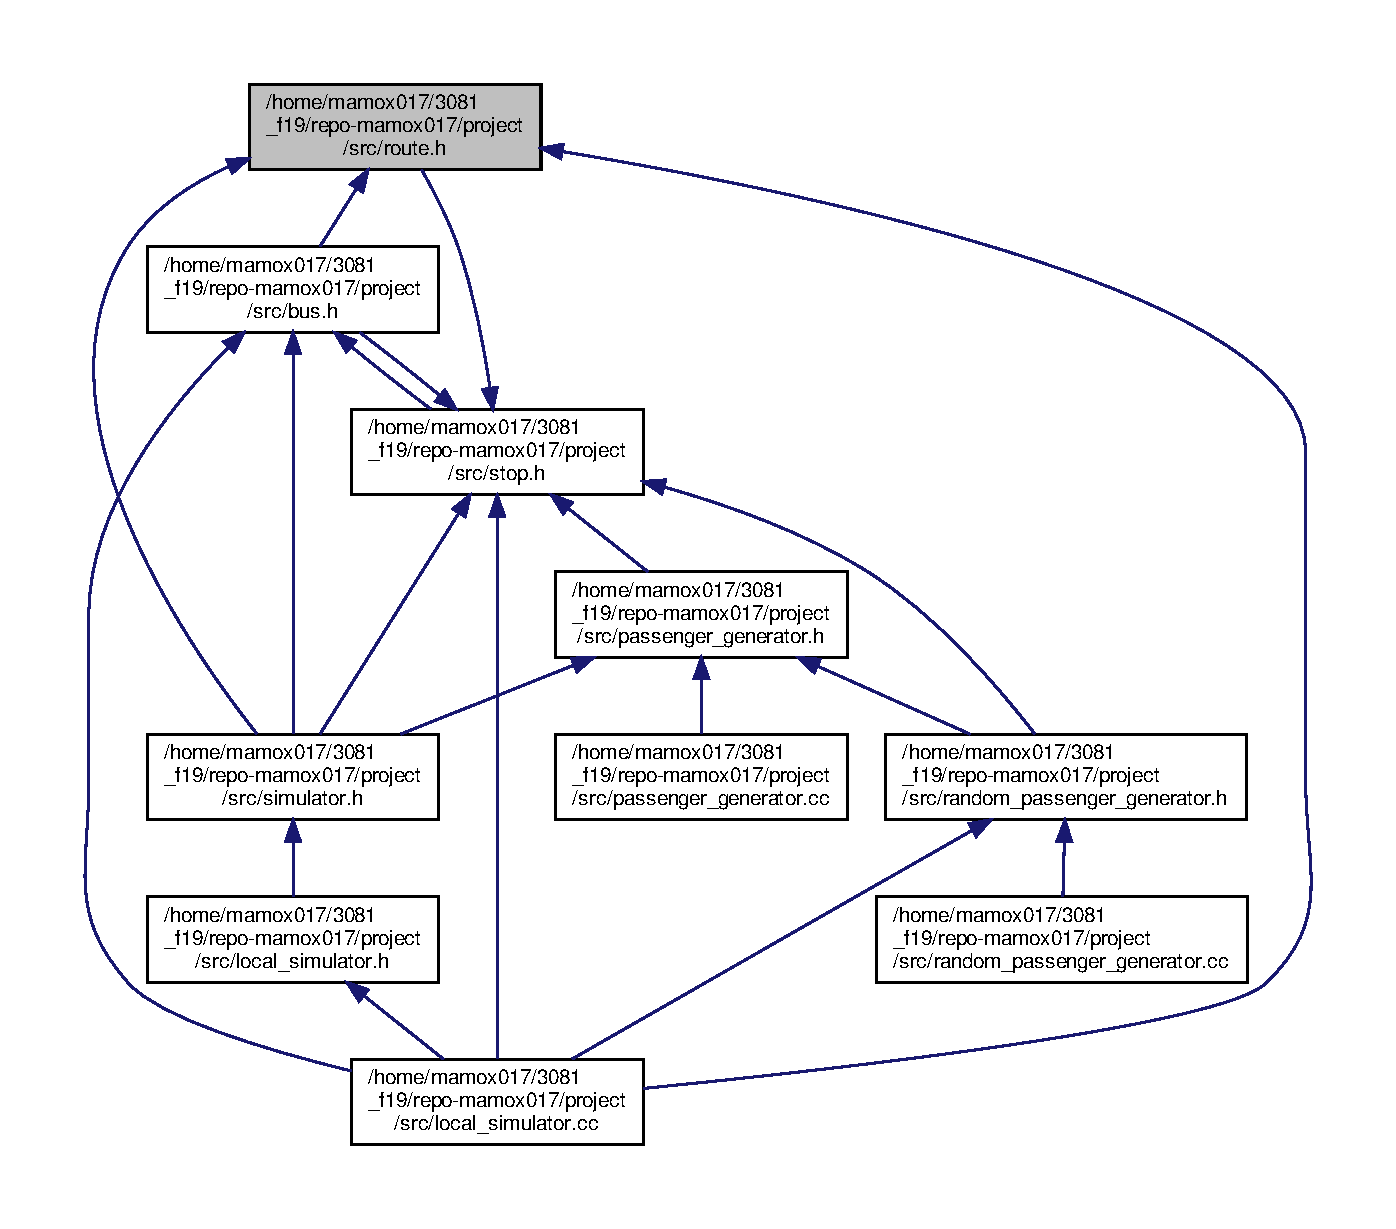
\includegraphics[width=350pt]{route_8h__dep__incl}
\end{center}
\end{figure}
\subsection*{Classes}
\begin{DoxyCompactItemize}
\item 
class \hyperlink{classRoute}{Route}
\end{DoxyCompactItemize}


\subsection{Detailed Description}
2019 3081 Staff, All rights reserved. 
\hypertarget{simulator_8h}{}\section{/home/mamox017/3081\+\_\+f19/repo-\/mamox017/project/src/simulator.h File Reference}
\label{simulator_8h}\index{/home/mamox017/3081\+\_\+f19/repo-\/mamox017/project/src/simulator.\+h@{/home/mamox017/3081\+\_\+f19/repo-\/mamox017/project/src/simulator.\+h}}
{\ttfamily \#include $<$list$>$}\newline
{\ttfamily \#include $<$vector$>$}\newline
{\ttfamily \#include \char`\"{}bus.\+h\char`\"{}}\newline
{\ttfamily \#include \char`\"{}stop.\+h\char`\"{}}\newline
{\ttfamily \#include \char`\"{}route.\+h\char`\"{}}\newline
{\ttfamily \#include \char`\"{}passenger\+\_\+generator.\+h\char`\"{}}\newline
Include dependency graph for simulator.\+h\+:
\nopagebreak
\begin{figure}[H]
\begin{center}
\leavevmode
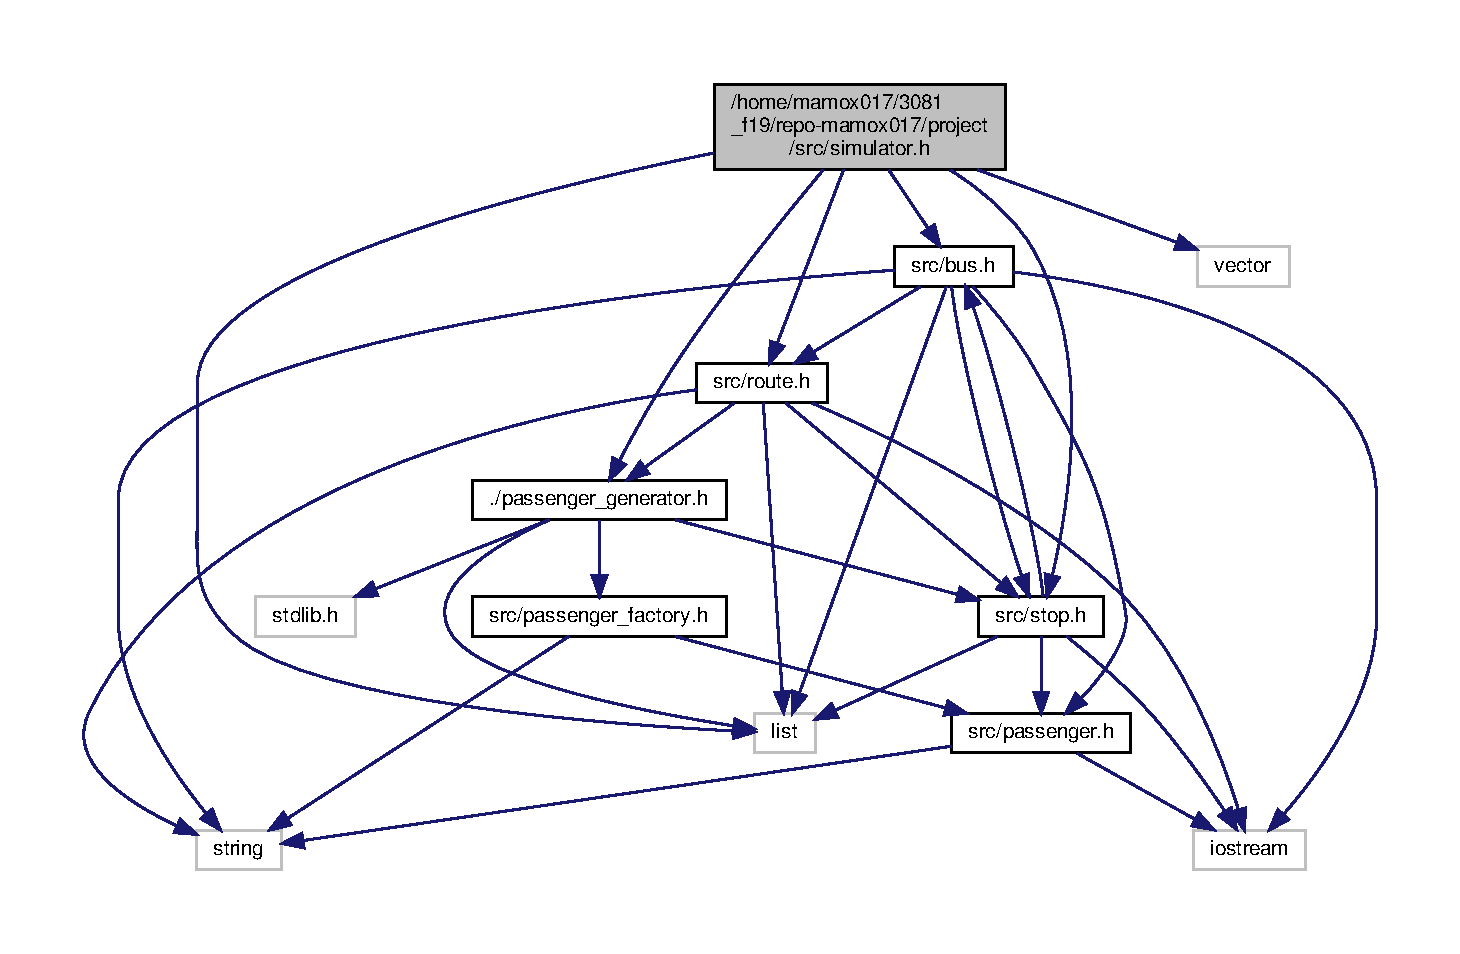
\includegraphics[width=350pt]{simulator_8h__incl}
\end{center}
\end{figure}
This graph shows which files directly or indirectly include this file\+:
\nopagebreak
\begin{figure}[H]
\begin{center}
\leavevmode
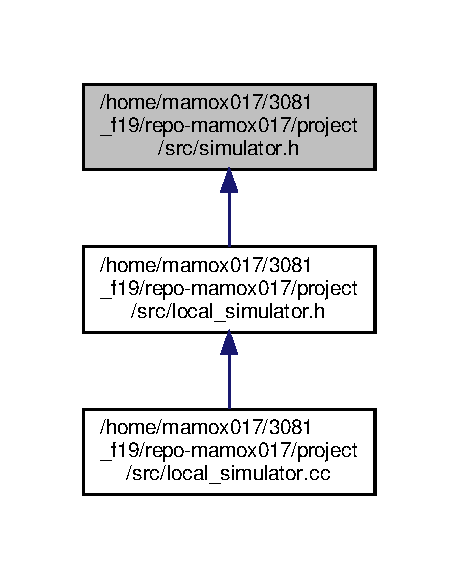
\includegraphics[width=220pt]{simulator_8h__dep__incl}
\end{center}
\end{figure}
\subsection*{Classes}
\begin{DoxyCompactItemize}
\item 
class \hyperlink{classSimulator}{Simulator}
\end{DoxyCompactItemize}


\subsection{Detailed Description}
\begin{DoxyCopyright}{Copyright}
2019 3081 Staff, All rights reserved. 
\end{DoxyCopyright}

\hypertarget{stop_8cc}{}\section{/home/mamox017/3081\+\_\+f19/repo-\/mamox017/project/src/stop.cc File Reference}
\label{stop_8cc}\index{/home/mamox017/3081\+\_\+f19/repo-\/mamox017/project/src/stop.\+cc@{/home/mamox017/3081\+\_\+f19/repo-\/mamox017/project/src/stop.\+cc}}
{\ttfamily \#include $<$iostream$>$}\newline
{\ttfamily \#include $<$vector$>$}\newline
{\ttfamily \#include \char`\"{}src/stop.\+h\char`\"{}}\newline
Include dependency graph for stop.\+cc\+:\nopagebreak
\begin{figure}[H]
\begin{center}
\leavevmode
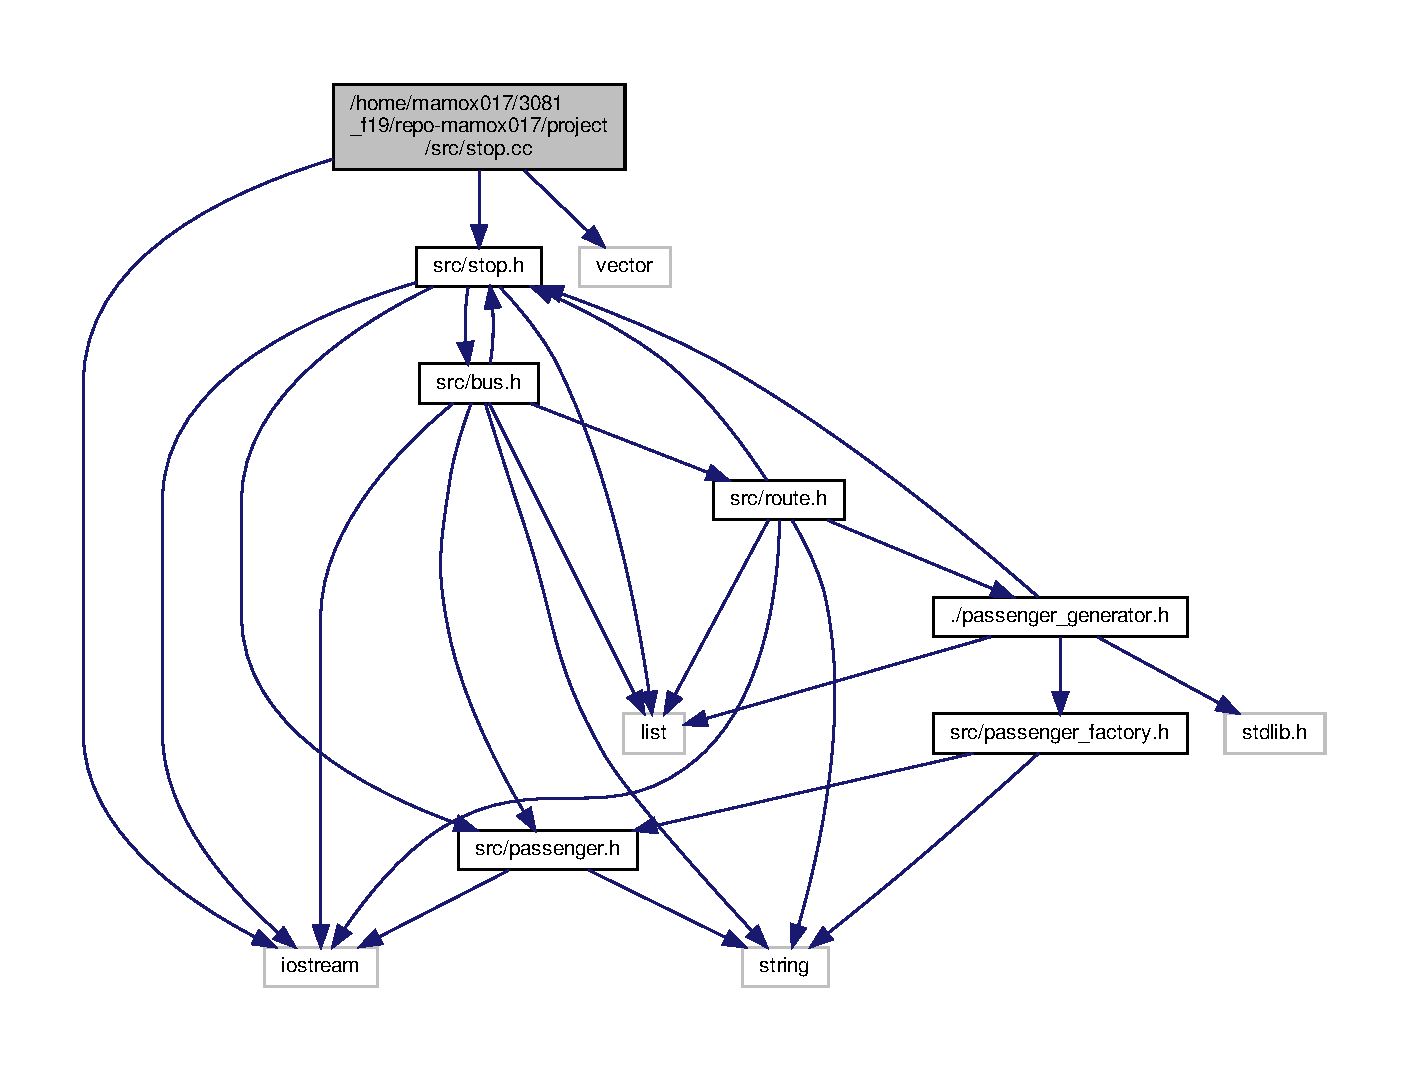
\includegraphics[width=350pt]{stop_8cc__incl}
\end{center}
\end{figure}


\subsection{Detailed Description}
\begin{DoxyCopyright}{Copyright}
2019 3081 Staff, All rights reserved. 
\end{DoxyCopyright}

\hypertarget{stop_8h}{}\section{/home/mamox017/3081\+\_\+f19/repo-\/mamox017/project/src/stop.h File Reference}
\label{stop_8h}\index{/home/mamox017/3081\+\_\+f19/repo-\/mamox017/project/src/stop.\+h@{/home/mamox017/3081\+\_\+f19/repo-\/mamox017/project/src/stop.\+h}}
{\ttfamily \#include $<$list$>$}\newline
{\ttfamily \#include $<$iostream$>$}\newline
{\ttfamily \#include \char`\"{}src/bus.\+h\char`\"{}}\newline
{\ttfamily \#include \char`\"{}src/passenger.\+h\char`\"{}}\newline
Include dependency graph for stop.\+h\+:
\nopagebreak
\begin{figure}[H]
\begin{center}
\leavevmode
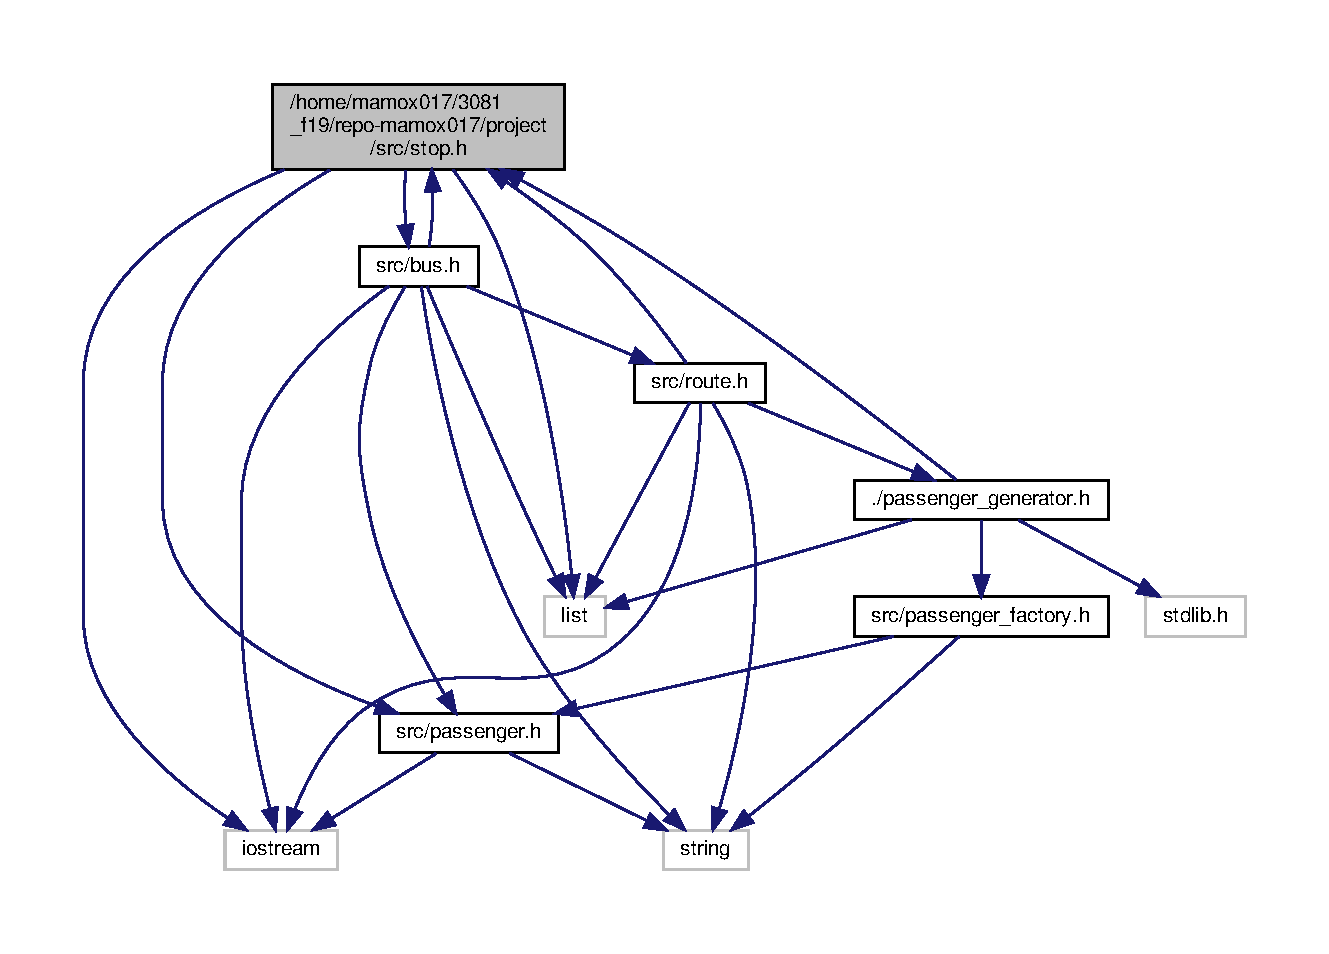
\includegraphics[width=350pt]{stop_8h__incl}
\end{center}
\end{figure}
This graph shows which files directly or indirectly include this file\+:
\nopagebreak
\begin{figure}[H]
\begin{center}
\leavevmode
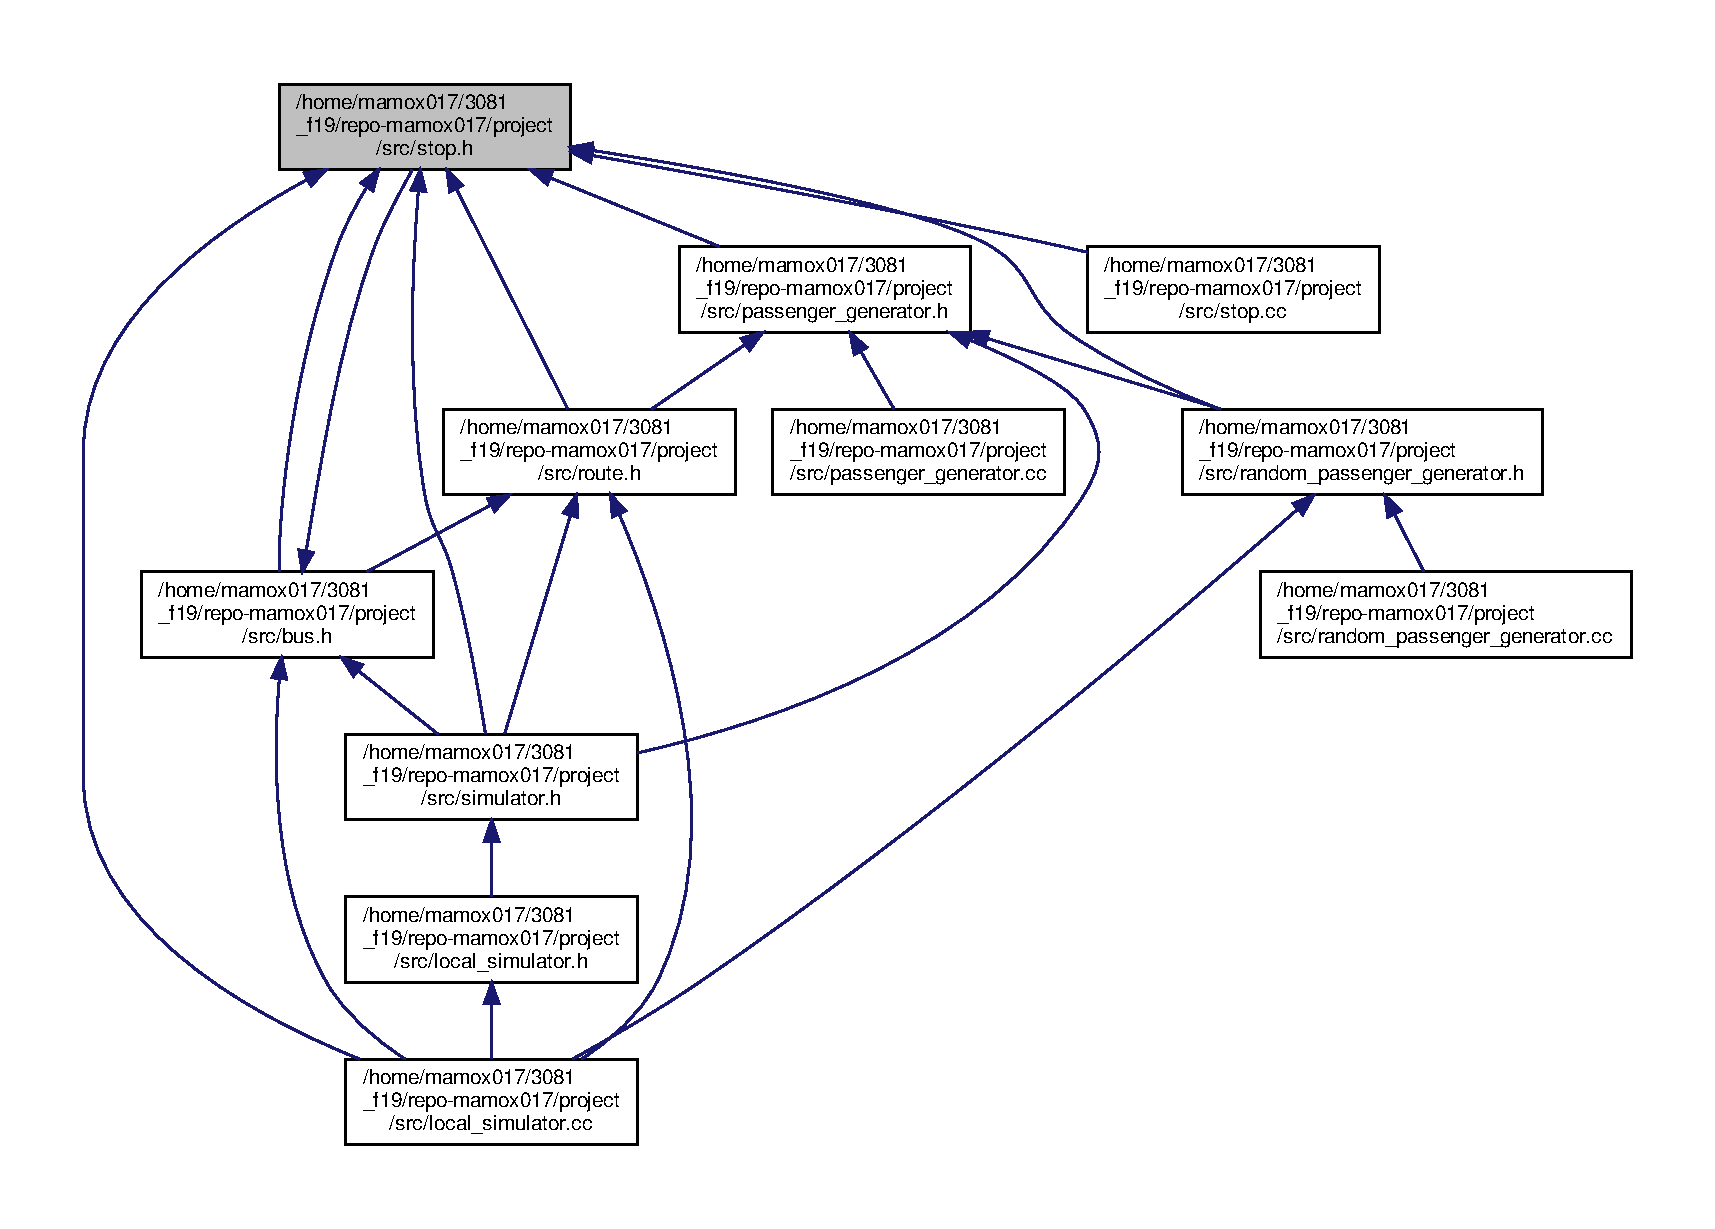
\includegraphics[width=350pt]{stop_8h__dep__incl}
\end{center}
\end{figure}
\subsection*{Classes}
\begin{DoxyCompactItemize}
\item 
class \hyperlink{classStop}{Stop}
\end{DoxyCompactItemize}


\subsection{Detailed Description}
\begin{DoxyCopyright}{Copyright}
2019 3081 Staff, All rights reserved. 
\end{DoxyCopyright}

%--- End generated contents ---

% Index
\backmatter
\newpage
\phantomsection
\clearemptydoublepage
\addcontentsline{toc}{chapter}{Index}
\printindex

\end{document}
